\part{Sexto semestre}
\chapterimage{7.pdf}
\chapter{Geohidrología}
\section{Introducción y generalidades}
\subsection{Objetivos}
\begin{itemize}
    \item Conocer las bases de la geohidrología con el fin de localizar las fuentes de agua subterránea (acuífero) y comprender el funcionamiento de los acuíferos
    \item Aplicar los métodos de cuantificación de la recarga (anual renovable) y la reserva almacenada (no renovable) de los acuíferos para determinar la disponibilidad de agua subterránea para poder llevar a cabo, la explotación del recurso en el contexto de sustentabilidad
\end{itemize}
\subsection{Generalidades}
\begin{definition}[Geohidrología]
    Es el estudio de las aguas subterráneas, el agua subterránea son las que han atravesado el límite de la capa terrestre.
    El riego y drenaje estudian los escasos metros del suelo, cuando en la geohidrología estudia el agua infiltrada en algún lugar donde satura del medio poroso mucho más abajo en los acuíferos.
\end{definition}
\begin{definition}[Acuífero]
    Del latín Aqua (agua) y ferre (llevar). Es un almacenamiento natural de aguas subterráneas. Es una formación geológica capaz de almacenar o permitir el almacenamiento y la movilidad del agua en ellos.
\end{definition}
\begin{definition}[Acuifero sobreexplotado]
    Se usa una cantidad mayor a la que se renova anualmente
\end{definition}
\begin{definition}[Hidrogeología]
    Es el estudio de las aguas subterráneas en el marco geológico
\end{definition}
\subsubsection{Importancia del estudio del agua subterránea}
En la mayor parte del país en donde el clima es desértico o semidesértico, es de considerable importancia la fuente de aguas subterráneas y en muchos casos las aguas subterráneas constituyen la única fuente de abastecimiento de agua para los diferentes usos.
En México el clima desértico está entre los 500 a 800 mm de precipitación pluvial, aquí es donde radica la mayor importancia de las aguas subterráneas, concentradas en el norte del país.

Los recursos hídricos subterráneos son de importancia fundamental por ser la fuente de CONAGUA en 2018:
\begin{itemize}
    \item Suministro de agua potable para uso doméstico (58.4\% del volumen total)
    \item Usos industriales en las ciudades mayores y medianas (52.3\% del volumen total)
    \item Agua de riego para 36.4\% de los 6.5 millones de hectáreas regadas en el país.
\end{itemize}
\subsubsection{Problemática de las aguas subterráneas}
La \textbf{Sobreexplotación} de los acuíferos es uno de los problemas más fuertes de las aguas subterráneas del país, y se define como la condición sostenida de mayor extracción que la recarga del acuífero:
\begin{align*}
    &\text{Entradas}&&>&&\text{Salidas}&&\Longrightarrow&&\text{Acuífero subexplotado}\\
    &\text{Entradas}&&=&&\text{Salidas}&&\Longrightarrow&&\text{Acuífero en equilibrio}\\
    &\text{Entradas}&&<&&\text{Salidas}&&\Longrightarrow&&\text{Acuífero sobreexploado}
\end{align*}
\subsubsection{Características a la sobreexplotación de los acuíferos}
\begin{enumerate}
    \item Abatimiento de los niveles estáticos
    \item Hundimientos y agrietamientos del terreno, afectando infraestructura civil
    \item Disminución del rendimiento de los pozos y de la reserva almacenada
    \item Intrusión salina en acuíferos costeros
    \item Contaminación de las aguas subterráneas por intrusión salina y bombeo de aguas fósiles
    \item Disminución de flujo base en ríos
    \item Agotamiento de manantiales
    \item Desaparición de lagos, humedales y ecosistemas.
\end{enumerate}
En México existen 653 acuíferos para la administración de aguas subterráneas, que aportan el 39\% del volumen para usos consuntivos. De esos 105 están en condición de sobreexplotación, 32 con presencia de suelos salinos y agua salobre, 18 con intrusión marina; en las aguas superficiales se tienen 757 cuencas para la administración de aguas superficiales, 8 cuencas transfronterizas y 51 ríos principales.
\begin{figure}[h!]
\centering
  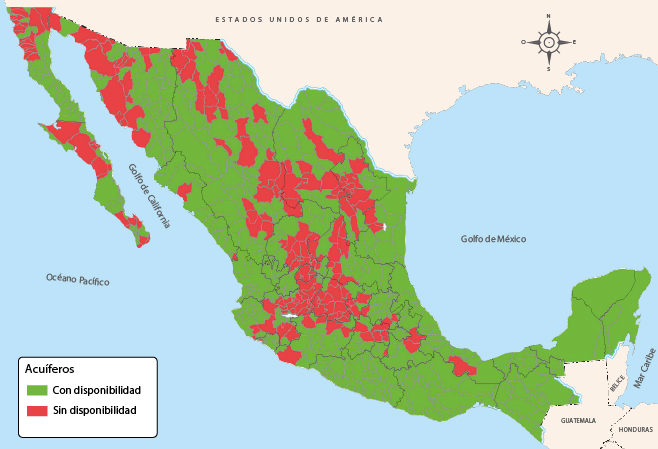
\includegraphics[width=0.5\textwidth]{gh1.jpg}
  \caption{Acuíferos sobreexplotados}
  \label{gh1}
\end{figure}
El abatimiento de los niveles del agua, provoca en forma general, incremento de los costos de bombeo y en forma específica:
\begin{enumerate}
    \item Incremento de los costos de operación por concepto de energía eléctrica o combustibles, al bombear el agua con mayores cargas hidráulicas
    \item Incremento de los costos de inversión, al requerir mayor potencia de motor, pozos más profundos, columnas y flechas de mayor longitud, instalaciones eléctricas de mayor capacidad
    \item Incremento en los costos de mantenimiento; al ser los equipos de bombeo más robustos y los pozos más profundos, los costos de mantenimientos también se ven incrementados. 
\end{enumerate}
El daño a la infraestructura, el algo difícil de calcular en los costos de mantenimiento.

Los hundimientos y agrietamientos, causan inestabilidad, deformaciones y fallas de los diferentes tipos de infraestructura ubicada en la superficie del terreno. La disminución de la reserva almacenada limita y pone en riesgo el desarrollo económico.

Otro problema que presenta las aguas subterráneas es la contaminación. De hecho se consideran a las aguas subterráneas menos vulnerables a la contaminación, sin embargo esto no significa que la calidad de estas esté salvaguardada de todo deterioro; cada vez son más los casos de contaminación de acuíferos. En algunos casos la contaminación es un efecto colateral de la sobreexplotación, como ocurre en los acuíferos costeros. En muchos otros tiene otro origen, como la infiltración excedente de riego en las zonas agrícolas y el desecho de las aguas residuales en zonas urbanas e industriales.

La escasez del recurso en relación con su creciente demanda, ha originado una fuerte competencia entre los diferentes sectores por su aprovechamiento. Las ciudades están acaparando las fuentes de agua para su abastecimiento, con frecuencia a costo de la agricultura. Los complejos industriales en los grandes asentamientos humanos, están complicando el abastecimiento de agua de las poblaciones.
\subsection{Historia de la Geohidrología}
El aprovechamiento del agua subterránea data de varios miles de años. En irán hace más de 2500 años se construyeron grandes galerías de km de longitud llamadas Qanats (muchos continúan en uso)

El agua subterránea fue utilizada por el hombre antes de entender su origen, existencia y movimiento dentro del suelo. Los filósofos griegos y romanos dejaron escritas explicaciones del origen de las fuentes y del agua subterránea, encontrando teorías fantásticas a conocimientos correctos

Hasta antes del siglo XVII se pensaba que el agua que emergía de las fuente brotante se corría de la lluvia era muy poca y que la tierra era demasiado impermeable para permitir la penetración del agua bastante profunda bajo la superficie.

Algunos filósofos como Homero, Tales de Mileto (428-347 a.C) y Platón presentaron una hipótesis acerca de la formación de las fuentes: ``Debido a la conducción del agua del mar a través de conductos subterráneos bajo las montañas, el agua se purificaba y se elevaba a la superficie''

Aristoteles (384-322 a.C) Pensó que el agua subterránea circulaba dentro de un complicado sistema de aberturas y cavernas que jugarían el papel de una gran esponja, siendo el vapor de agua que emanaría desde el interior de la tierra el que aportaría la mayor parte del agua de los manantiales.

Los filósofos romanos como Lucio Anneo Séneca (4-65 d.C) y Plinio (23-79 d.C) siguieron las ideas griegas, negando el fenómeno de la infiltración del agua en el suelo.

El ingeniero y arquitecto romano Marco Vitruvius (15 a.C) explicó la teoría actualmente aceptada de la infiltración de grandes cantidades de agua de lluvia que se reciben en una cuenca, las cuales se percolan a través del suelo o de estratos rocosos y que emergen en las laderas o base de las montañas en forma de fuentes, y sin embargo las otras teorías griegas persistieron por caso 1500 a través de la edad media hasta el renacimiento.

Desde los inicios del pensamiento científico y hasta el renacimiento (hacia el 1600) se hicieron pocos progresos en el campo de la geohidrología. Existieron cinco errores fundamentales en el pensamiento de la mayoría de los grandes filósofos y científico de la antigüedad; estos errores son:
\begin{enumerate}
    \item La tierra no contiene una red de grandes cavernas interiores
    \item El agua del mar no puede perder toda su salinidad por simple filtración a través del subsuelo
    \item El agua de lluvia se infiltra en grandes cantidades.
\end{enumerate}

Leonardo da Vinci (1452-1519) enfocó la teoría de la infiltración en forma notable, teniendo un claro concepto del ciclo hidrológico incluyendo la infiltración del agua y su afloramiento en manantiales.

Los alemanes Johannes Kepler (1571-1630) y el matemático Athanasius Kircher (1602-1680), elaboraron ampliamente las ideas primitivas de Aristóteles y Séneca. Kepler imaginó que la tierra era semejante a un enorme animal que digería el agua del mar y sería el producto final del metabolismo de la tierra.

Finalmente como producto de observaciones y estudios realizados en Francia por Pierre Perrault (1628-1703) y Edmé Mariotte (1620-1684), se demuestra la existencia del ciclo hidrológico y con ello se establecen las bases de la Geohidrología, el agua subterránea es originada por la infiltración del agua de lluvia.

En la primera mitad del siglo XVII fueron perforados muchos pozos artesianos (Artois) en Francia, estimulado así el interés en el agua subterránea.

% POZO ARTESIANO O BROTANTE, ES AQUÉL DONDE EL AGUA SALE SÓLA

Aunque los pozos surgentes (artesianos) despertaron la curiosidad ya desde los tiempos de los griegos, se consiguió dar una explicación correcta del fenómeno. La primera explicación mecánicamente correcta fue dada por el filósofo y científica iraní Sheikh Abu Raihan al-Biruni (973-1048). No obstante, la primera explicación verdaderamente documentada fue aportada por Antonio Vallisnieri, rector de la Universidad ed Padua (Italia), quien en 1915 publicó un artículo sobre los pozos surgentes del norte de Italia.

El ingeniero hidráulico francés Henry Darcy estudió el movimiento del agua a través de las arenas. En un apéndice del informe sobre el proyecto de abastecimiento de agua potable de Dijon publicado en 1856, definió la relación conocida ahora como la Ley de Darcy; la cual gobierna el movimiento del agua en la mayoría de las formaciones aluviales sedimentarias
\begin{equation}
    v =-ki =-k\frac{\Delta h}{L}
\end{equation}
% flujo potencial: Flujo de calor y flujo de agua

Jules Dupuit desarrolló en 1863 una fórmula para el estudio del flujo del agua hacia el interior de un pozo, aplicando la Ley de Darcy

En 1870 el alemán Adolph Thiem modificó la fórmula de Dupuit con objetivo de hacerla aplicable en la obtención de las características hidráulicas de un acuífero mediante el bombeo de un pozo y la observación de los efectos producidos en pozos vecinos.

El primer modelo de flujo es atribuido a Philip Forchheimer, cuando construyó un modelo físico de arena para estudiar el flujo de agua hacia un pozo en Graz Austria en 1898.

En 1935 se inicia una etapa floreciente con una de las aportaciones más trascendentes: el desarrollo de una ecuación para describir el flujo del agua hacia un pozo en régimen transitorio (primeramente po C.V. Theis y después por C.E. Jacob). Desde este año se acelera el progreso de la Geohidrología destacando los logros en los suficientes campos: como hidráulica de pozos, la evaluación geohidrológica, la simulación del comportamiento de acuíferos, etc.
\begin{equation}
    a=\frac{Q}{4\pi T}\int_{u}^{\infty} \frac{e^{- u}}{u}\, dv
\end{equation}

Los primeros modelos de simulación de acuíferos, aparecieron en el primer cuarto del siglo pasado y eran principalmente de arena; y a partir de 1960 es cuando empieza un vertiginoso desarrollo, basado fundamentalmente en modelos analógicos eléctricos y uso de computadoras

A mediados de la década de los 60s, los modelos de analogía eléctrica fueron desplazados por los métodos numéricos basados en diferencias finitas (bidimensionales), por el corto tiempo entre la concepción del modelo y la realización de éste, además de la disponibilidad del equipo requerido para el mismo.

En la década de los 90's se desarrollaron modelos de simulación de flujo de masa y de solutos tridimensionales en diferencias finitas y elementos finitos.

Balance anual en $Km^3$ (CONAGUA, 2009), en poco menos de $2\times 10^{6}$ de $km^2$, con una precipitación media anual de 740mm, la conversión es $1km^3=1000\times 10^6m^3$
\begin{figure}[h!]
\centering
  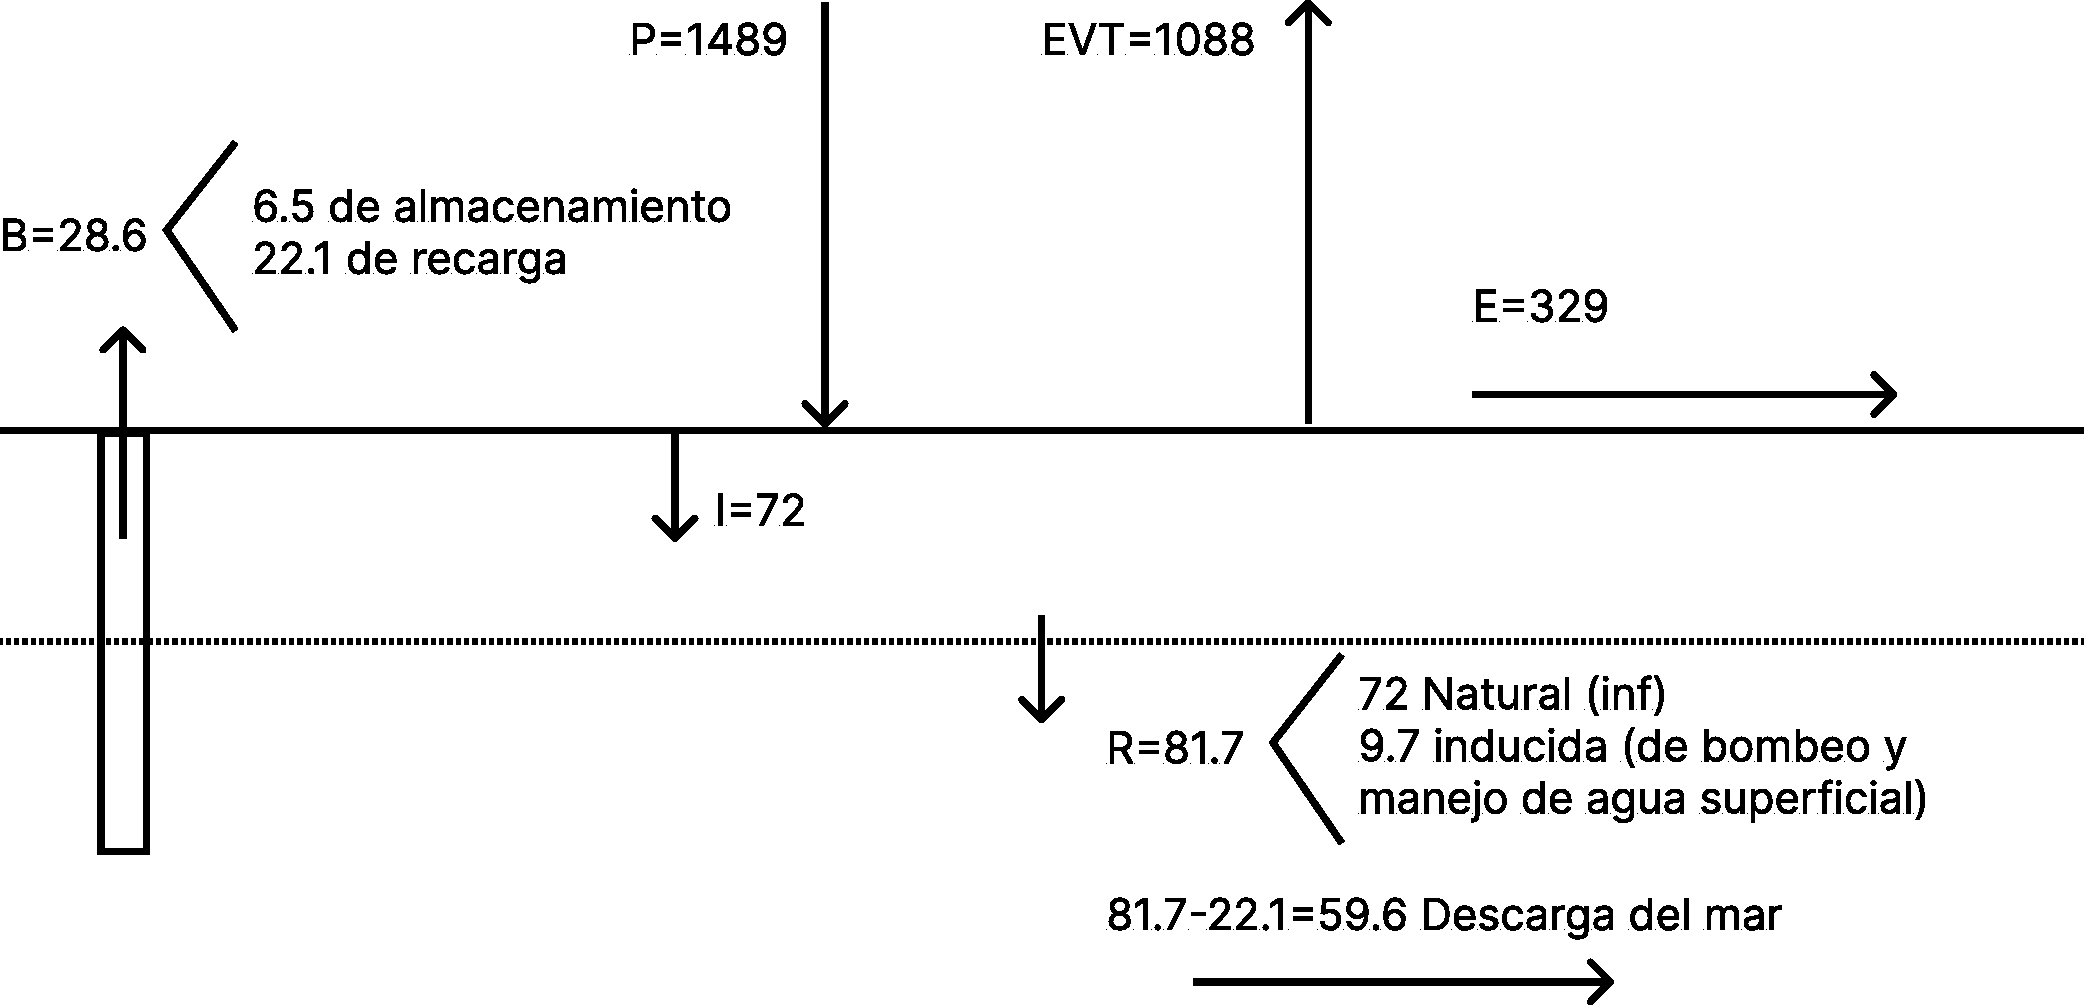
\includegraphics[width=0.8\textwidth]{gh2.pdf}
  \caption{Balance Hídrico Nacional}
  \label{gh2}
\end{figure}
\subsubsection{Estudio del agua subterránea}
Etapas:
\begin{enumerate}
    \item Prospección: Métodos directos (mediante perforaciones exploratorias) e indirectos
    \item Cuantificación: Balance, cuánta agua hay en el acuífero y cuánta recarga
    \item Predicción: Modelos de simulación de acuíferos para estudiar escenarios a tendencias de cinco a diez años
    \item Optimización: Cómo distribuir volúmenes de agua temporal y espacialmente y a qué actividad económica lo dedican
\end{enumerate}
La mayoría sólo llegan a la etapa de cuantificación.
\begin{figure}[h!]
    \centering
      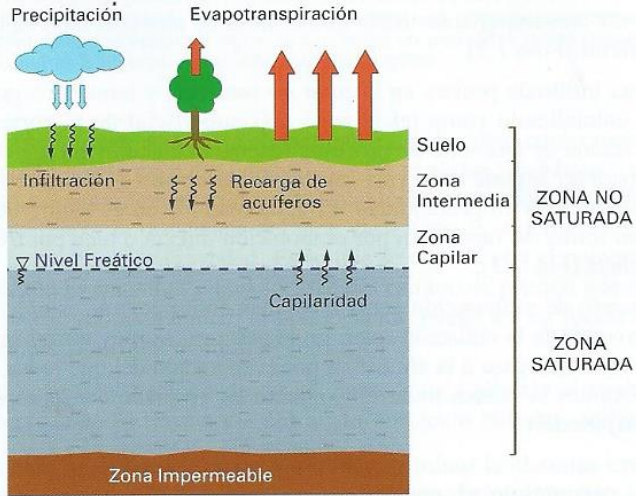
\includegraphics[width=0.5\textwidth]{gh3.png}
      \caption{Clasificación de zonas del subsuelo por comportamiento del agua que se infiltra (MartínezAlfaro et al., 2005)}
      \label{gh3}
    \end{figure}
    Nótese que en la figura \ref{gh3}, los diámetros de las partículas es menor la capilaridad, el agua llega hasta una zona impermeable de rocas ígneas, metamórficas o sedimentarias que ya no permite la infiltración del agua,
    a ésta zona hasta el nivel freático se le conoce como zona saturada. La zona intermedia es definida a partir del término de los horizontes del suelo y la zona capilar.
\section{Conceptos básicos}
\begin{definition}[Porosidad]
    Proporción de vacíos del volumen total de un suelo o roca.
    \begin{equation}
        n = \frac{v_t - v_s}{v_t} = \frac{v_v}{v_t}
    \end{equation}
    Entre los suelos más porosos, encontramos aquellos, producto de la acumulación del resquebrajamiento de partículas, a causa de aberturas de raíces y madrigueras de animales.
\end{definition}
La porosidad de depósitos no consolidados está en función del arreglo, forma y tamaño de partículas de roca.
\begin{table}[h!]
    \centering
    \begin{tabular}{@{}cc@{}}
    \toprule
    Material      & Porosidad (\%) \\ \midrule
    Arcilla       & 44-55          \\
    Arena         & 35-40          \\
    Grava         & 30-40          \\
    Grava y arena & 20-35          \\
    Arenisca      & 10-20          \\
    Caliza        & 1-10           \\
    Basalto        & 1-10           \\ \bottomrule
    \end{tabular}
    \caption{Valores de porosidad para algunos materiales}
    \label{tabgh1}
\end{table}
\begin{figure}[h!]
\centering
  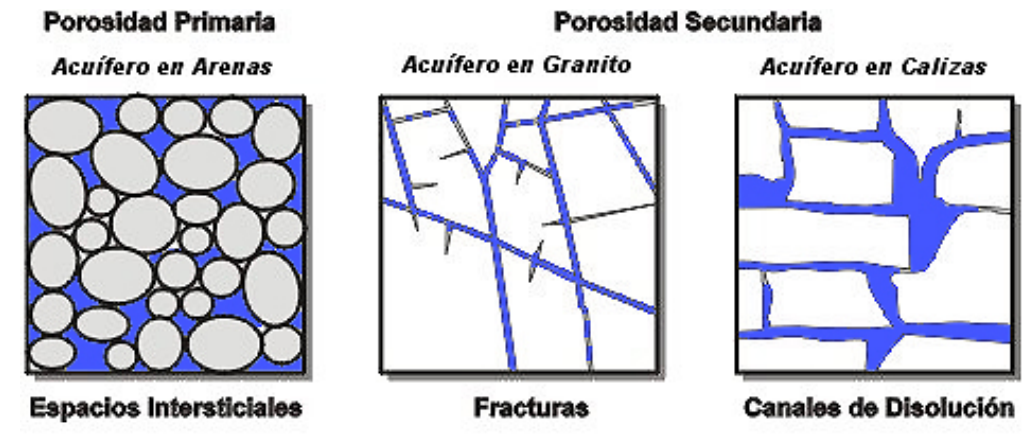
\includegraphics[width=0.8\textwidth]{gh4.png}
  \caption{Almacenamiento: A menor escala, a más pequeño el grano mayor es la porosidad }
  \label{gh4}
\end{figure}
\subsection{Rendimiento específico y retención específica}
La porosidad es importante en el estudio del agua subterránea.
El \textbf{rendimiento específico} expresa cuánta agua es aprovechable para uso del hombre, y la \textbf{retención específica} expresa cuánta agua permanece en la roca después de que es liberada por gravedad.
\begin{align}
    &S_y = \frac{V_d}{V_t}\\
    &S_r = \frac{V_r}{V_t}
\end{align}
Esto se puede explicar gráficamente:
\begin{enumerate}
    \item Si se tiene $1m^3$ de material poroso completamente seco, y adicionalmente agua suficiente para saturarlo, es decir para que todos sus poros estén totalmente llenos de agua.
    \item El volumen de agua que se requiere para saturar ese $1m^3$ de medio poros es precisamente igual a su porosidad
    \item Éste sería el medio poroso completamente saturado (acuífero), ahora si de este, se permite que el agua se drene solamente por acción de la gravedad
    \item Se liberará un volumen de agua que será igual al rendimiento específico ($S_y$)
    \item Un cierto volumen es retenido por las partículas sólidas del medio poroso, en contra de la acción de la gravedad este volumen será igual a la retención específica $S_r$
\end{enumerate}
Como el volumen drenado más el volumen retenido es igual al volumen de vacíos entonces:
\begin{equation}
    n = S_y+ S_r
\end{equation}
\begin{table}[h!]
    \centering
    \begin{tabular}{@{}ccc@{}}
    \toprule
    Material      & $S_y$ (\%) & $S_r$ (\%) \\ \midrule
    Arcilla       & 1-10       & 40-50      \\
    Arena         & 10-30      & 10-25      \\
    Grava         & 15-30      & 10-15      \\
    Grava y arena & 15-25      & 5-10       \\
    Arenisca      & 5-15       & 5          \\
    Caliza        & 0.09       & 0.01       \\
    Basalto        & 8          & 2          \\ \bottomrule
    \end{tabular}
    \caption{Valores de retención específica y rendimiento específico de algunos materiales}
    \label{tabgh2}
\end{table}
\subsection{Contenido de humedad, deficiencia de humedad y grado de saturación}
El contenido de humedad de una roca es la cantidad de agua que se encuentre en sus poros por unidad de volumen roca, esto es:
\begin{equation}
    \theta = \frac{v_w}{v_t}
\end{equation}
Cuando la roca está totalmente saturada, el contenido de humedad es numéricamente igual a la porosidad, ¿Existe un $\theta= 100\%$? La respuesta es no, pues teóricamente sería todo un poro, o un 100\% de agua con respecto al suelo.

La deficiencia de humedad, se define como la diferencia entre la retención específica y el contenido de humedad, cuando $\theta< Sr$; por el contrario, si el contenido de humedad es igual o mayor que la retención específica, la deficiencia de humedad es igual a cero.
\begin{align}
    &D_h = S_r -\theta\implies\theta <S_r\\
    &D_h = 0 \implies\theta \geq S_r
\end{align}
En otras palabras, la deficiencia de humedad es la cantidad de agua que requiere una roca por unidad de volumen para satisfacer su retención específica.

El grado de saturación es la relación entre la cantidad de agua que contiene un material y su volumen de vacíos, se expresa como un porcentaje (0 a 100)
\begin{equation}
    G_s = \frac{V_w}{V_v}
\end{equation}
\begin{problem}
El bloque de material poros es una combinación de grava y arena, de la figura está a un contenido de humedad ($\theta$) de 5\%, su retención específica es de 8\% y su rendimiento específico es 23\%. Bajo la hipótesis: Base impermeable, $Evt=0$ y movimiento vertical tipo pistón (Green y Ampt, 1911).
\begin{enumerate}
    \item El volumen necesario de aua para que el grado de saturación del bloque sea de 100\%
    \item El volumen de agua para satisfacer el déficit de humedad del boque
    \item El volumen de agua aprovechable si el material está completamente saturado
    \item El contenido de humedad que tendrá el bloque si recibe una precipitación de 620mm
    \item El contenido de humedad que tendrá el bloque si la precipitación es 3,520mm 
\end{enumerate}
\end{problem}
\begin{figure}[h!]
\centering
  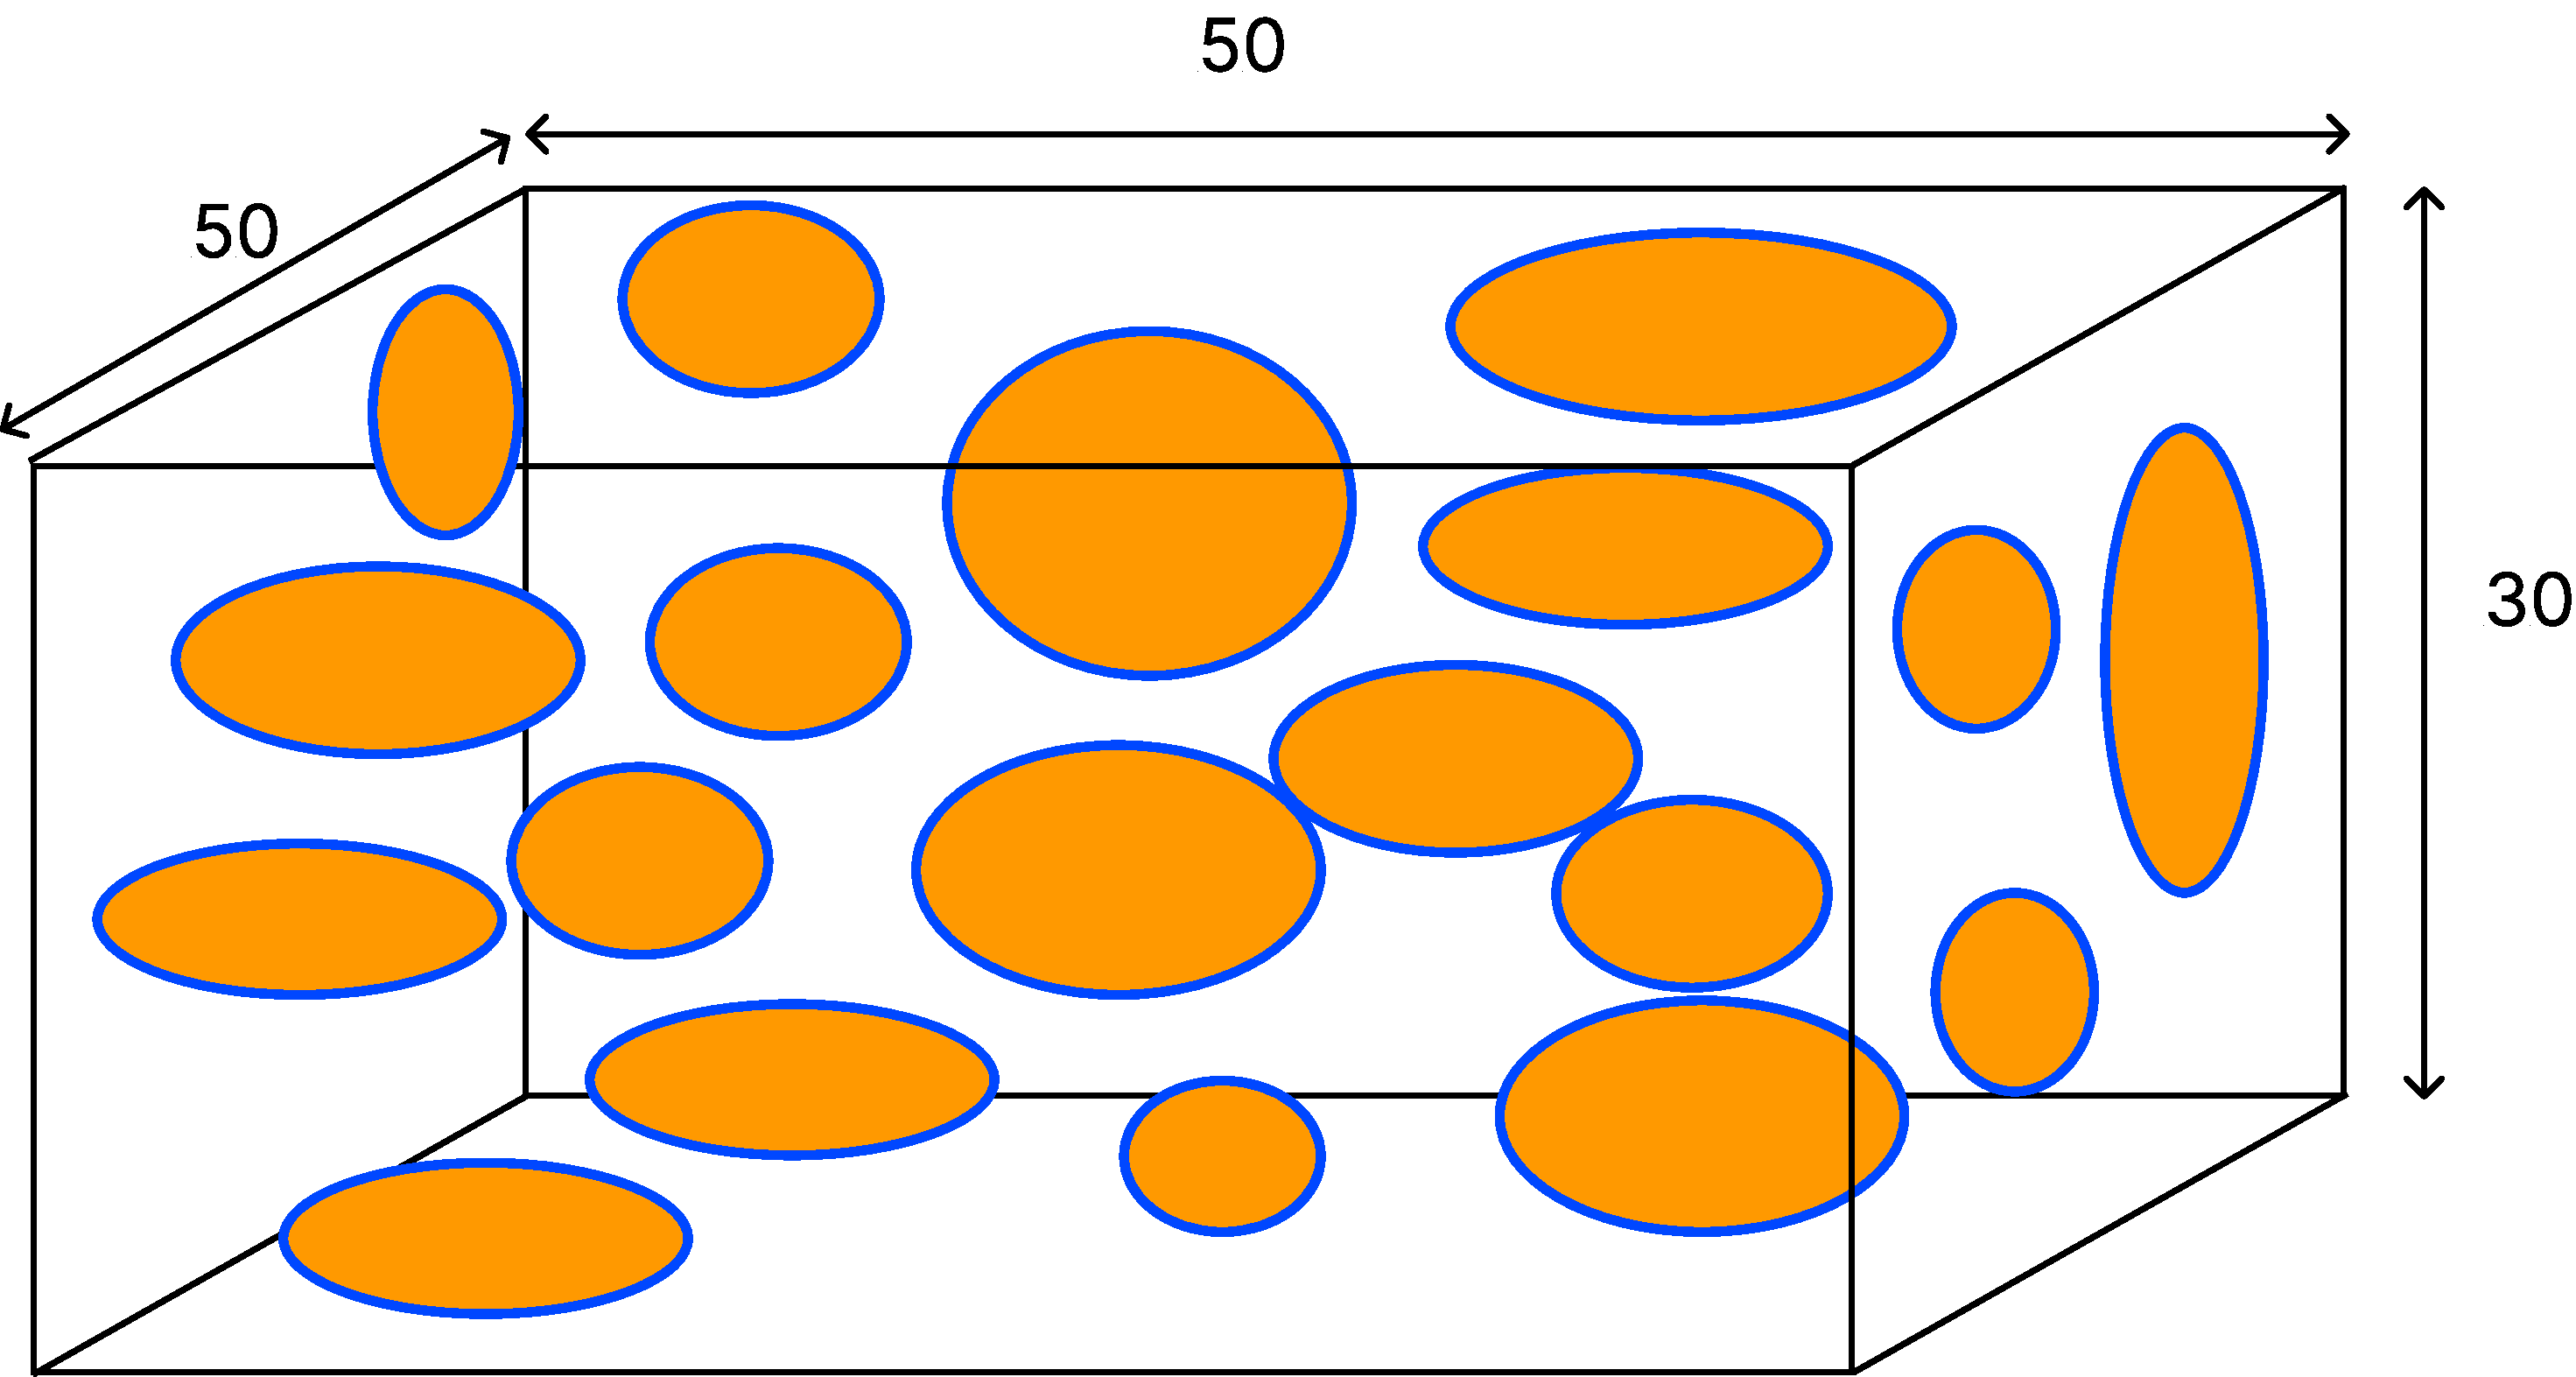
\includegraphics[width=0.5\textwidth]{gh5.pdf}
  \caption{Esquema del problema}
  \label{gh}
\end{figure}
\textit{ Sol. }

El volumen de agua para que el bloque pase de $\theta_i=5\%$ a $G_g=100\%$, en términos de contenido de humedad, $G_s=100\%$ equivale a $\theta_n=31\%$, es decir que todos los poros están totalmente ocupados por agua, así:
\begin{equation*}
    Vol= V_t\left(n -\theta_i\right) =50m\cdot50m\cdot 30m\left(0.31 - 0.05\right) =19500m^3
\end{equation*}
Esto equivale a una lámina de agua sobre la superficie del bloque de
\begin{equation*}
    L = \frac{Vol}{A} = \frac{19500}{50 \cdot 50} = 7.8 = 7800mm
\end{equation*}
El volumen de agua para satisfacer el déficit de humedad del bloque:
\begin{equation*}
    Vol = V_t \cdot D_h = V_t\left(S_r -\theta_i\right)= 75000m^3\left(0.08 - 0.05\right)= 2,250m^3
\end{equation*}
Que en términos de lámina será:
\begin{equation*}
    L = \frac{Vol}{A} = \frac{2250}{2500} = 0.9m
\end{equation*}
Volumen de agua aprovechable si el bloque está completamente saturado
\begin{equation*}
    Vol = V_t \cdot S_y =75000(0.23) =17250m^3
\end{equation*}
% Contenido de humedad del bloque si la precipitación sobre él es de 620mm, esto último equivale a una lámina de 0.62m de agua, lo que en términos de volumen sobre la superficie del bloque serán $Vol=A*L=2500m^2*0.62$ Y este valor es intermedio entre el volumen necesario para satisfacer el déficit de humedad ($2250m^3$) y el volumen para saturar con

% El contenido de humedad del bloque si la precipitación sobre él es de 3520mm. En éste caso, el volumen precipitado será de $2500m^2*3.52=8800m^3$.

% \begin{align*}
%     &V_{precip} = A\cdot p\\
%     &V_{precip} = (2500m^3)(3.52m) = 8800m^3\\
%     &\implies 8800 - 2250m^3 = 6550m^3
% \end{align*}
% Como $\theta_0=5\%$, $\theta_{sr}=8\%$ y $S_y=23\%=17250\implies 30m$, el rendimiento es 6550, el $Dh=2250$
\subsection{Carga y gradiente hidráulico}
% La profundidad

Si en un punto de un acuífero se introduce la boca de un tubo desde la superficie, la presión del agua en ese punto hará que el agua ascienda dentro del tubo hasta una altura tal, que el peso de la columna de agua por unidad de área, equilibre la presión en el punto considerado. La altura del nivel del agua sobre éste es igual a la carga de presión, así:
\begin{equation}
    H = Z + H_p
\end{equation}
El gradiente hidráulico es el cambio en carga por unidad de distancia en una dirección dada, para calcularse se emplea la siguiente fórmula
\begin{equation}
    i= \frac{\Delta h}{L}
\end{equation}
\begin{figure}[h!]
\centering
  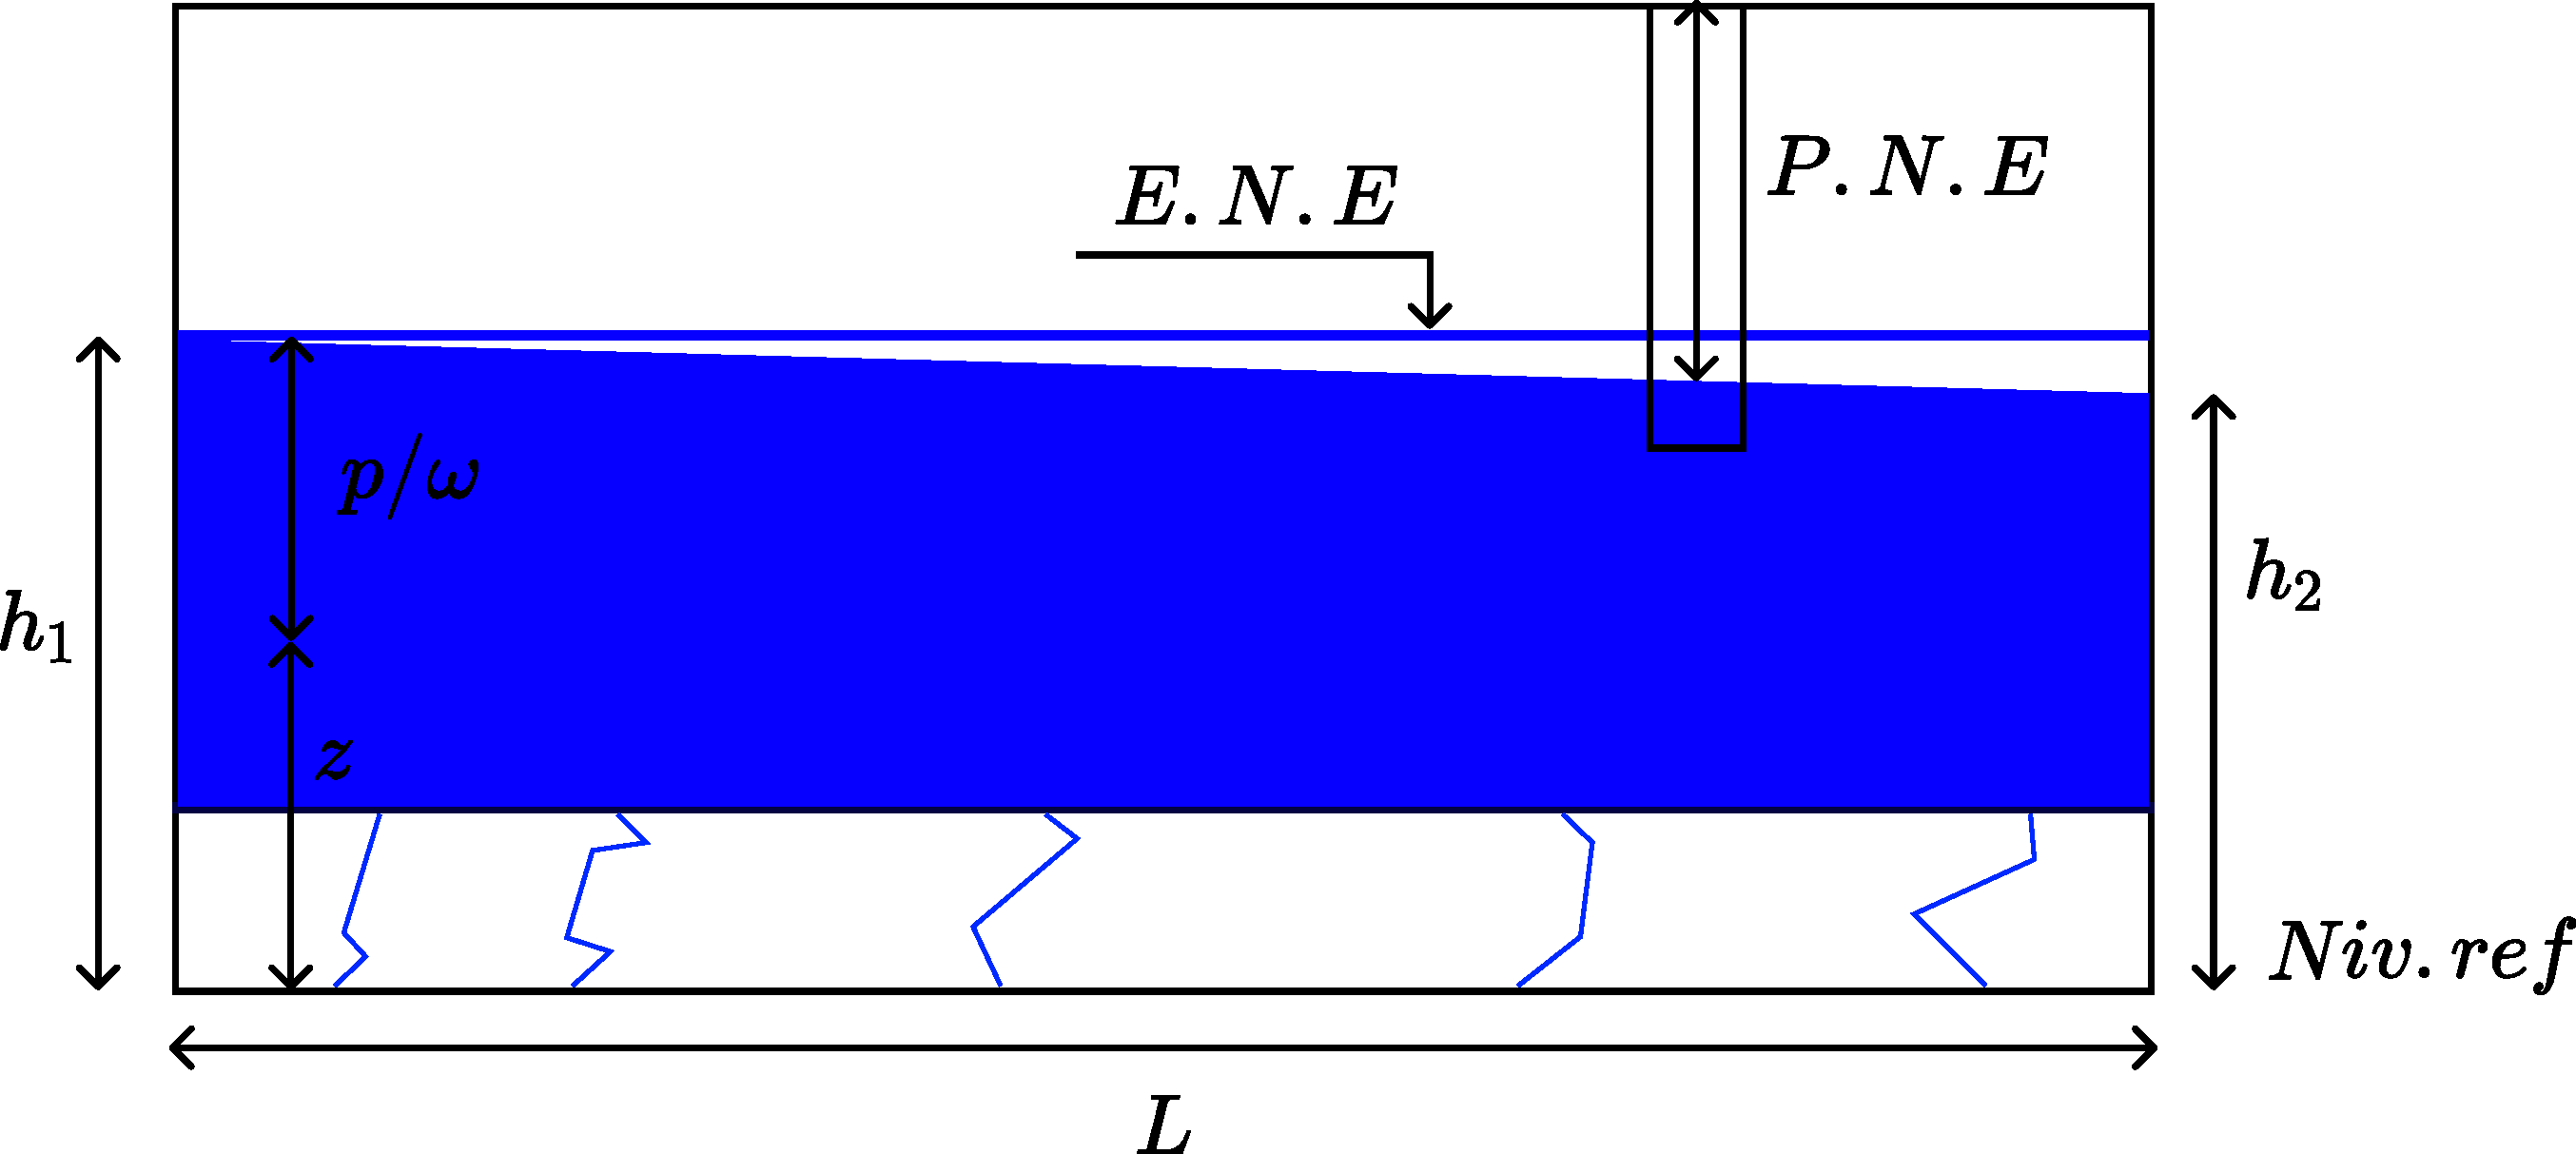
\includegraphics[width=0.5\textwidth]{gh6.pdf}
  \caption{Esquema de un acuífero con la carga y gradiente hidráulico.}
  \label{gh6}
\end{figure}

\subsection{Permeabilidad (K)}
La permeabilidad es la propiedad del material acuífero que consiste en transmitir el agua bajo presión y/o capacidad de una roca para permitir la circulación del agua a través de ella. Cuantitativamente su valor está dado por el coeficiente de permeabilidad de Darcy. Esta propiedad depende de la forma, acomodo y distribución granulométrica de las partículas constituyentes y del grado de compactación o cementación de las mismas, factores que controlan, a su vez, el tamaño e interconexión de los intersticios. El coeficiente de permeabilidad expresa en unidades de velocidad, generalmente en m/s ó cm/s.

Es importante destacar que permeabilidad puede darse de dos formas: Debido al paso del agua a través de los huecos que dejan entre sí las diversas partículas que forman las rocas (porosidad) y debido a las grietas, roturas, fisuras que aparecen en su interior (fisuramiento).

Una capa arenosa es impermeable por porosidad, mientras que una roca de caliza marmórea no lo es; sin embargo, tal caliza, en su estado natural y en grandes masas, suele resultar permeable por fisuración a causa de las grietas que la atraviesa; por consiguiente una elevada porosidad no implica necesariamente una elevada permeabilidad, por el contrario.
\begin{table}[h!]
    \centering
    \begin{tabular}{@{}cccc@{}}
    \toprule
    Material    & Porosidad (\%) & Ren. Esp. (\%) & Permeabilidad (m/s)                   \\ \midrule
    Arcillas     & 45-55          & 1-10           & $10\times^{-10}$ a $2\times 10^{-7}$  \\
    Arena       & 35-40          & 10-30          & $10\times^{-5}$ a $3\times 10^{-4}$   \\
    Grava       & 30-40          & 15-30          & $10\times^{-4}$ a $1.5\times 10^{-3}$ \\
    Grava-Arena & 20-35          & 15-25          & $10\times^{-5}$ a $5\times 10^{-4}$   \\
    Arenisca    & 10-20          & 5-15           & $10\times^{-8}$ a $5\times 10^{-6}$   \\
    Caliza      & 1-10           & 1-5            & Muy variable                          \\ \bottomrule
    \end{tabular}
    \caption{Porosidad, rendimiento específico y permeabilidad}
    \label{tabgh222}
\end{table}
\subsection{Ley de Darcy}
En 1856 Henry Darcy estudió experimentalmente el fenómeno del flujo de agua a través de filtros de arena. Como resultado de sus observaciones estableció la ley de Darcy, la cuál constituye una de las bases de la teoría del flujo en medio porosos. De acuerdo con esta ley, la velocidad con que circula un fluido a través de un material poroso, es directamente proporcional al gradiente hidráulico (válida para flujo laminar, $Re<1$, $Re=dv/Y$, $d_e=d_{10}$ en una curva granulométrica):
\begin{equation}
    V= ki= k \frac{\Delta h}{L}
\end{equation}
Donde $k$ es el coeficiente de permeabilidad o conductividad hidráulica.

Resulta evidente que si el gradiente hidráulico es adimensional, el coeficiente de permeabilidad tiene unidades de velocidad.

La ley de Darcy, es indispensable en la cuantificación de volúmenes de agua que circulan a través de medios porosos. $Q=AV$,A es el área total:
\begin{equation}
    Q=Ak\cdot \frac{\Delta h}{L}
\end{equation}
\begin{figure}[h!]
\centering
  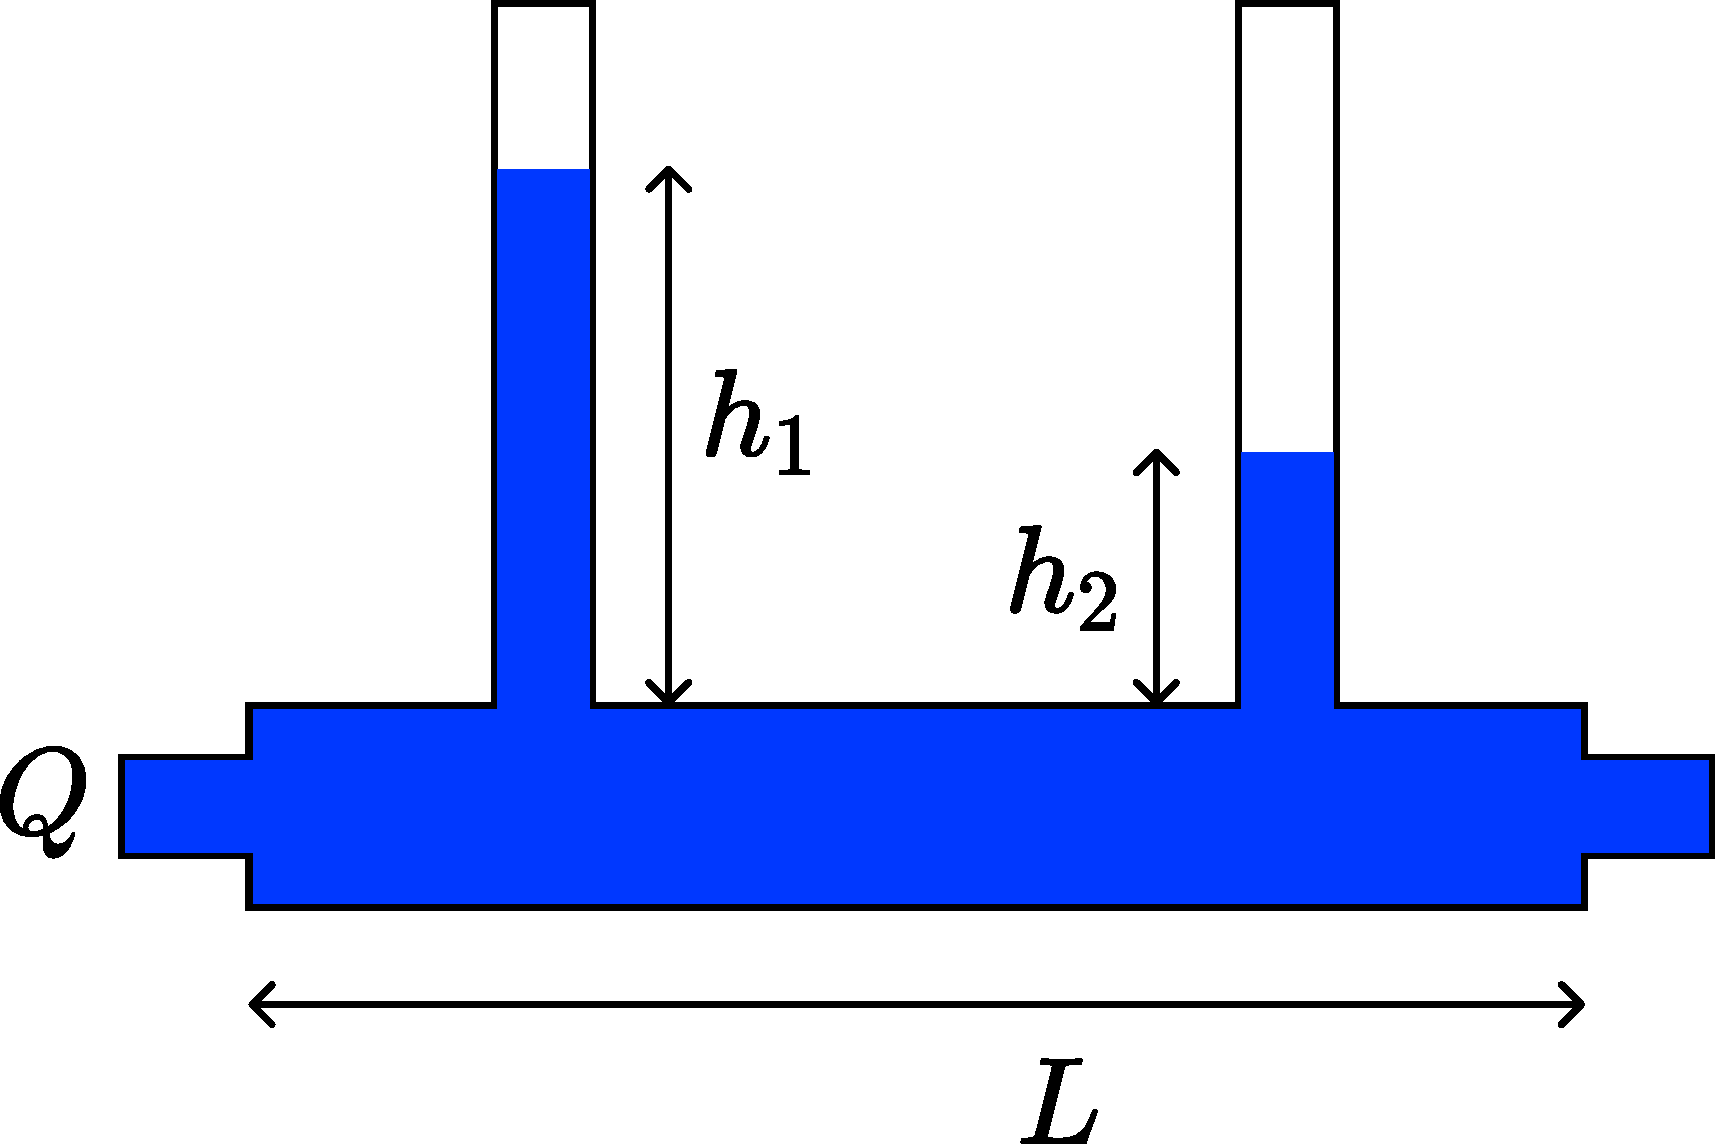
\includegraphics[width=0.5\textwidth]{gh7.pdf}
  \caption{Ley de Darcy}
  \label{gh7}
\end{figure}
La permeabilidad es numéricamente igual al gasto, que fluye en un medio poroso de área transversal al flujo del área unitaria bajo un gradiente hidráulico unitario

La conductividad hidráulica depende de la forma y arreglo de los conductos transmisores (poros y fracturas) además de las características dinámicas del fluido como viscosidad cinemática, densidad y la resistencia del campo gravitacional.

Para considerar por separado la influencia de las características del medio poroso y las

\subsubsection{Velocidad real}
En realidad, como el agua circula únicamente a través del os espacios vacíos, el área de flujo o efectiva es mucho menor que el área trasversal total de la sección, y por lo mismo, la velocidad de circulación es mucho mayor que la velocidad aparente calculada por la Ley de Darcy. El área de flujo o área de filtración ($A_f$), está dada por la fórmula:
\begin{equation}
    A_f= An_e
\end{equation}
Siendo $n_e$, la porosidad efectiva, la cual es menor que la porosidad total debido a que esta última, toma en cuenta la parte de los vacíos que es ocupada por agua pelicular adherida a las paredes de las partículas, por continuidad:
\begin{align}
    &Q = VA =V_rA_f\\
    &v_r=\frac{VA}{A_f}=\frac{ki\cdot A}{A\cdot n_e}=\frac{ki}{n_e}
\end{align}
considerando que la porosidad efectiva es numéricamente igual al rendimiento específico, tenemos que.
\begin{equation}
    V_r =\frac{ki}{S_r}
\end{equation}
Puesto que $S_r$ toma valores entre 0.05 y 0.3, resulta que la velocidad real puede ser de 3 a 20 veces mayor que la velocidad aparente.

El concepto de velocidad real tiene primordial importancia en problema de contaminación, pues representa la rapidez con que se propaga un contaminante en el subsuelo.

\subsection{Transmisividad}
Es la capacidad de un acuífero para transmitir agua. La transmisividad de un acuífero es igual a la conductividad hidráulica del mismo multiplicada por su espesor saturado:
\begin{equation}
    T = kb
\end{equation}

\begin{align*}
    &T = kb =2.3\times 10^{- 4} \frac{m}{s}(100m) = 2.3\times 10^{ - 2}\frac{m^2}{s}\\
    &Q = A\cdot V = A\cdot ki = Bb\cdot ki = Bt\frac{\Delta h}{L} = 1000m\left( 2.3\times10^{ - 2} \frac{m^2}{s}\right)\frac{2.7m}{1000m} = 0.0621\frac{m^3}{s}\\ 
    &Q = \frac{0.0621m^3}{s}\left(\frac{3600s}{h}\right)\left(24\cdot\frac{365h}{\text{año}}\right) = 1 ,958,386\frac{m^3}{t\text{año}}\\
    &V = ki = 0.00000062\frac{m}{s}\quad \frac{V^2}{2g} = 0.0000000000000196m
\end{align*}
Cálculo del número de Reynolds
\begin{equation*}
    Re = \frac{V\cdot De}{\upsilon} =\frac{ki\cdot De}{\upsilon} =\frac{2.3\times 10^{ - 4} \frac{m}{s}\left(\frac{2.7}{1000}\right)0.001m}{1.01\times 10^{ - 6} \frac{m^2}{s}} = 0.0006148 < 1
\end{equation*}
Y por lo tanto el flujo es laminar
\subsection{Tipos de acuíferos}
Son formaciones geohidrológicas que se tienen siempre presiones, aunque se puedan hacer simplificaciones partiendo de ciertas hipótesis como: los acuíferos son en su composición uniformes, horizontales y tubulares.

Los acuíferos pueden dividirse en tres tipos: Acuíferos confinados, libres y semiconfinados. 
El acuífero libre se encuentra en contacto directamente con la atmósfera. Está limitado superiormente por le nivel freático, el cual define directamente su espesor y en su parte inferior por una capa impermeable, Haciendo una analogía con obras hidráulicas, puede decirse que el acuífero libre se comporta como un canal.
\begin{figure}[h!]
\centering
  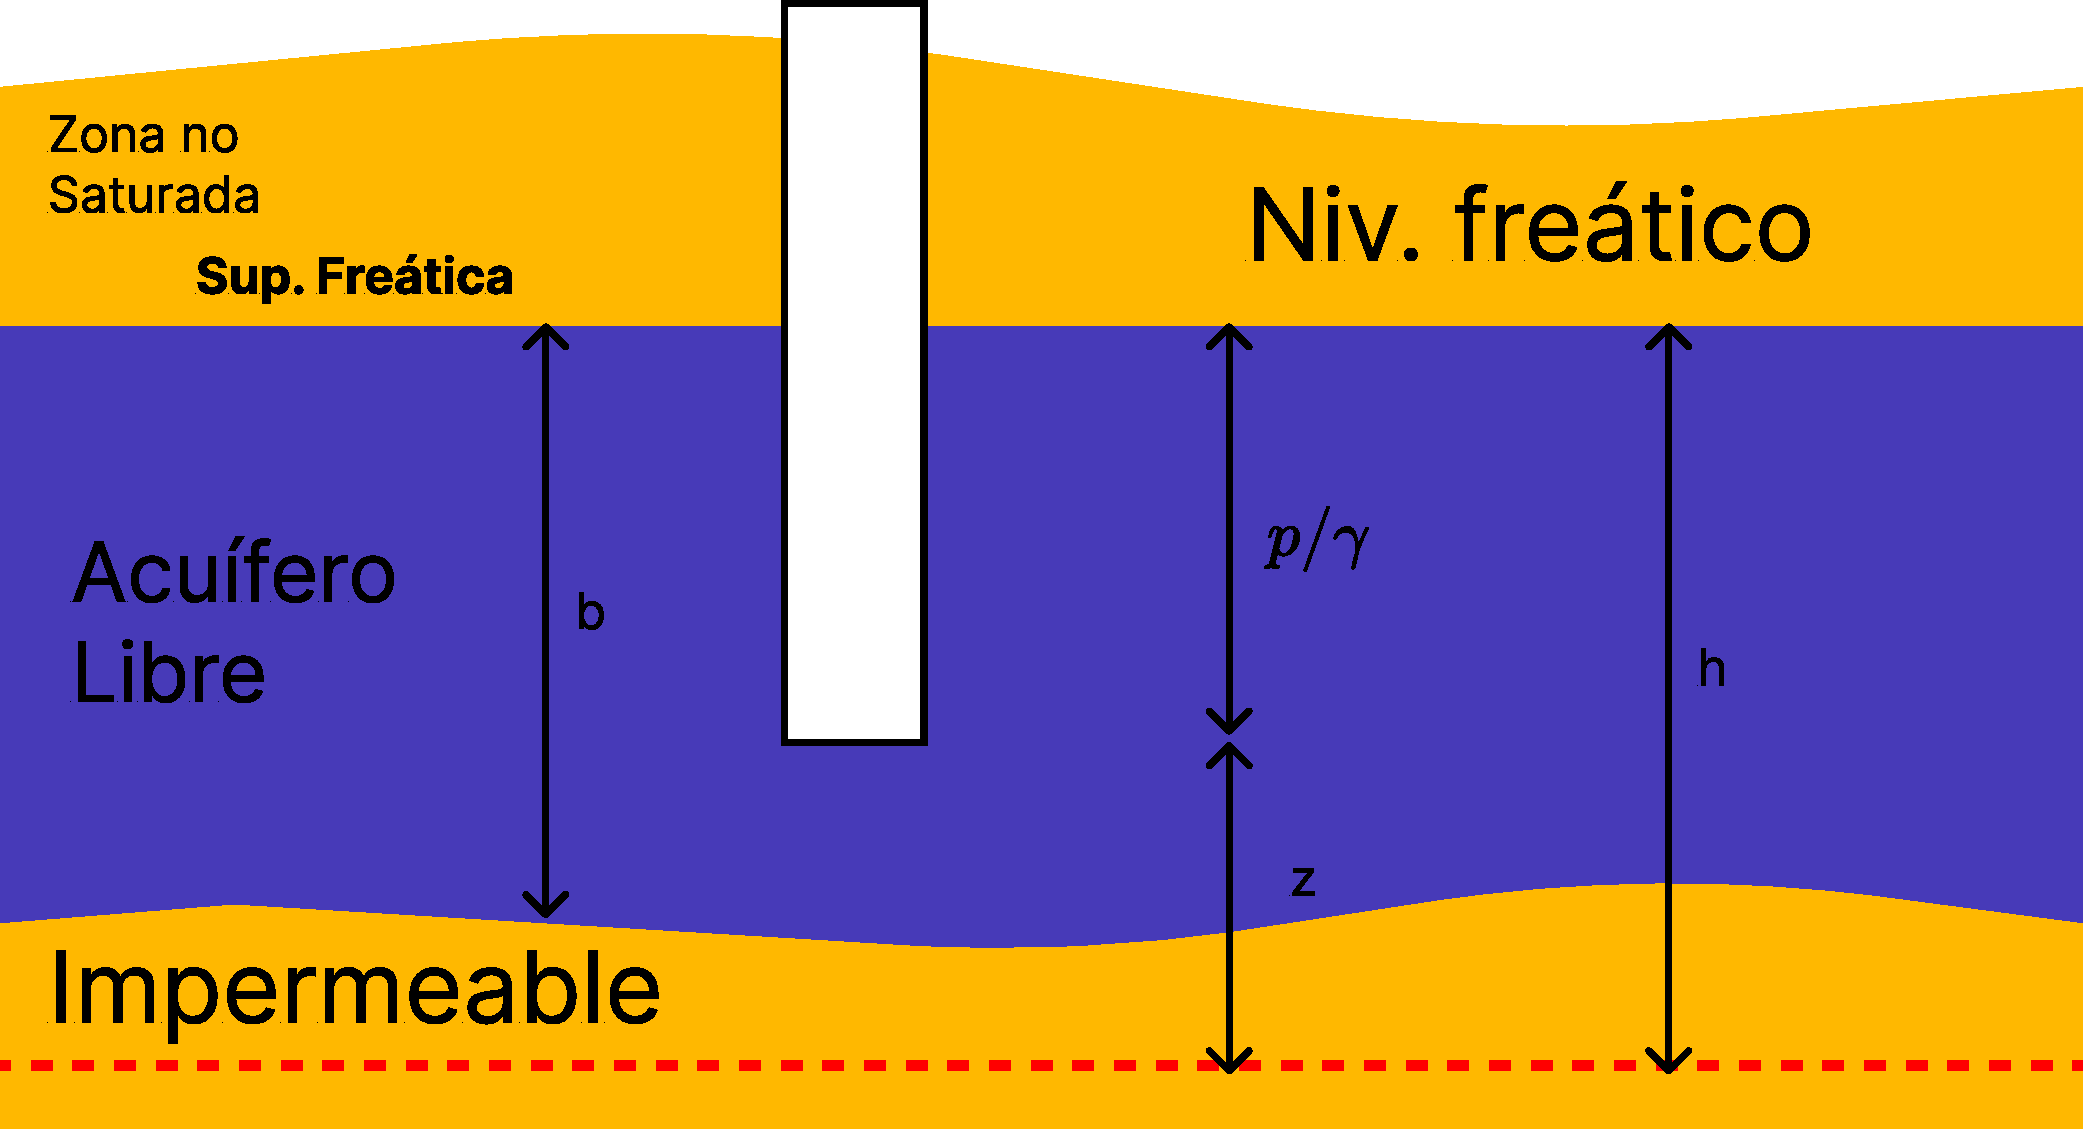
\includegraphics[width=0.5\textwidth]{gh8.pdf}
  \caption{Acuífero libre}
  \label{gh8}
\end{figure}
El acuífero confinado, está separado de la atmósfera por una capa impermeable. Su espesor es la distancia entre las dos capas impermeables que lo limitan. El agua se encuentra a mayor presión que la atmosférica, por lo tanto; al nivel que alcanza el agua en un pozo (artesiano), se le denomina piezométrico. Alguno de estos acuífero poseen carga hidráulica lo suficientemente fuerte para que el agua del pozo sea surgente.
\begin{figure}[h!]
\centering
  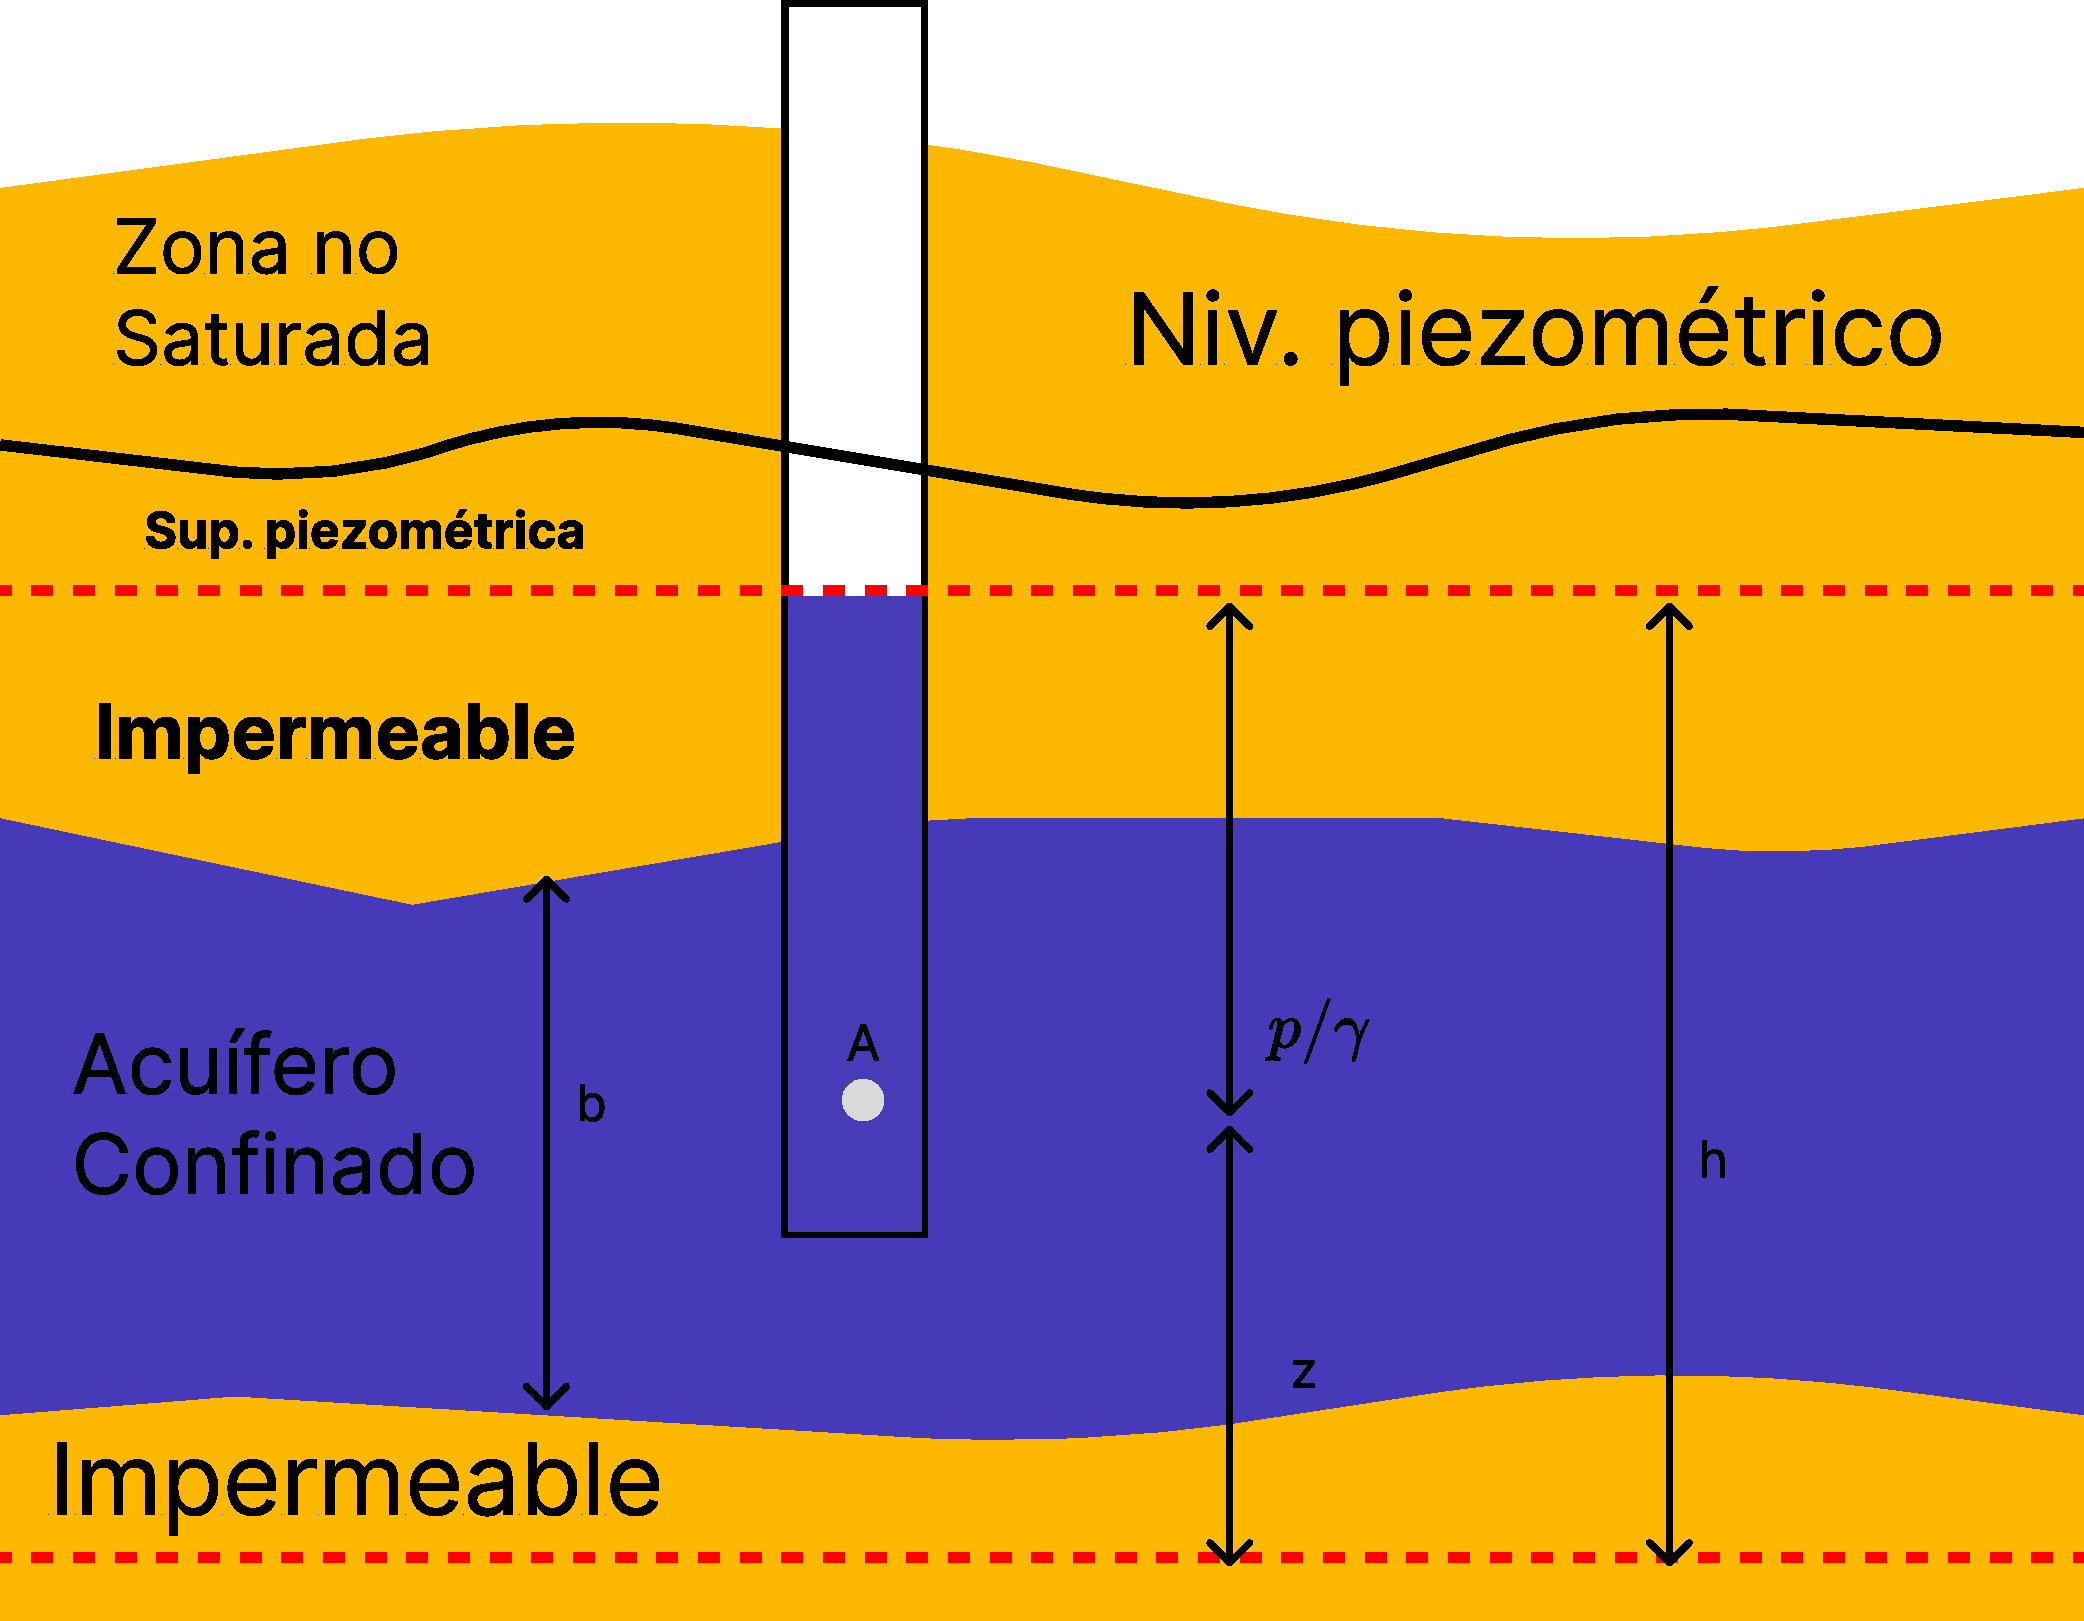
\includegraphics[width=0.5\textwidth]{gh9.pdf}
  \caption{Acuífero confinado}
  \label{gh9}
\end{figure}
Artículo 231 de Ley federal de derechos en materia de agua (2022)

Tratándose de aguas subterráneas, la determinación será por acuífero aplicando la siguiente fórmulas:
\begin{equation}
Idas=\frac{Dma}{(R-Dnc)}
\end{equation}
\begin{notation}
    \begin{itemize}
        \item $Idas=$ Índice de disponibilidad
        \item $Dma=$ Disponibilidad media anual de agua subterránea en una unidad hidrogeológica
        \item $R=$ Recarga total media anual
        \item $Dnc=$ Descarga natural comprometida
    \end{itemize}
\end{notation}
Las variables que integran la fórmula prevista en esta fracción se determinarán en términos del método obligatorio previsto en la Norma Oficial Mexicana NOM-011-CONAGUA-2000 que establece las especificaciones y el método para determinar la disponibilidad media anual de las aguas nacionales.
\begin{table}[h!]
    \centering
    \begin{tabular}{@{}cc@{}}
    \toprule
    Zona de disponibilidad 1 & Menor o igual a -0.1               \\ \midrule
    Zona de disponibilidad 2 & Mayor a -0.1 y menor o igual a 0.1 \\
    Zona de disponibilidad 3 & Mayor a 0.1 y menor o igual a 0.8  \\
    Zona de disponibilidad 4 & Mayor a 0.8                        \\ \bottomrule
    \end{tabular}
    \caption{El resultado obtenido de la fórmula prevista en esta fracción, se ubicará dentro de los rangos siguientes para determinar la zona de disponibilidad que les corresponda al acuífero}
    \label{tabgh3}
\end{table}
El Acuífugo, Acuicludo y acuitardo son las tres formaciones geológicas

\begin{definition}[Acuífugo]
    Es una formación de rocas ígneas y sedimentarias sin fracturamiento, con permeabilidad y porosidad muy baja, siendo lo contrario de un acuífero.
\end{definition}
\begin{definition}[Acuicludo]
    Es aquél que almacena agua (tiene porosidad), pero su movilidad es nula, compuesta de arcillas presentes en acuíferos confinados y cualquiera de los dos pueden ser parte de un acuífero libre.
\end{definition}
\begin{definition}[Acuitardo]
    Tiene una porosidad media a baja, pero su permeabilidad es baja, (permite el movimiento más lentamente con un previo almacenaje)
\end{definition}
\begin{figure}[h!]
\centering
  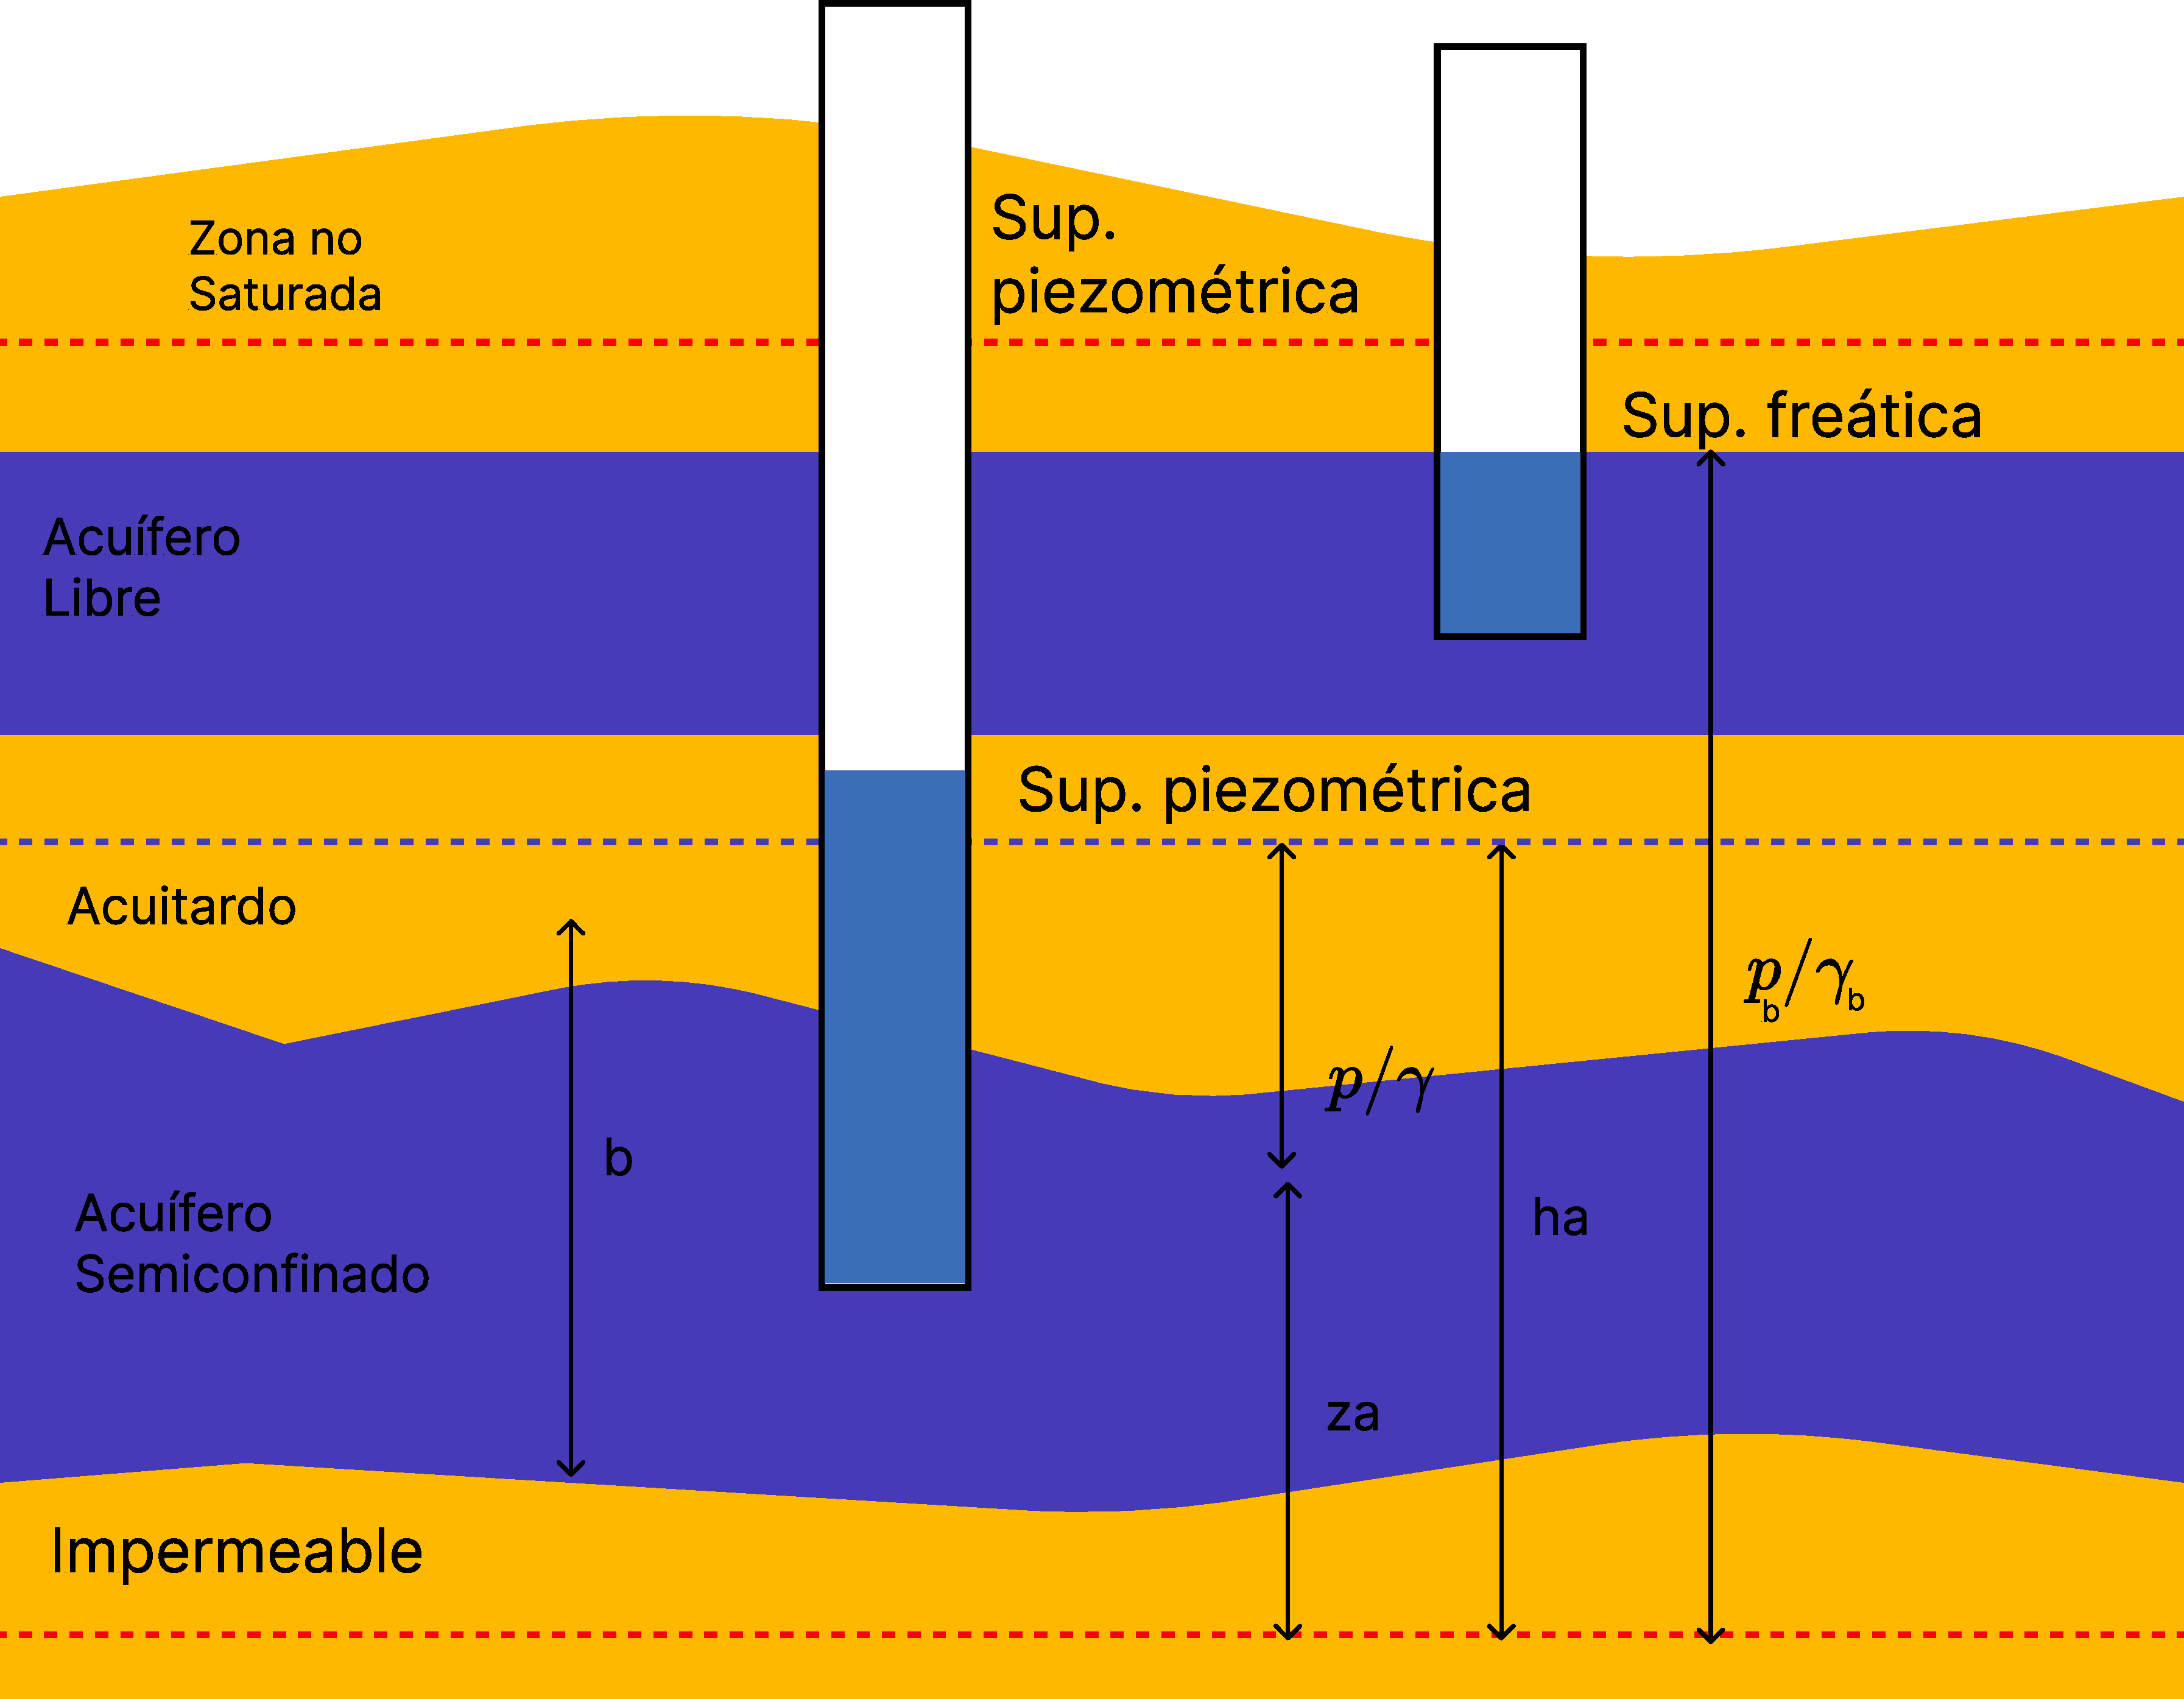
\includegraphics[width=0.5\textwidth]{gh10.pdf}
  \caption{Acuífero semiconfinado}
  \label{gh10}
\end{figure}
\begin{figure}[h!]
\centering
  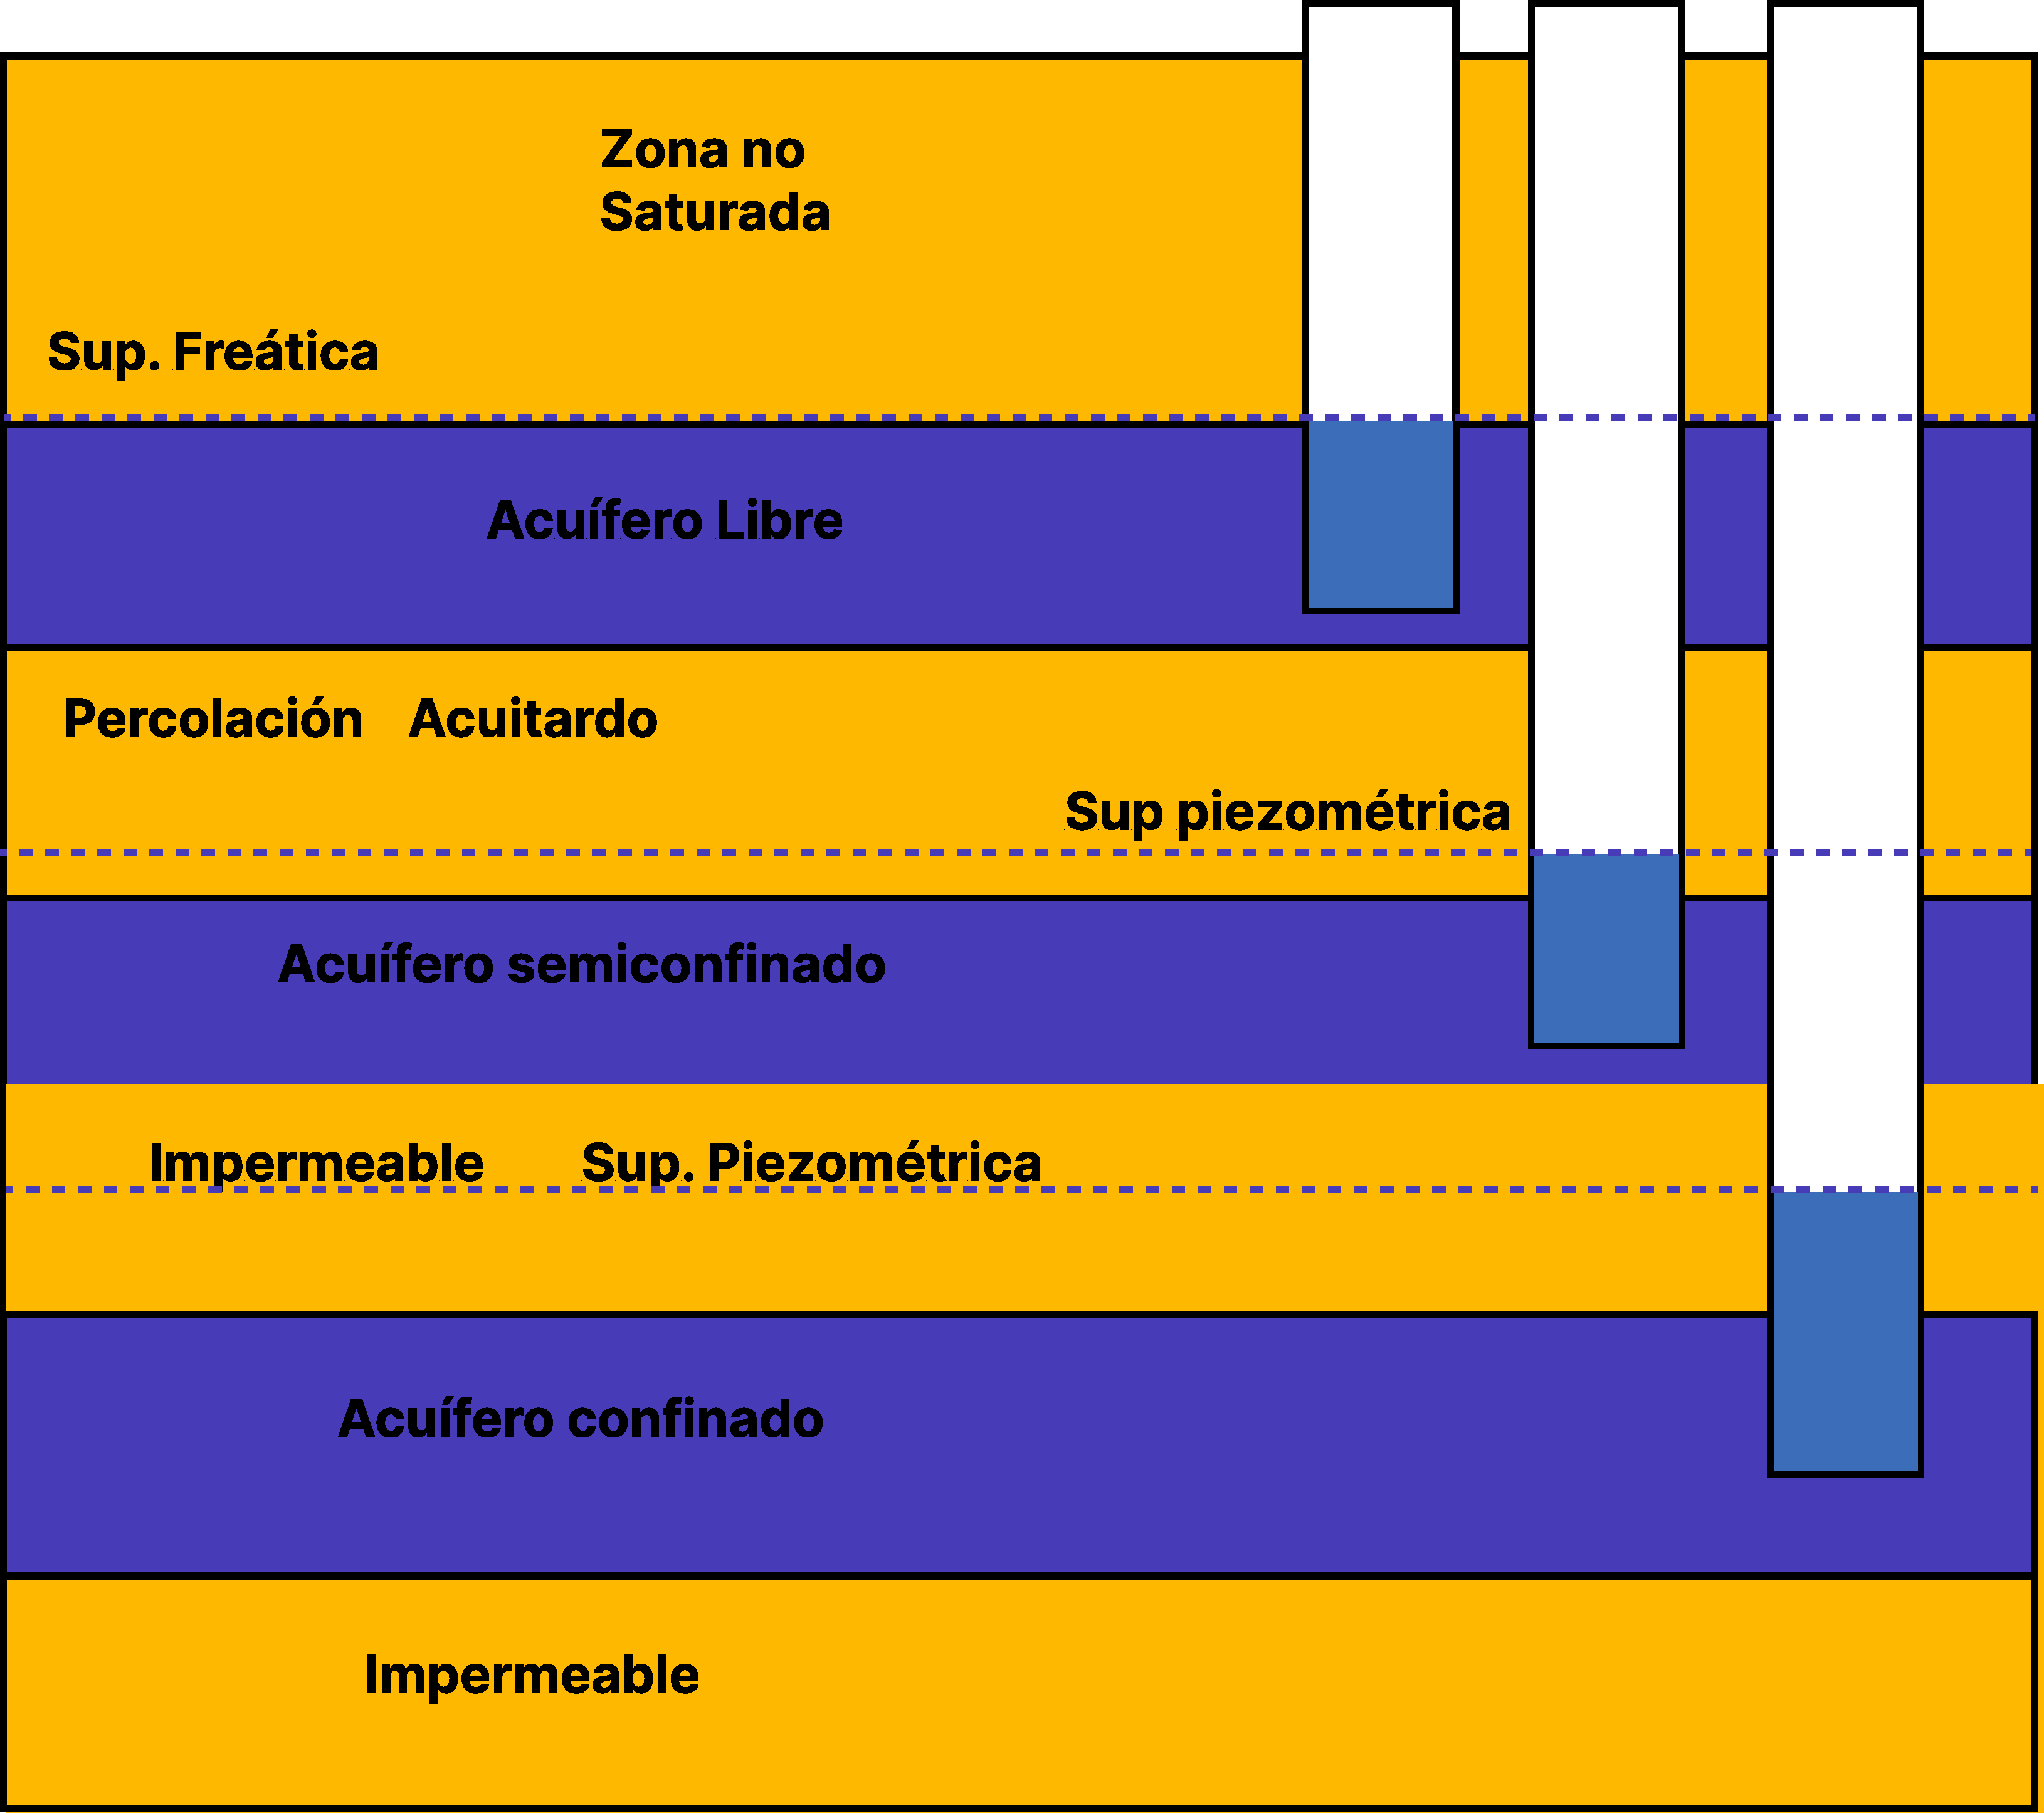
\includegraphics[width=0.5\textwidth]{gh11.pdf}
  \caption{Presentación de los tres tipos de acuíferos}
  \label{gh11}
\end{figure}
\subsection{Coeficiente de almacenamiento}
La capacidad de los acuíferos para almacenar y para transmitir el agua son las características hidráulicas más importantes de un acuífero.
El Coeficiente de almacenamiento (S) es definido como el volumen de agua que un acuífero libera por unidad de área por unidad de cambio en la carga. El coeficiente de almacenamiento no tiene dimensiones. La magnitud del coeficiente de almacenamiento depende en gran medida del tipo de acuífero
\begin{equation}
    S = S_s \cdot b + S_y
\end{equation}
Donde SS es el coeficiente de almacenamiento específico 
\begin{equation}
    S_s = 3.3 \times 10^{- 6}\frac{m^3}{m^3} / m
\end{equation}    
Cuando el acuífero es de tipo libre, la fuente predominante de agua es el drenado por gravedad de los materiales, por el efecto del abatimiento del nivel freático, así en este tipo de acuífero, el coeficiente de almacenamiento es virtualmente igual al rendimiento específico y el rango aproximado de sus valores es de 0.05 a 0.3
% \begin{example}
%     \begin{equation*}
%         V_{agua} = S_{sb} + S_y =3.3 \times 10^{ -6}(50m) + 0.15
%     \end{equation*}
% \end{example}
En un acuífero confinado no existe el $S_y$, la expansión de un volumen dado de agua en respuesta a la baja presión es muy pequeña. Para determinar el coeficiente de almacenamiento en un acuífero debido a la expansión del agua es necesario multiplicar tal expansión por el espesor del acuífero ($S=S_s\cdot b$) $S_s=3.3\times  m^{-1}$.

El coeficiente de almacenamiento de los acuíferos confinados se encuentra dentro del rango $10^{-5}-10^{-3}$, la diferencia entre estos valores y los debidos a la expansión dela gua es atribuida a la compresión del acuífero. El peso total de la capa confinante, es soportado por el esqueleto sólido y por la presión hidráulica en el acuífero. cuando el espesor saturado deja de estar en contacto con el lecho, la carga total es soportada únicamente por el esqueleto sólida, como resultado, las partículas rocosas son deformadas y el espacio rocosos se reduce, llegando a hacer esto de tal magnitud que lleguen a presentarse en la superficie del suelo asentamientos u grietas de tamaño considerable.

Cuando el nivel del agua de un acuífero confinado pierde contacto con la capa confinante, el coeficiente de almacenamiento se incrementa inmediatamente y funciona en condición libre.
\begin{table}[h!]
    \centering
    \begin{tabular}{@{}ccc@{}}
    \toprule
    Acuífero       & Fórmula  & Rango                                                 \\ \midrule
    Libre          & S        & 0.05-0.3                                              \\
    Confinados     & $S=S_sb$ & $10^{-5}-10^{-3}$ \\
    Semiconfinados & S        & $10^{-3}$-0.05                       \\ \bottomrule
    \end{tabular}
    \caption{Rangos de S}
    \label{tabgh4}
\end{table}
\subsection{Mecanismos de recarga y descarga de acuíferos}
De forma natural, los mecanismos de recarga son por:
\begin{enumerate}
    \item la infiltración directa de la lluvia en la superficie y a través de los lechos de los ríos influentes (Cuando la dirección del flujo del agua es hacia el acuífero), lagos y lagunas
    \item Por deshielo
    \item Flujo subterráneo
\end{enumerate}
Los mecanismos artificiales de recarga son por:
\begin{enumerate}
    \item Pozos de absorción
    \item Lechos de absorción
    \item Canales no revestidos, drenes o presas
    \item Láminas excesivas de riego
    \item Fugas en las redes de distribución y drenaje
\end{enumerate}
Los mecanismos de descarga naturales son:
\begin{enumerate}
    \item Evapotranspiración directa de acuíferos libres someros y cenotes
    \item Manantiales
    \item Ríos efluentes
    \item Flujo subterráneo en acuíferos costeros
\end{enumerate}
artificiales
\begin{enumerate}
    \item Bombeo de pozos, norias, cenotes y aguas subálveas
    \item Galerías filtrantes.
\end{enumerate}
\section{Hidrogeología}
\begin{definition}[Hidrogeología]
    Estudio de las aguas subterráneas cuyo énfasis especial recae sobre su circulación y circunstancias geológicas condicionantes, y su aspecto químico. (Davis y De Wiest, 1966). 
\end{definition}
Estudio geológico: Definir la distribución horizontal y vertical de las distintas unidades de roca, para realizar un modelo tridimensional del subsuelo.

Estudio Hidrogeológico: Localizar las partes que se encuentran saturadas de agua, estableciendo su distribución o la variación de la carga hidráulica, para describir la dirección y magnitud del flujo dentro del modelo geológico tridimensional.

La ocurrencia y movimiento del agua subterránea está en función de:
\begin{itemize}
    \item Clima.
    \item Naturaleza de las rocas que forman la región.
    \item Secuencia y distribución de los diferentes tipos de rocas (estratigrafía)
    \item Topografía y geomorfología de la región.
\end{itemize}

Rocas con posibilidades acuíferas:
\begin{itemize}
    \item Las rocas porosas: Incoherentes como las gravas y las arenas, o coherentes (rocas compactas), como las areniscas y las tobas. (Sedimentarias)
    \item Las rocas fisuradas: Son rocas coherentes o compactas, las que sus principales vacíos están esencialmente constituidos por fisuras. (Metamórficas e ígneas)
\end{itemize}
\begin{table}[h!]
    \centering
    \begin{tabular}{@{}cc@{}}
    \toprule
    \begin{tabular}[c]{@{}c@{}}Permeabilidad\\ Máxima\end{tabular} & \begin{tabular}[c]{@{}c@{}}Porosidad\\ Máxima\end{tabular} \\ \midrule
    Gravas                        & Arcillas            \\
    Basalto poroso                & Limos               \\
    Caliza carstificada           & Tobas               \\
    Arenas                        & Arenas              \\
    Rocas cristalinas fracturadas & Gravas              \\
    Limos y tobas                 & Basalto poroso      \\
    Arcillas                      & Caliza carstificada \\
    Rocas cristalinas             & Roca cristalina     \\
    Mínima                        & Mínima              \\ \bottomrule
    \end{tabular}
    \caption{Propiedades acuíferas de algunas rocas comúnes}
    \label{tabgh5}
\end{table}
\begin{figure}[h!]
\centering
  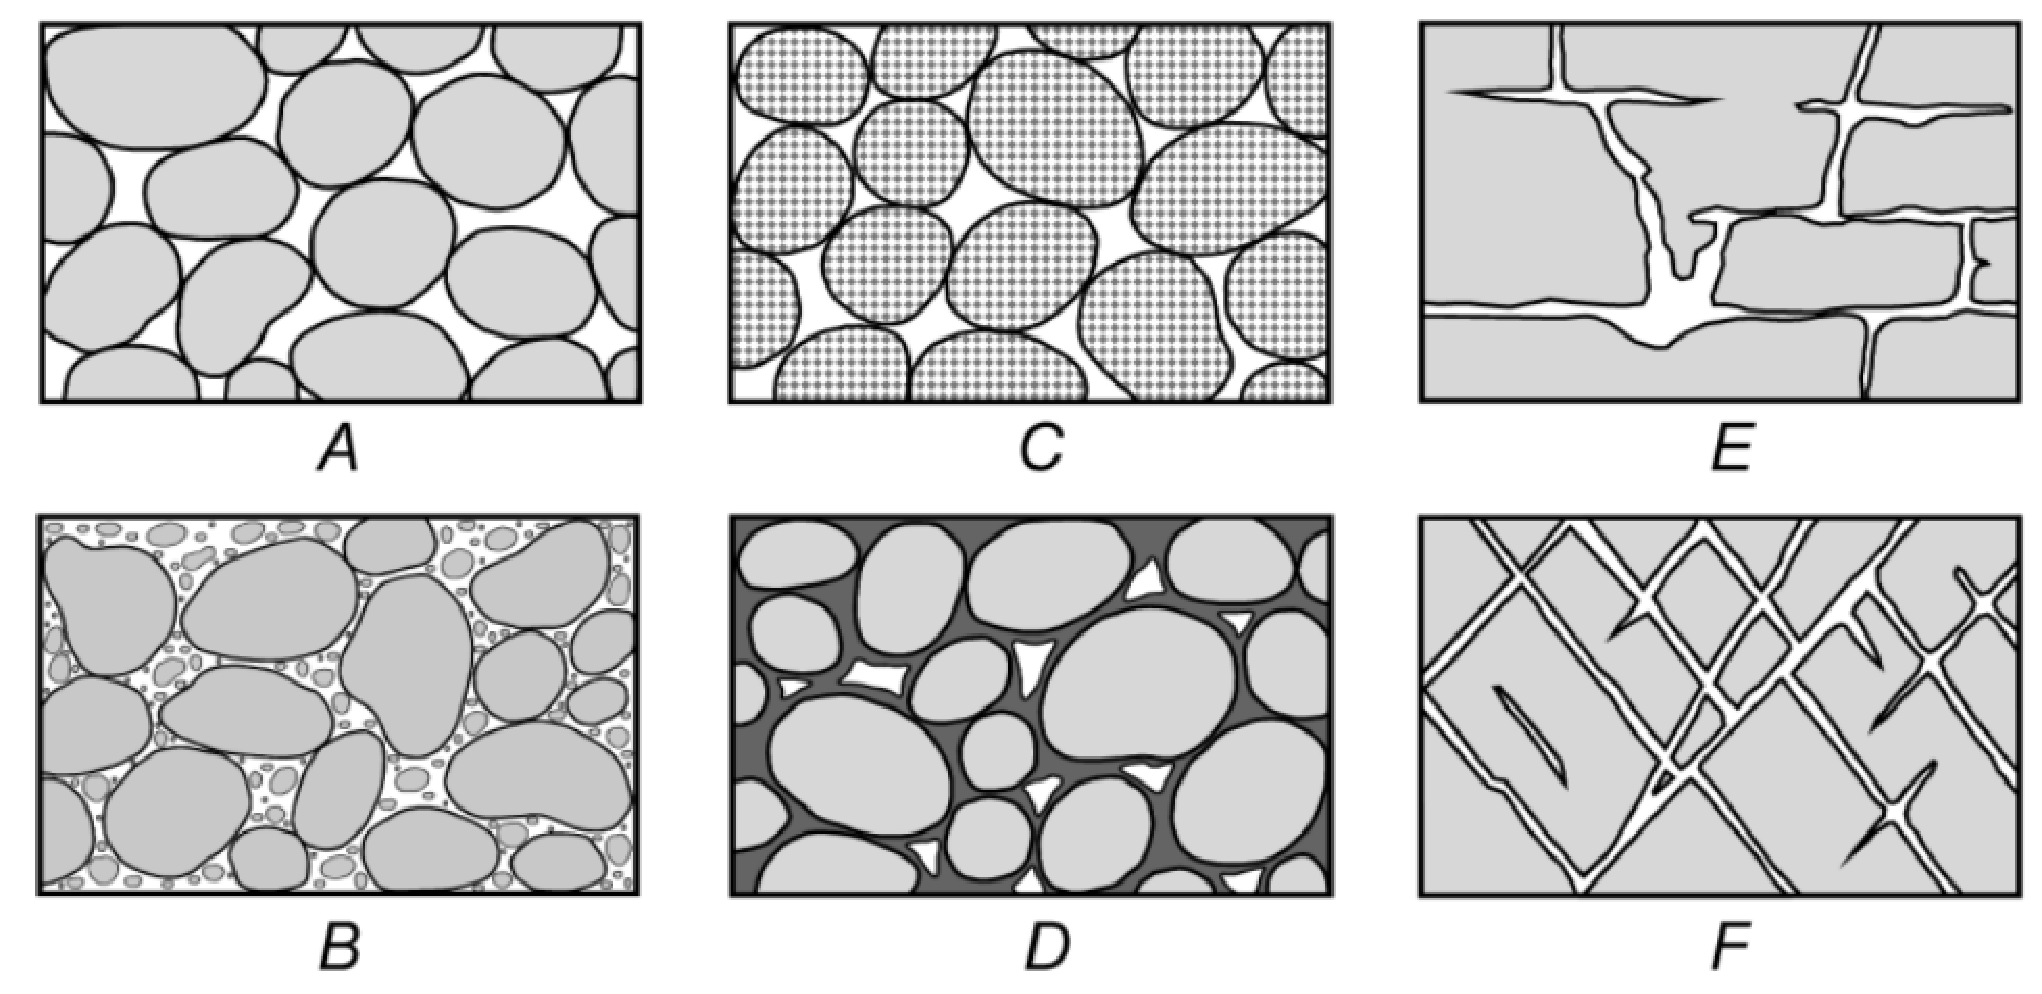
\includegraphics[width=0.6\textwidth]{gh13.pdf}
  \caption{Diagrama que muestra varios tipos de intersticios de roca y la relación entre la textura de la roca y la porosidad. A: depósito sedimentario bien clasificado que tiene alta porosidad; B: depósito sedimentario mal clasificado y de baja porosidad; C: depósito sedimentario bien clasificado que consta de guijarros que son en sí mismos porosos, de modo que el depósito en su conjunto tiene una porosidad muy alta; D: depósito sedimentario bien clasificado cuya porosidad ha sido disminuida por la deposición de materia mineral en los intersticios; E: roca hecha porosa por solución; F, roca hecha porosa por fracturamiento. Modificado de Meinzer, 1923a. USGS, en dominio público.}
  \label{gh13}
\end{figure}
El agua subterránea en los diferentes tipos de rocas:

\subsection{El agua subterránea en las diferentes tipos de rocas}
\subsubsection{Ígneas y metamórficas}

sin alteración (sanas):
\begin{itemize}
\item Porosidad inferior a 3\%
\item Poros pequeños, escasos y por lo general sin conexión entre si
\item →Permeabilidad muy pequeña prácticamente nula.
\end{itemize}
Alteradas (con fracturamiento):
\begin{itemize}
    \item Importante porosidad.
    \item Permeabilidad hasta varios cientos de metros por día en el caso de rocas muy fracturadas.    
\end{itemize}
\subsubsection{Sedimentarias}
ROCAS DETRÍTICAS DE GRANO FINO (50\%), ARENISCAS (48\%) Y ROCAS CARBONATADAS (2\%)
\begin{itemize}
    \item Rocas de grano fino: Porosidad elevadas, permeabilidad muy baja.
    \item Areniscas: Porosidad entre el 10 y 20\%. La
    permeabilidad 10-8 a 1.5x10-3 m/s.
    \item Rocas carbonatadas: Porosidad entre 4 y 30\%.\footnote{La permeabilidad de este tipo de rocas puede variar desde 1 mm por día, en el caso de las calizas compactas ricas en arcilla, hasta varios miles de metros por día}
\end{itemize}
\subsection{Formaciones acuíferas en México}
\begin{itemize}
    \item Aluviones recientes.
    \item Cuencas terciarias continentales y marinas
    \item Calizas cretácicas y terciarias.
\end{itemize}
\subsubsection{Aluviones recientes}
Estos aluviones están constituidos por mantos de gravas, arenas y arcillas que fueron depositadas por las descargas de materiales acarreados por ríos y arroyos, en su desembocadura hacia valles y planicies de inundación. Los acuíferos de este tipo de formación se localizan en las planicies costeras del Océano Pacífico, de los Golfos de California, Tehuantepec y de México. Los lugares donde están siendo explotados, son principalmente los siguientes:
\begin{itemize}
    \item Depósitos Deltáicos del Valle de Mexicali, B. C. N.
    \item Planicies de inundación de Cd. De Obregón, Son.; La paz B. C. S.; Bajo Río bravo, Tamps.; Coatzacoalcos, Ver.
    \item Cuencas cerradas en la Región Lagunera de Coahuila y Durango, cuenca del Valle de México y los Valles centrales de Oax.
\end{itemize}
\subsubsection{Acuíferos en cuencas terciarias} 
\begin{itemize}
    \item Terciario Continental. Gruesos espesores de sedimentos lacustres y aluviales, dentro de lo que es hoy la meseta central y en la región noroeste del país. Debido a la gran actividad volcánica ocurrida en ese tiempo, es común encontrar ese tipo de sedimentos, intercalados con derrames de rocas ígneas y depósitos piroclásticos. Algunos de los acuíferos en explotación, se encuentran en Nuevo Casas Grandes Chih.; Vicente guerrero Dgo.; Noria de Ángeles Zac.; Valle de Aguascalientes, Tequisquiapan Qro. y Acámbaro Gto.
    \item Terciario Marino. La mayoría de ellas formada por mantos de arcillas, arenas y materiales calcáreos, siendo algunas de ellas productoras de agua de buena calidad.
    
    Algunos ejemplos de acuíferos que se explotan en éste tipo de formación son: Minatitlán Ver., Jalpa Tab., Desde Poza rica Ver. hasta Matamoros Tamps., Valle de Misión, San quintín, Vizcaíno y Santo Domingo en B.C.
\end{itemize}
\subsubsection{Acuíferos en Calizas}
\begin{itemize}
    \item Constituidas principalmente por carbonatos de calcio. Calizas cretácicas son formadoras de la Sierra Madre Oriental, parte de la Sierra Madre del Sur y Sierra de Chiapas.
    \item La explotación de esta formación con gran potencial acuífero, se inició en Monterrey N. L., con perforaciones que han alcanzado profundidades hasta de 2000 metros, pero con niveles de bombeo someros o inclusive como pozos brotantes.
    \item La península de Yucatán está formada por una secuencia de mantos calcáreos de origen marino del cretácico hasta el terciario, en la que afloran exclusivamente calizas, que son acuíferos de muy alto potencial productor, explotadas en Mérida, Ticul y Peto en Yucatán; Cancún, Pucté y Álvaro Obregón en Quintana Roo y Edzná y Champotón en Campeche.
\end{itemize}
\subsection{Prospección hidrogeológica}
La prospección o exploración, tiene por objeto la localización de los acuíferos, y la definición de su naturaleza y dimensiones.

Además del estudio de aspectos hidrológicos y geológicos, que pueden proporcionar una idea cualitativa de la disponibilidad de agua subterránea, como vegetación, red hidrográfica, manantiales, características hidrogeológicas de las rocas, otros.

Para obtener la información señalada se requiere de planos geológicos, de reconocimientos y exploración hidrogeológica, esto es exploraciones subterráneas directas (pozos exploratorios) e indirecta (sondeos geofísicos).

\begin{figure}[h!]
\centering
  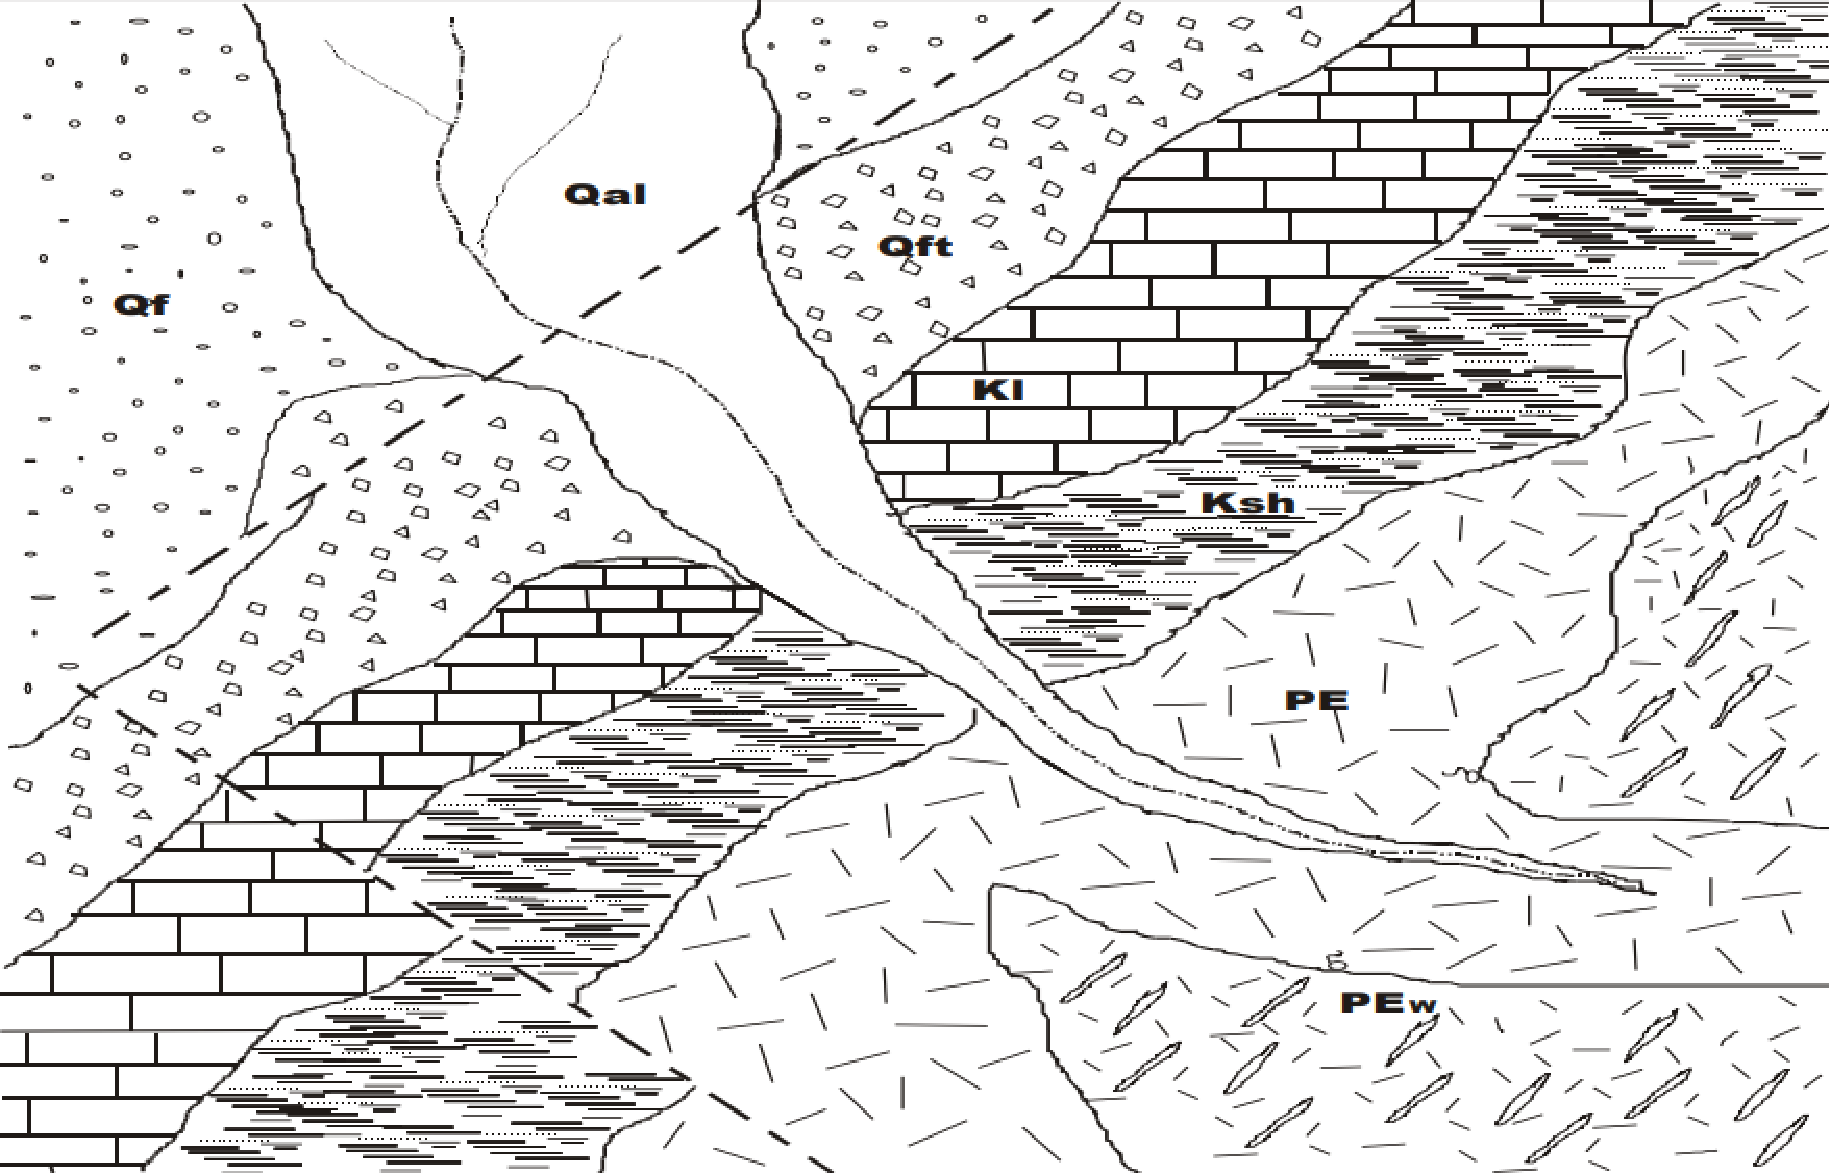
\includegraphics[width=0.8\textwidth]{gh12.pdf}
  \caption{Plano Hidrogeológico}
  \label{gh12}
\end{figure}
Plano hidrogeológico
\begin{itemize}
    \item $Qal$: Aluviones recientes 1.5 a 7m de espesor parcialmente saturados
    \item $Qt$ Cono aluvial 7 a a 130 m de espesor. Acuífero regional principal
    \item $Q_{ft}$: Aluviones antiguos y cono aluvial, 3 a 100m de espesor
    \item $Kl$ Caliza masiva de baja permeabilidad, no se supone acuífera
    \item $K_{sh}$: Arcilla y limonita impermeables
    \item $PE_{w}$: Granito y genesis precámbricos, 1.5 a 15m de espesor alterado localmente es acuífero
    \item $PE$: Granito y génesis no alterados
    \item Manantial
    \item Falla
\end{itemize}

\subsection{Métodos indirectos de exploración}
La Geofísica es una rama de la física aplicada que se
ocupa del estudio de las estructuras ocultas (del
interior) de la tierra y de la localización en ésta, de
cuerpos delimitados por el contraste de alguna de sus
propiedades físicas con las del medio circundante,
mediante observaciones realizadas en la superficie.
(Orellana, 1972)
Algunas de las aplicaciones más comunes:
\begin{itemize}
    \item Estudios para la localización de agua subterránea.
    \item Investigaciones tectónicas para la búsqueda de petróleo.
    \item Estudio para investigaciones Geológicas.
    \item Estudios para la localización y cubicación de materiales de construcción.
    \item Estudios de cimentaciones para ingeniería civil.
    \item Localización de minerales diversos.
\end{itemize}
Métodos geofísicos:
\begin{itemize}
    \item Campo natural \begin{itemize}
        \item Método gravimétrico
        \item Método magnético
    \end{itemize}
    \item Campo artificial \begin{itemize}
        \item Método eléctrico
        \item Método sísmico
    \end{itemize}
    \item Eléctrico resistivo
    \item Sísmico de refracción
    \item Gravimétrico
\end{itemize} 
\subsection{Método eléctrico resistivo}

\begin{definition}[Resistividad $(\rho)$]
    Cualitativamente, la resistividad es una medida de la dificultad que la corriente eléctrica encuentra a su paso por un material determinado.
    
    La resistividad ($\rho$) es numéricamente igual a la Resistencia que opone un cubo de dicho material, al paso de una corriente eléctrica que circula en dirección perpendicular a dos de sus caras entre las cuales existe una diferencia unitaria de potencial (Camarena, 1976)
\end{definition}

Ley de Ohm, la cual establece que la caída de potencial ($\Delta V$),
es proporcional a la intensidad de corriente eléctrica ($I$)
que circula por un conductor, multiplicada por una constante de
proporcionalidad ($R$) llamada resistencia.
\begin{equation}
    \Delta V = RI
\end{equation}

R es una propiedad intrínseca de los materiales puesto que
depende de las dimensiones del conductor.

De física se conoce que la resistencia de un conductor alargado y
homogéneo de forma cilíndrica o prismática vale:
\begin{equation}
    R = \rho\frac{l}{s}
\end{equation}
\begin{notation}
    \begin{itemize}
        \item $l$ es arista o generatriz del conductor.
        \item $s$ es el área de la sección transversal.
        \item $\rho$ es resistividad.
    \end{itemize}
\end{notation}
Por lo que la resistividad será:
\begin{equation}
    \rho = R\frac{s}{l}
\end{equation}
Factores de mayor importancia que
influyen en la resistividad de las rocas:
\begin{itemize}
    \item Constitución mineralógica.
    \item Grado de saturación y calidad del agua saturante.
    \item Porosidad
    \item Grado de compactación
\end{itemize}
\begin{figure}[h!]
\centering
  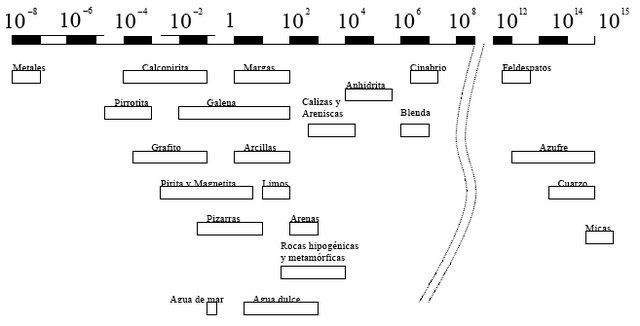
\includegraphics[width=0.8\textwidth]{gh15.jpg}
  \caption{Gráfica de los márgenes de variación más comunes en algunas rocas y minerales. La fisuración, impregnación de agua salada, etc. pueden extender estos límites. (Orellana 1972)}
  \label{gh15}
\end{figure}
\subsection{Dispositivos fundamentales en la prospección eléctrica por corriente continua.}
\begin{definition}[Resistividad aparente ($\rho_a$)]
    Es la resistividad ficticia que se obtiene aplicando a los datos obtenidos sobre un medio heterogéneo, la expresión correspondiente a medio homogéneo (Orellana, 1972). Esta es la variable experimental que expresa los resultados  de las mediciones en la mayoría de los métodos geoeléctricos y la que se toma como base para la interpretación.
\end{definition}
\begin{definition}[Electródos]
    Son las barras metálicas que se utilizan para inyectar la corriente eléctrica al terreno (electrodos de corriente) y para dividir el cambio de potencial que se genera por la influencia del perfil de estudio (electrodos de potencial)
\end{definition}
Determinación del potencial eléctrico V a una distancia r de un electrodo de corriente A en un medio semi-finito, homogéneo e isótropo.
\begin{figure}[h!]
\centering
  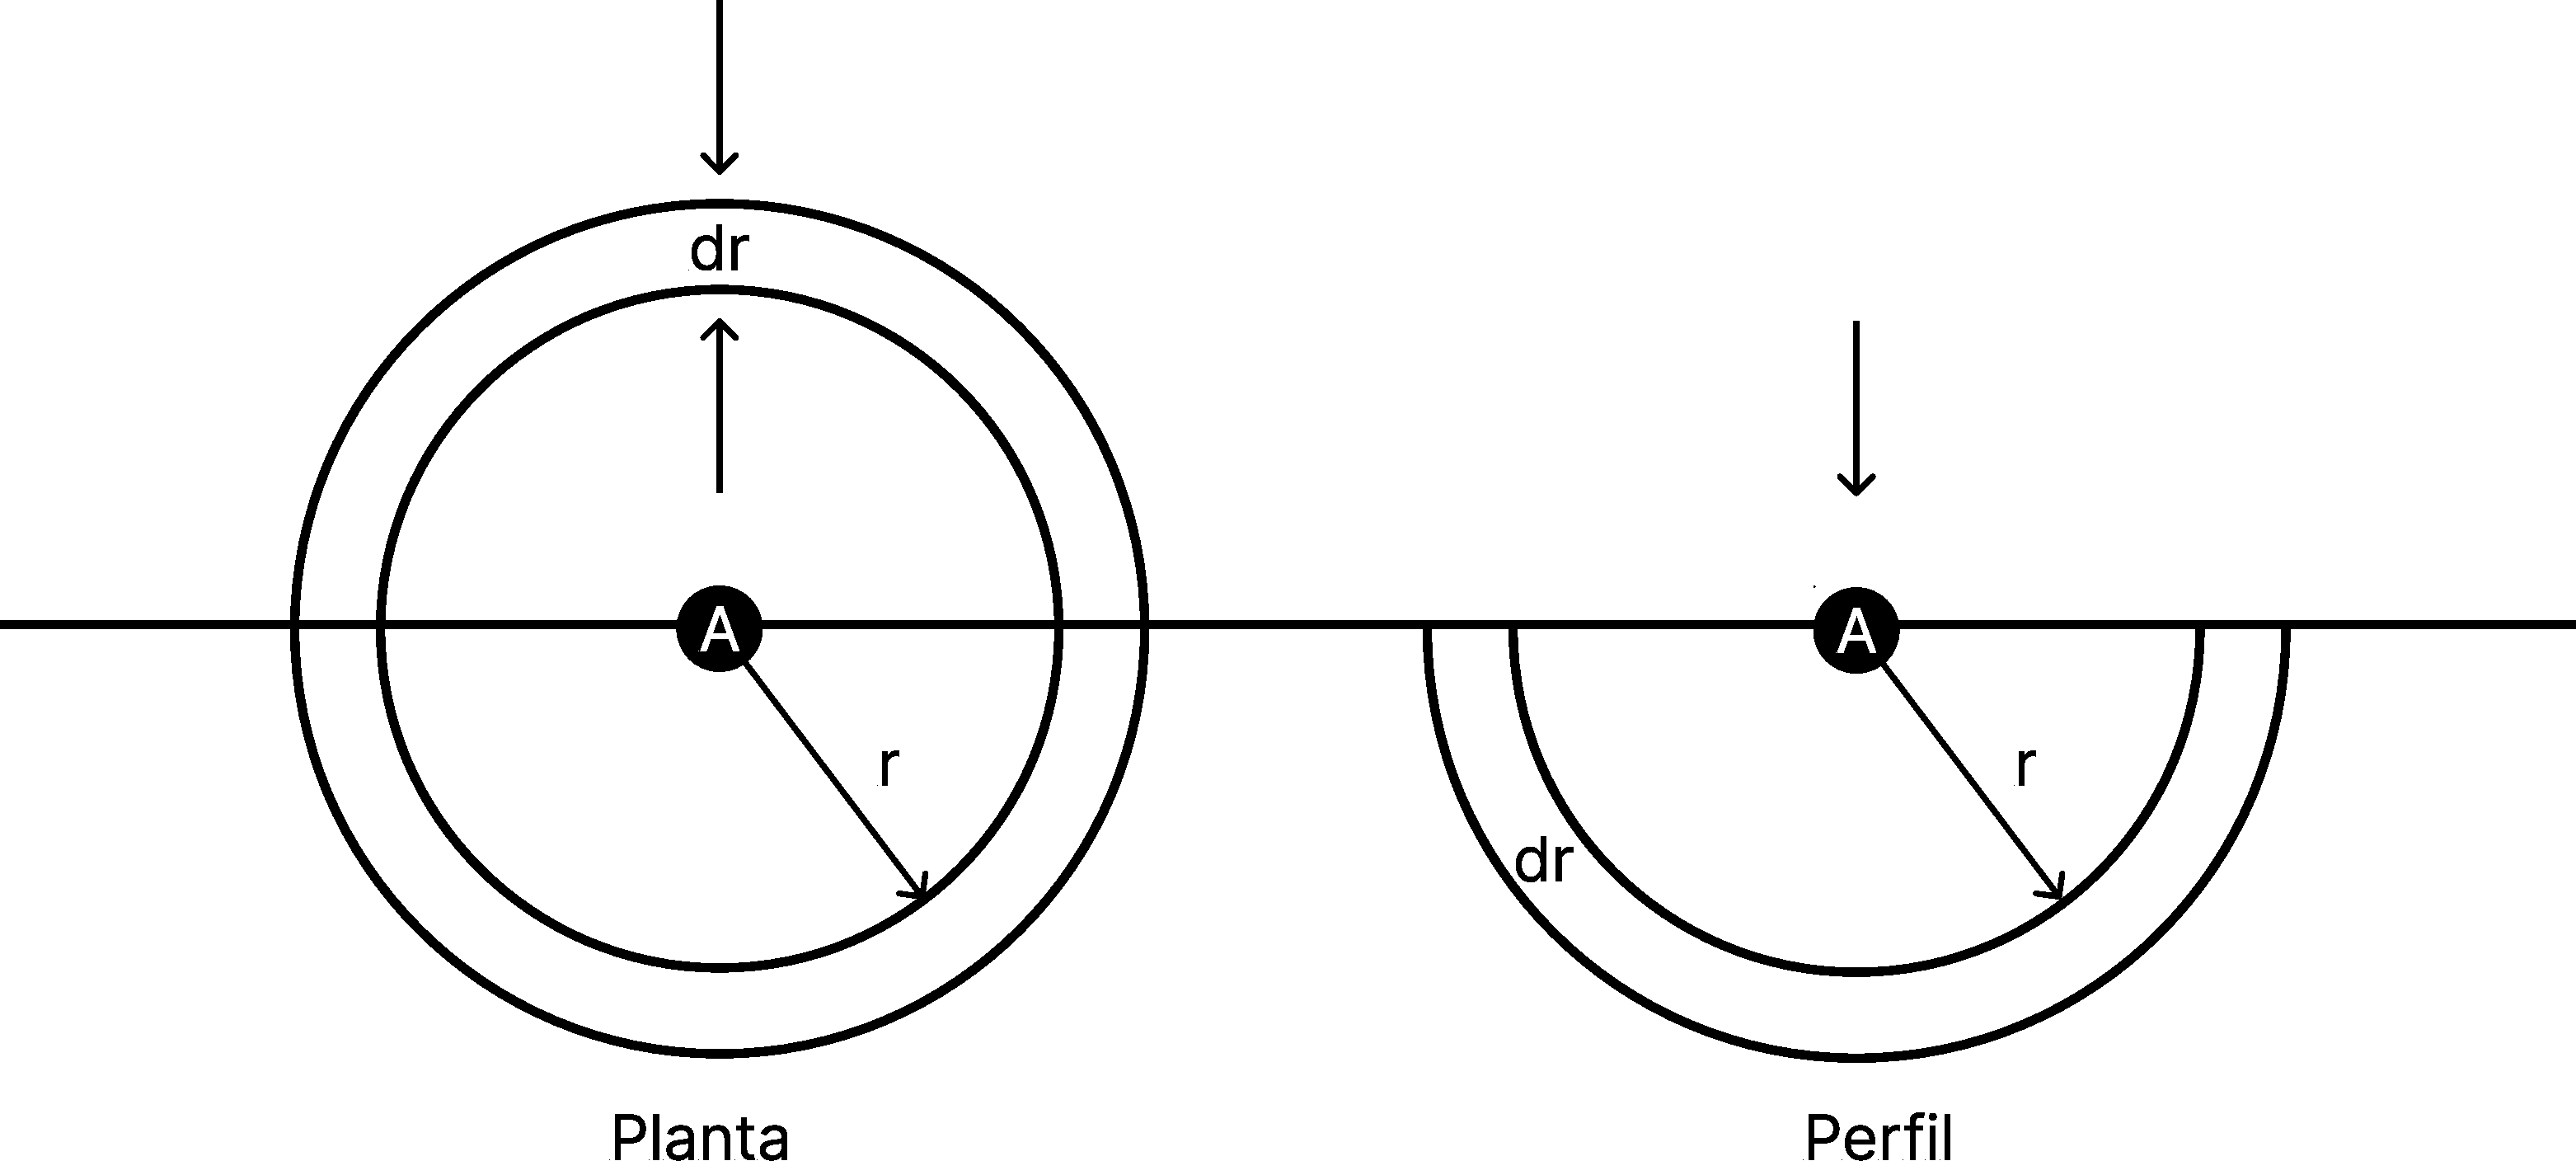
\includegraphics[width=0.8\textwidth]{gh14.pdf}
  \caption{Semi-esfera generada por la corriente eléctrica inyectada en un medio homogéneo e isótropo.}
  \label{gh14}
\end{figure}
A una distancia r del electrodo A se tiene un elemento diferencial de dimensiones dr. La resistencia eléctrica que presenta el elemento diferencial al paso de la corriente I es dR, que según la ley de Ohm.
\begin{equation}
    dR = \frac{dV}{I}
\end{equation}
También se tiene que:
\begin{equation}
    dR = \rho \frac{dr}{s}
\end{equation}
Para la esfera de radio r, el área transversal al flujo de la corriente es la superficie de la esfera. Como la atmósfera presenta resistividad infinita, se considera sólo la media esfera definida por el terreno. Para la semiesfera, la superficie es $S=2\pi r^2$, igualando y sustituyendo S, se tiene:
\begin{align*}
    &\rho = \frac{dr}{2\pi r^2} = \frac{dV}{I}\\
    &dV = - \frac{\rho I}{2\pi }\frac{dr}{r^2}
\end{align*}
En donde el signo negativo, indica que a medida que crece r, el V decrece, así integrando se obtiene:
\begin{align*}
    &\int dV = -\int \frac{\rho I}{2\pi}\frac{dr}{r^2}\\
    &V =\frac{\rho I}{2\pi r}
\end{align*}
Esta última ecuación es la que define el campo eléctrico generado al aplicar corriente eléctrica al subsuelo, mediante electrodos, bajo el supuesto de que la aplicación es puntual. Definidas las líneas equipotenciales se pueden trazar las líneas de corriente ortogonales entre ellas.

\subsection{Dispositivos electródicos}
Hasta ahora, se ha mencionado el uso de los electrodos de corriente y de potencial, sin especificar la relación geométrica entre ellos. A continuación se indican las disposiciones más comunes que se utilizan en la actualidad, así como sus características.

Se le denomina dispositivo electródico, configuración electródica o arreglo electródico, a la disposición geométrica que existe entre los electrodos

\begin{equation}
  \rho_a = K\cdot \frac{\Delta V}{I}
\end{equation}
Donde K es un coeficiente que depende únicamente de la geometría del dispositivo (forma del conductor)

Si el medio es Homogéneo, la ecuación anterior determina su resistencia
general en que los cuatro electrodos adoptan una posición cualquiera sore una superficie plana:
\begin{equation}
  K = 2\pi\left(\frac{1}{AM} - \frac{1}{MB} - \frac{1}{AN} + \frac{1}{BN}\right)^{-1}
\end{equation}
Considerando una posición arbitraria de los electrodos
% TODO: Figura Disposición cualquiera de electrodos.

\begin{notation}
  \begin{itemize}
    \item $V_{m}^{AB}$ Potencial en el electrodo M debido a la corriente I de electrodos A y B
    \item $V_{N}^{AB}$ Potencial en el electrodo N debido a la corriente I de electrodos A y B
    \item $V_{M}^{A}$ y $V_{M}^{B}=$ Potencial en electrodo M debido a la corriente I de electrodos A y B respectivamente
    \item $V_{N}^{A}$ y $V_{N}^{B}=$ Potencial en electrodo N debido a la corriente I de electrodos A y B respectivamente.
  \end{itemize}
\end{notation}
Así:
\begin{align}
  V_m^{AB} = V_m^A - V_m^B&& V_N =V_N^A - V_N^B
\end{align}
La diferencia de potencial $\Delta V$ estará dada por:
\begin{equation}
  \Delta V = V_M^{AB} - V_N^{AB} =\left(V_M^A - V_M^B \right) -\left(V_N^A -V_N^{N} \right)
\end{equation}
Utilizando la ecuación del campo eléctrico $V=\frac{\rho I}{2\pi r}$ donde r es la distancia entre electrodos, quedan:
\begin{equation*}
  \Delta V = \left(\frac{\rho I}{2\pi}\frac{1}{AM} -\frac{\rho I}{2\pi}\frac{1}{BM}  \right)
\end{equation*}
Quedando:
\begin{equation}
  K = 2\pi\left(\frac{1}{AM} - \frac{1}{BM} - \frac{1}{AN} + \frac{1}{BN}\right)^{- 1}
\end{equation}

Clasificación:
\begin{itemize}
  \item Lineales \begin{itemize}
    \item Simétricos \begin{itemize}
      \item Schlumberger
      \item Wenner
      \item Lee
    \end{itemize}
    \item Asimétricos \begin{itemize}
      \item Semi-Shlumberger
      \item Semi-Wenner
    \end{itemize}
  \end{itemize}
  \item Dipolares
\end{itemize}
\subsection{Dispositivos electródicos lineales}
Se caracterizan por los cuatro electrodos que los forman se disponen en línea recta. El orden de colocación es A,M,N y B. Los dispositivos lineales se dividen en simétricos y asimétrico.
\begin{figure}[h!]
\centering
  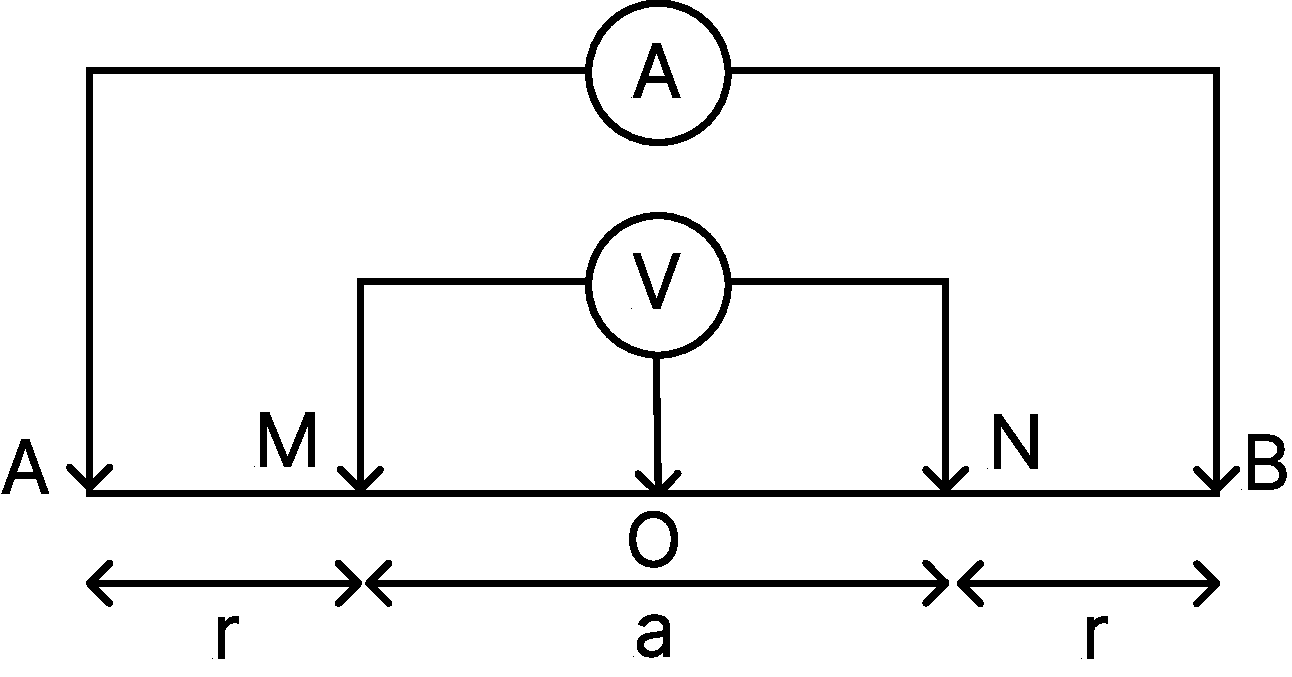
\includegraphics[width=0.5\textwidth]{gh17.pdf}
  \caption{Dispositivos electródicos lineales}
  \label{gh17}
\end{figure}
\subsubsection{Dispositivos simétricos}
En estos los electrodos se disponen simétricamente respecto del centro O. SI hacemos $r=AM=NB$ y $a=MN$, el factor geométrico (K) de estos es:
\begin{align*}
  &K = 2\pi\left(\frac{1}{AM} - \frac{1}{BM} - \frac{1}{AN} + \frac{1}{BN}\right)^{- 1}\\
  &K = 2\pi\left(\frac{1}{r} -\frac{1}{a+ r} - \frac{1}{r+ a} + \frac{1}{r}\right)^{- 1}\\
  &K = 2\pi\left(\frac{2}{r} - \frac{2}{a + r} \right)^{ - 1}\\
  &K = \pi\left(\frac{a + r - r}{r(a + r)}\right)^{ - 1 }\\
  &K = \frac{\pi}{a} \cdot r\left(r + a\right)
\end{align*}
Los dispositivos simétricos más comunes son:
\subsubsection{Dispositivo Schlumberger}
Se caracteriza por que la distancia MN debe ser menor o igual a un quinto de la distancia AB; esto es:
\begin{equation}
  MN\leq \frac{1}{5} AB
\end{equation}
\begin{figure}[h!]
\centering
  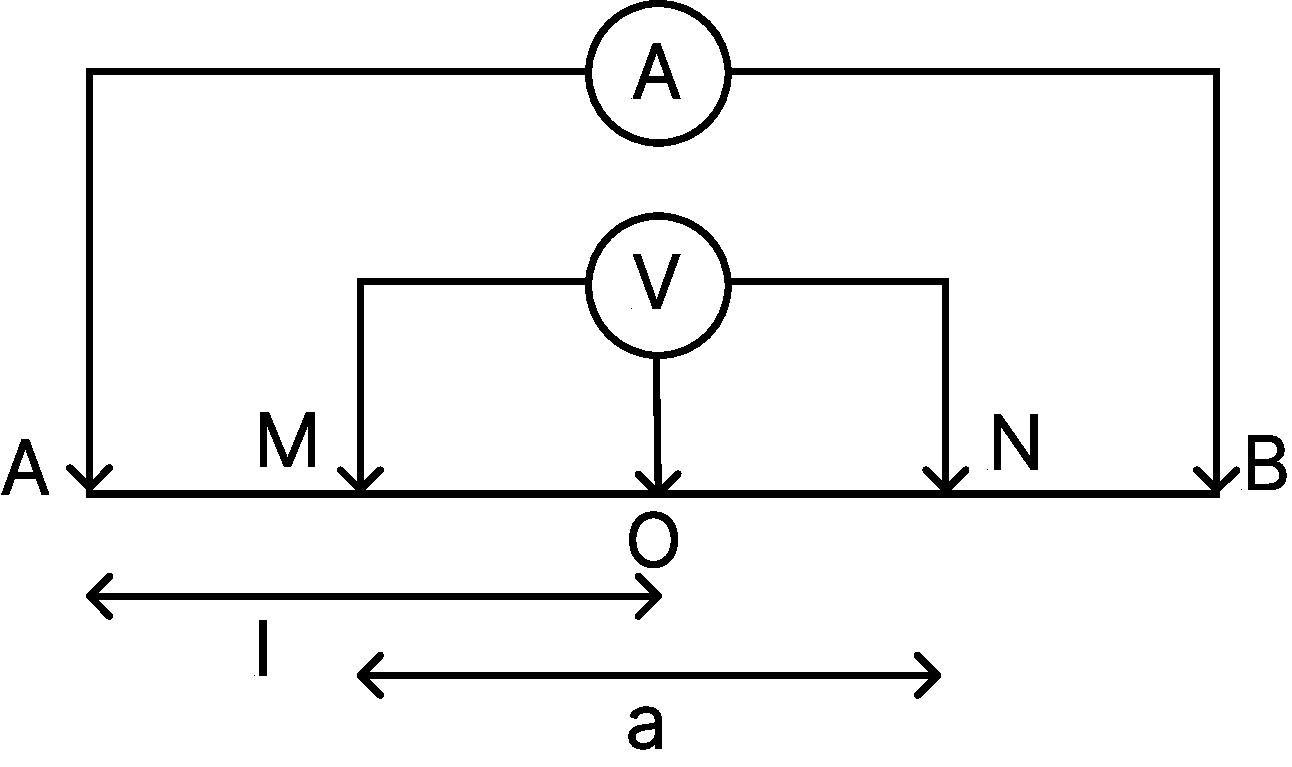
\includegraphics[width=0.5\textwidth]{gh18.pdf}
  \caption{Dispositivo Schlumberger}
  \label{gh18}
\end{figure}
Lo anterior se realiza con la finalidad de que el error que resulta de despreciar la distancia a, sea insignificante. Si $l=AO=BO$, la constante K toma la forma:
\begin{align*}
  &K = 2\pi\left(\frac{1}{AM} - \frac{1}{BM} - \frac{1}{AN} + \frac{1}{BN}\right)^{- 1}\\
  &K = 2\pi\left(\frac{1}{\left(l -\frac{a}{2} \right)} -\frac{1}{\left(l +\frac{a}{2} \right)} -\frac{1}{\left(l +\frac{a}{2} \right)} +\frac{1}{\left(l -\frac{a}{2} \right)}\right)^{- 1}\\
  &K = 2\pi\left(\frac{2}{\left(l -\frac{a}{2} \right)} -\frac{2}{\left(l +\frac{a}{2} \right)}\right)^{ - 1}\\
  &K = \frac{\pi}{a} \left(l^2 - \frac{a^2}{4} \right) =\frac{\pi}{MN}\left[\left(\frac{AB}{2}\right)^2 - \frac{MN^2}{4}\right]
\end{align*}
Por lo tanto:
\begin{equation}
  \rho_a = \frac{\pi}{a}\left(l^2 - \frac{a^2}{4} \right)\frac{\Delta V}{I} = \frac{\pi}{MN}\left[\left(\frac{AB}{2}\right)^2 - \frac{MN^2}{4} \right]\frac{\Delta V}{I}
\end{equation}
donde puede despreciarse $a$, dentro del corchete.
\begin{problem}[Datos]
  \begin{itemize}
    \item AB=120m
    \item MN/2= 3.5m
    \item $\Delta V=289mV$
    \item $I=35.3mA$
  \end{itemize}
\end{problem}
\textit{ Sol. }

K=1610.18m, $\rho_a=13,183.5\Omega m$: Rocas compactas.
\begin{itemize}
  \item $\rho_a=1610.18\cdot 8.187$
  \item $\omega=13,183.5 \Omega m$
\end{itemize}
Despreciando $a^2/4$:
\begin{itemize}
  \item $\rho_a=KR=1615.7\cdot 8.187$
  \item $\omega=13,227.7 \Omega m$
  \item dif(\%)= 0.335\%
\end{itemize}
\begin{table}[h!]
  \centering
  \begin{tabular}{@{}cc@{}}
  \toprule
  \begin{tabular}[c]{@{}c@{}}Resistividad eléctrica\\ $(\Omega m)$\end{tabular} & Probable material                      \\ \midrule
  \textless{}1                                                                  & Materiales con gran contenido de sales \\
  1-10              & Arcillas                    \\
  10-15             & Arcillas arenosas o limosas \\
  15-30             & Arenas arcillosas o limosas \\
  30-60             & Arenas saturadas            \\
  60-100            & Arenas y gravas             \\
  \textgreater{}100 & Rocas                       \\ \bottomrule
  \end{tabular}
  \caption{Valores de resistividad de algunos materiales (CONAGUA, 2007), siempre se buscan rangos cercanos a 30-40, arriba de 100 pueden desarrollar fracturamiento y tener posibilidades de acuífero}
  \label{tabgh6}
\end{table}
\subsubsection{Dispositivo Lee}
Es un caso particular del dispositivo Wenner. Se caracteriza por tener un electrodo adicional (P) en el centro del arreglo, esto permite tomar doble lectura de $\Delta V$. la primera lectura con electrodos MP y segunda lectura con electrodos PN. El factor geométrico de este dispositivo es:
\subsubsection{Dispositivo de Wenner}
Se caracteriza porque la distancia que separa a los electrodos es la misma, esto es AM=MN=NB=a. Bajo esta consideración el factor geométrico de este dispositivo es:
\begin{figure}[h!]
\centering
  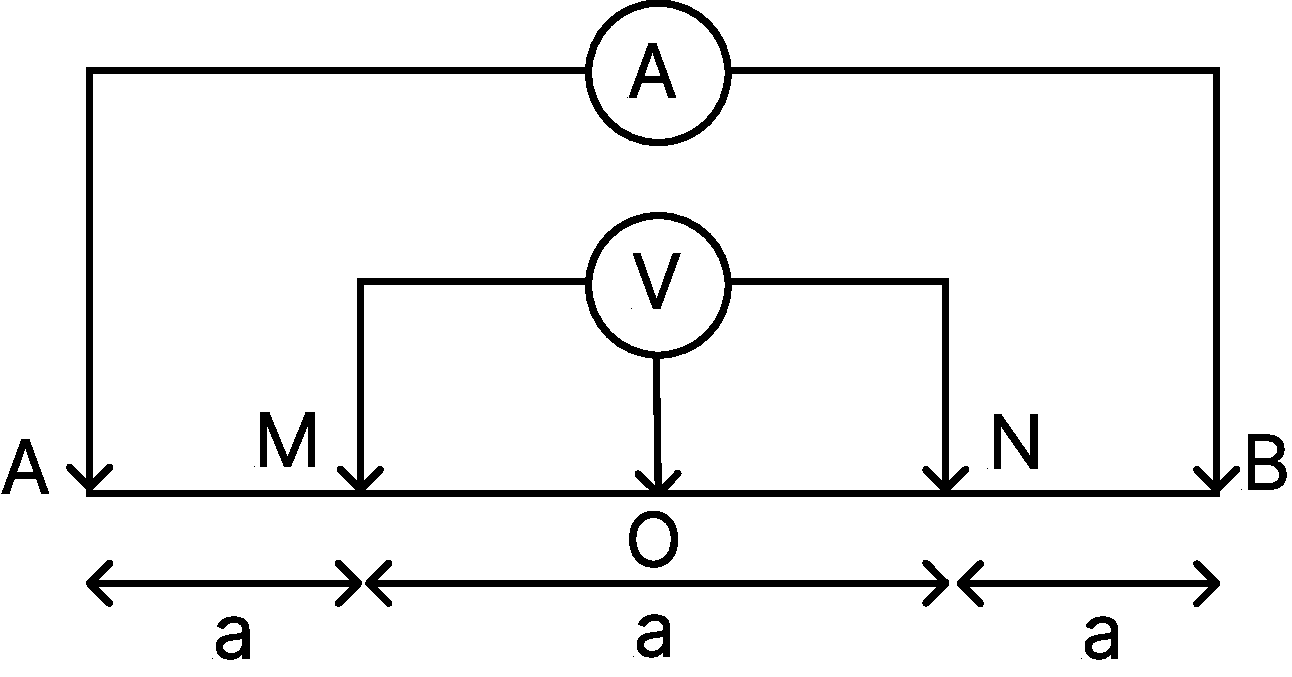
\includegraphics[width=0.5\textwidth]{gh16.pdf}
  \caption{Dispositivo Wenner}
  \label{gh16}
\end{figure}
\begin{problem}[Datos: a=550m $\Delta V= 9.32 mV$, $I=1.62A$, determine:]
  \textit{ Sol. }
\end{problem}
\begin{equation}
  2\pi a
\end{equation}
Datos= a=210m $\Delta V=0.26m$, $I=0.76$. Determine:
\begin{itemize}
    \item $K=1319.47m$
    \item $P=0.45\Omega m$
    \item Material: Con gran contenido de sales.
\end{itemize}
% TODO: VER QUÉ HABíA ANTES

Datos I=700m, a=50m, $\Delta V=1.45mV$, I=1.21, determinar K=61496.82m, y $p=76.69\Omega m$ y es gravas-arenas
\subsubsection{Dispositivo Wenner modificado}
Al igual que el caso anterior, en este dispositivo, un electrodo A o B se manda al infinito. Se deben considerar las mismas observaciones que en el caso anterior, pero con las particularidades que tiene este dispositivo.

En este caso el factor geométrico es:

Datos 25m, $\Delta V=0.06mV$, $I=5mA$, determine K=314.16m, $p=3.77\Omega m$, y material arcilla.
\begin{equation}
    k = 4\pi a
\end{equation}
\subsection{Sondeo eléctrico (SEV)}
Las investigaciones del subsuelo pueden realizarse en dos direcciones
\begin{enumerate}
    \item \textbf{Horizontal:} Esto es paralela a la superficie del terreno, la cual recibe el nombre de ``calcata'' o perfil resistivo, en ella el factor geométrico permanece, 
    dando como resultado información geoeléctrica del subsuelo en dirección horizontal a una determinada profundidad.
    \begin{figure}[h!]
        \centering
        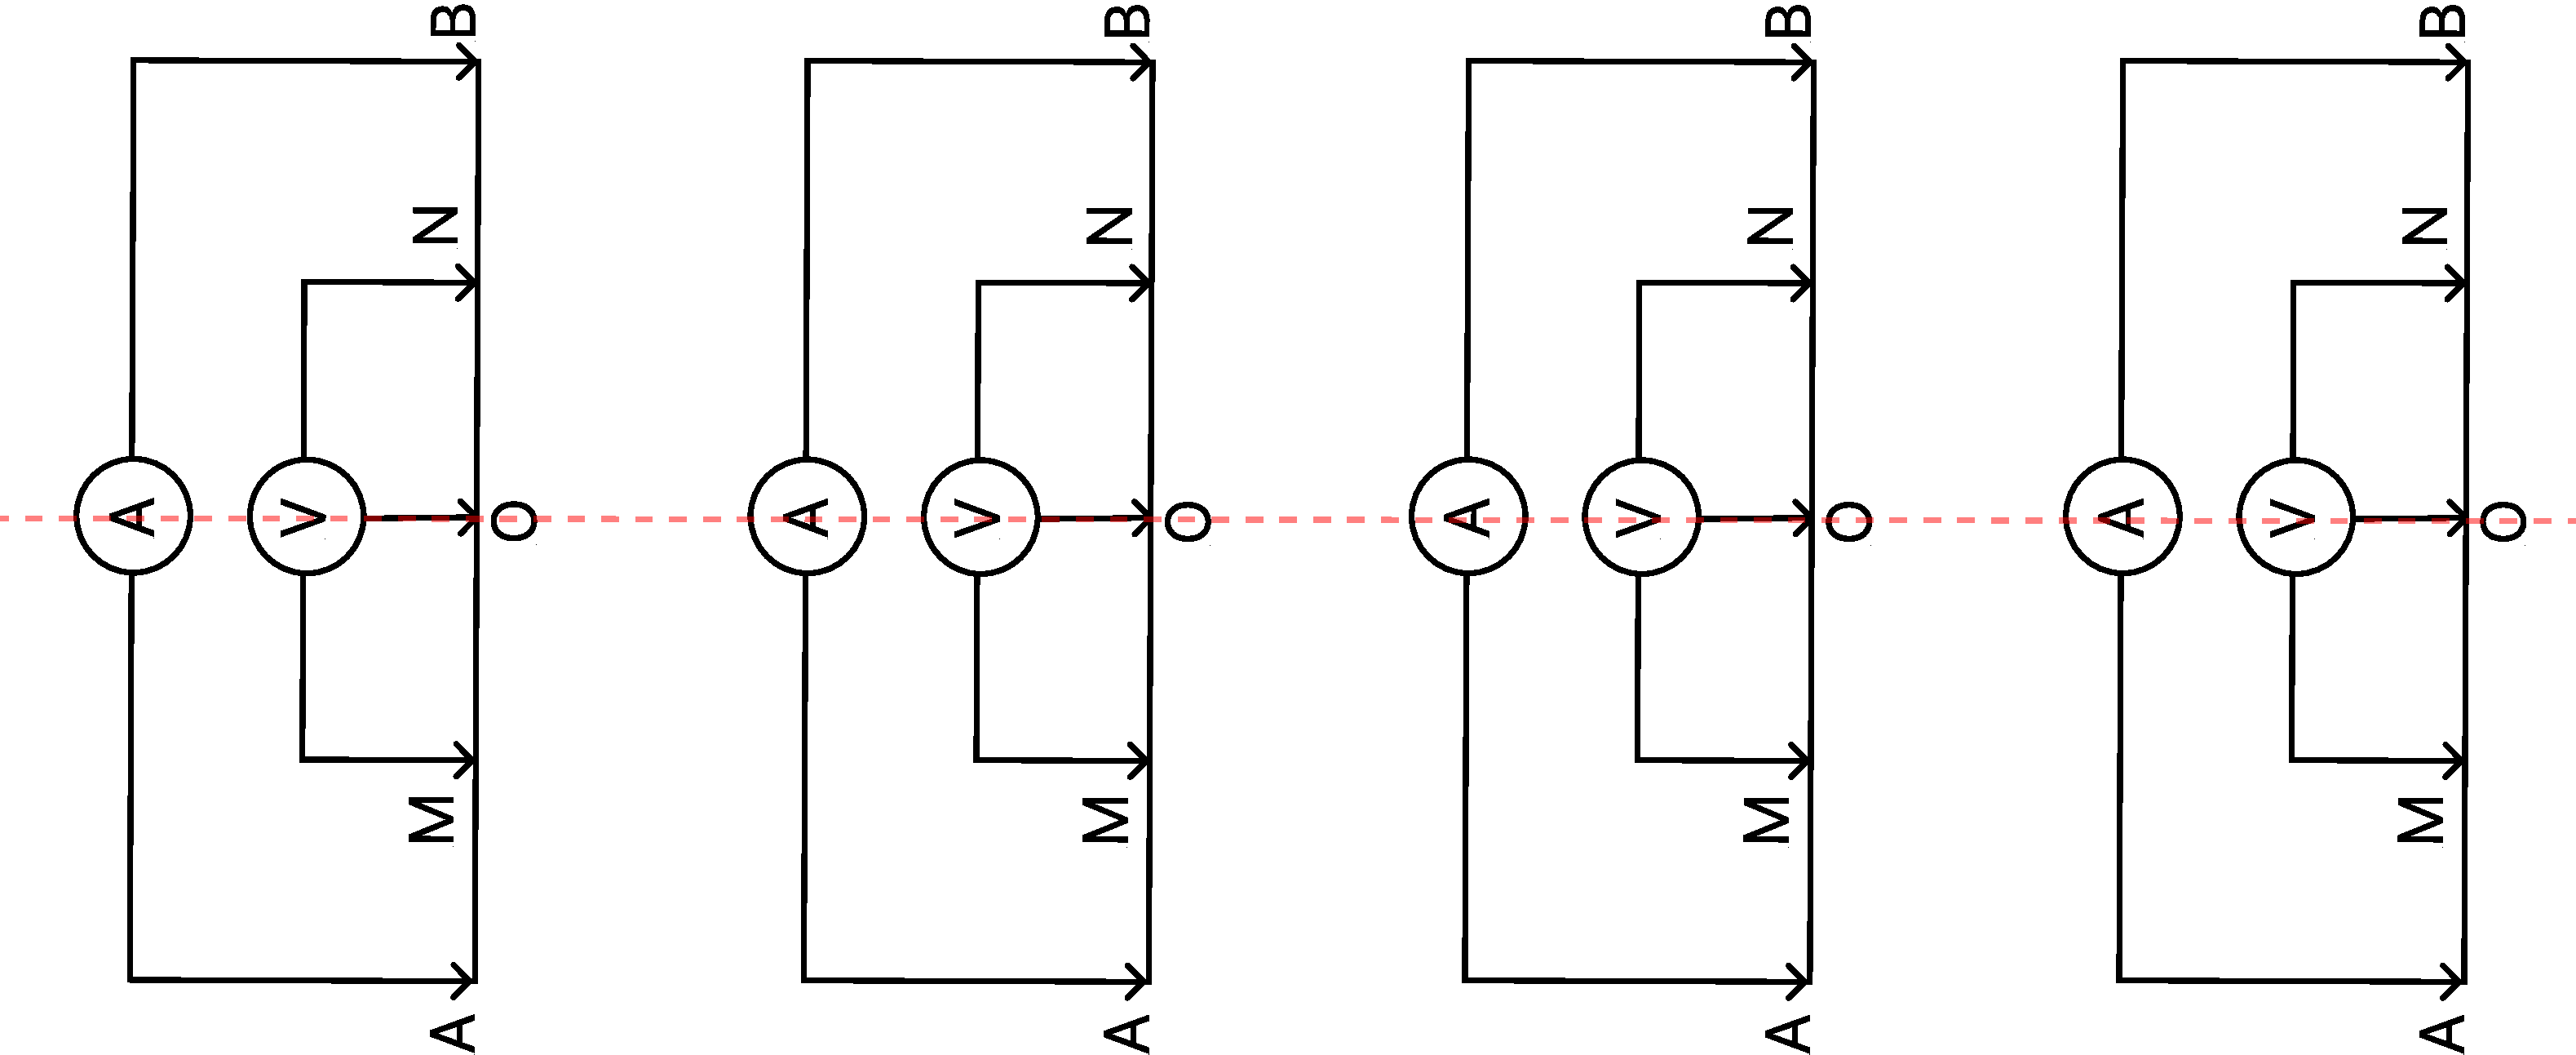
\includegraphics[width=0.75\textwidth]{gh19.pdf}
        \caption{Sondeo Horizontal}
        \label{gh19}
    \end{figure}
    \item \textbf{Vertical:} Recibe el nombre de SEV y se define como una serie de determinaciones de resistividad aparente, efectuadas con el mismo tipo de dispositivo y separación creciente de los electrodos de emisión y de recepción, permaneciendo fijos el azimut (dirección) y el centro del dispositivo. Dando como resultado información geoeléctrica del subsuelo de un mismo sitio en la vertical.
\end{enumerate}
\subsubsection{Clasificación de los SEVS}
De acuerdo a la abertura total de los electrodos de corriente, los SEV se clasifican en (Orellana, 1972)
\begin{table}[h!]
    \centering
    \begin{tabular}{@{}cc@{}}
    \toprule
    Tipo de SEV & Abertura AB (km) \\ \midrule
    Cortos      & \textless{}0.2   \\
    Normales    & 0.2-3            \\
    Largos      & \textgreater{}3  \\ \bottomrule
    \end{tabular}
    \caption{Clasificación de los SEVS}
    \label{tabgh7}
\end{table}
Los SEV que interesan en investigaciones hidrogeológicas son normales, los cortos se utilizan en la ingeniería civil y arqueología, los largos en las investigaciones petroleras.
\subsubsection{Profundidad del SEV}
En medios homogéneos, al aumentar la separación AB aumenta la profundidad en la misma proporción. Durante muchas años esto condujo a suposiciones erróneas en las que se consideraba a la profundidad del SEB como un porcentaje de la abertura AB (Normalmente se consideraba a la profundidad como un 25\% de AB)

El motivo de la interpretación errónea sobre la profundidad alcanzada por el SEV, se debe a que el suelo es un medio heterogéneo y estratificas, por lo que las reglas empíricas establecidas carecen de sentido. Incluso puede ser que la penetración de un SEV no aumente al incrementar la abertura AB, a partir de un cierto valor de ésta, ello sucederá cuando exista una capa aislante o altamente conductora a una profundidad determinada alcanzada por el SEV. En este caso, la corriente no podrá pasar por debajo de dicha capa y, por lo tanto, la profundidad alcanzada por el SEV no podrá ser mayor a la profundidad de localización de la capa mencionada.
\subsubsection{Punto de atribución del SEV}
Es el punto del terreno a cuya verticalidad deben atribuirse los resultados obtenidos por el SEV. Por razones de simetría se toma como punto de atribución de un SEV al centro 0 del dispositivo electródico. No sebe olvidarse que la medición está influenciada por un volumen de material más o menos grande.
\subsection{Corte geoeléctrico}
Para caracterizar un medio estratificado, basta indicar el espesor (E) y la resistividad ($\rho$) de cada medio parcial isótropo de índice i, numerando estos de arriba hacia abajo. Cada uno de estos medios parciales se denomina capa geoeléctrica.
\begin{figure}[h!]
\centering
  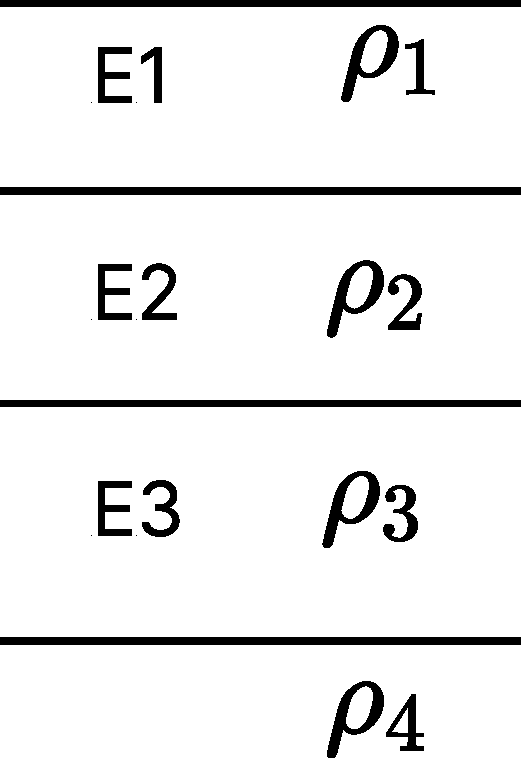
\includegraphics[width=0.25\textwidth]{gh20.pdf}
  \caption{Corte geoeléctrico}
  \label{gh20}
\end{figure}
Un corte geoeléctrico es un conjunto de capas geoeléctricas sucesivas. Para caracterizar un corte geoeléctrico de n capas, se requiere conocer n resistividades y n-1 espesores. La última capa tiene un espesor desconocido. En total se requieren 2n-1 parámetros.

Los cortes geoeléctricos se clasifican según el número de capas del mismo. Los cortes con igual número de capas se subdividen las resistividades de las mismas.
\subsubsection{Clasificación}
\begin{enumerate}
    \item \textbf{Cortes de dos capas:} Existen dos tipos y se caracterizan de la siguiente manera \begin{enumerate}
        \item $\rho_1<\rho_2$
        \item $\rho_1>\rho_2$
    \end{enumerate}
    \item \textbf{Cortes de tres capas:} Se definen cuatro tipos de cortes de tres capas. Las letras que los simbolizan son H,K,Q,A correspondientes a la figura \ref{fig21-24}: 
    \begin{figure}[h!]
        \centering
        \begin{subfigure}[b]{0.4\linewidth}
            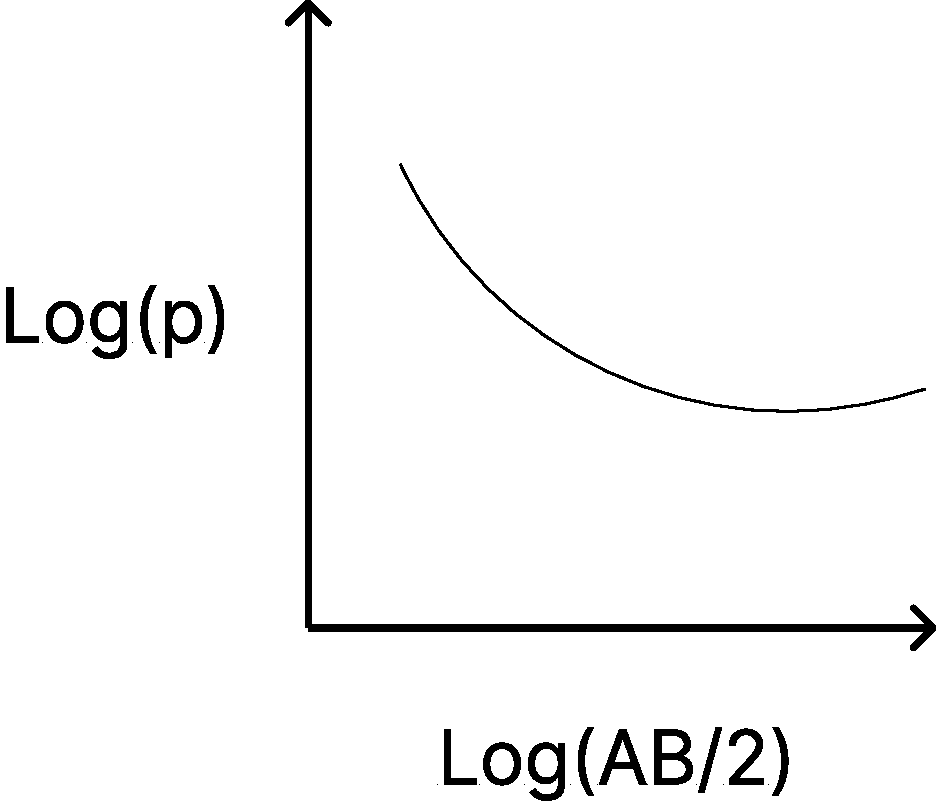
\includegraphics[width=\linewidth]{gh21.pdf}
            \caption{Tipo H}
            \label{gh21}
        \end{subfigure}
        \begin{subfigure}[b]{0.4\linewidth}
            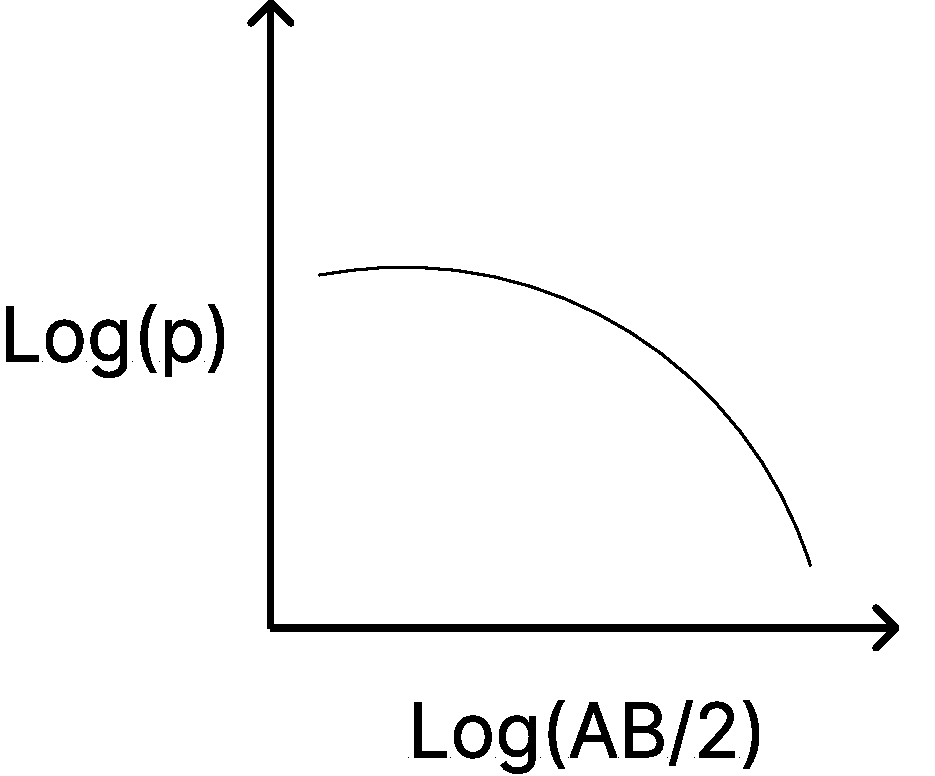
\includegraphics[width=\linewidth]{gh22.pdf}
            \caption{Tipo K}
            \label{gh22}
        \end{subfigure}
        \begin{subfigure}[b]{0.4\linewidth}
            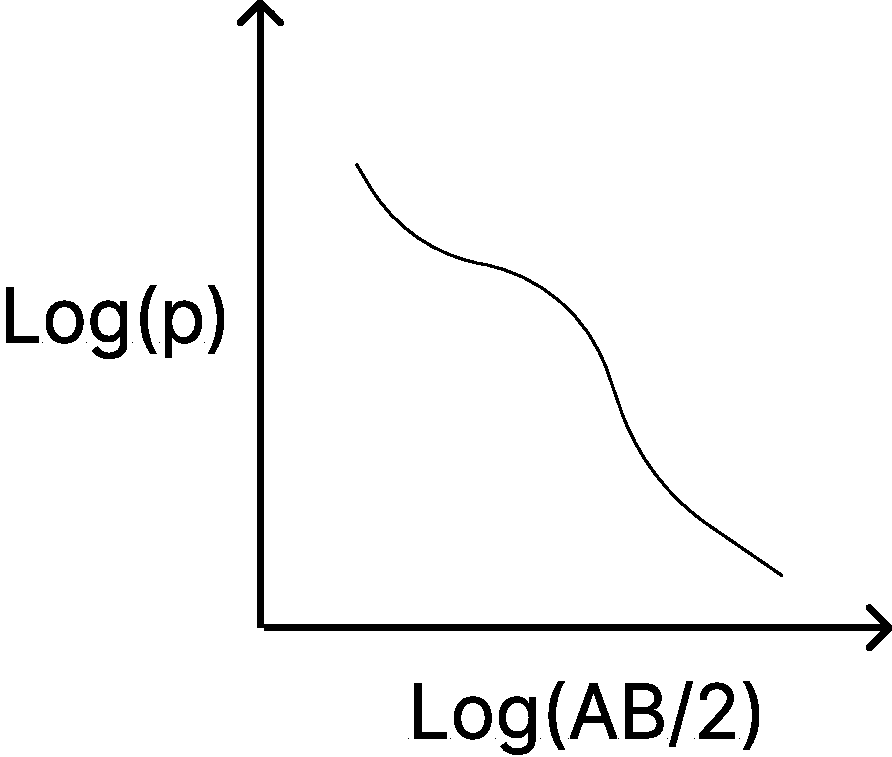
\includegraphics[width=\linewidth]{gh23.pdf}
            \caption{Tipo Q}
            \label{gh23}
        \end{subfigure}
        \begin{subfigure}[b]{0.4\linewidth}
            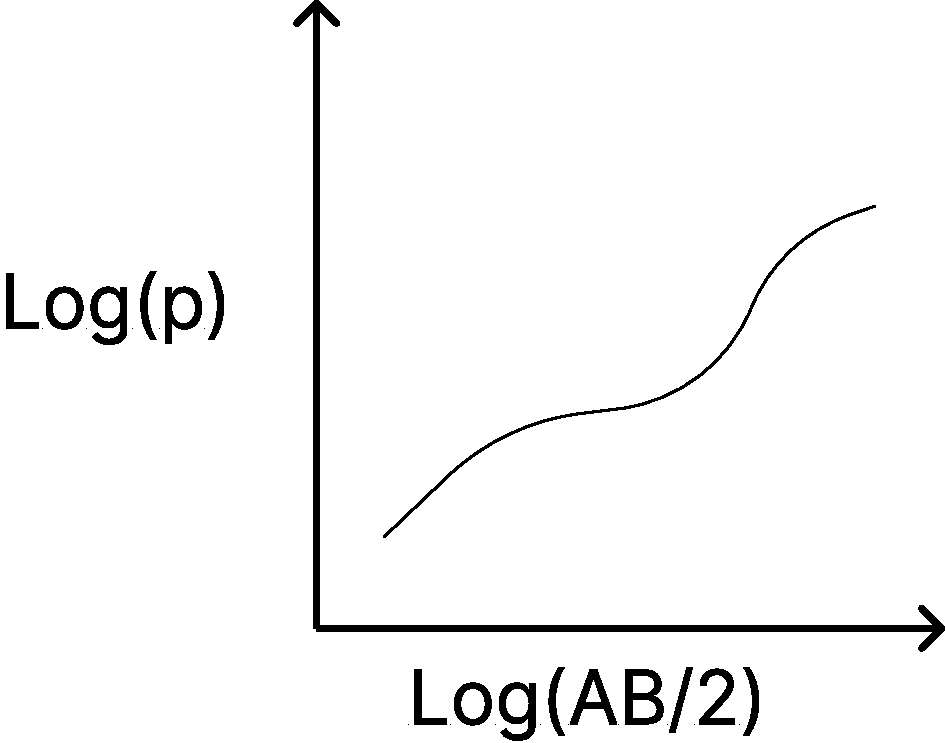
\includegraphics[width=\linewidth]{gh24.pdf}
            \caption{Tipo A}
            \label{gh24}
        \end{subfigure}
        \caption{Cortes de tres capas}
        \label{fig21-24}
    \end{figure} 
\end{enumerate}

\subsubsection{Cortes de cuatro capas}
Los cortes de cuatro capas se distribuyen en ocho grupos que se designan como combinación de las anteriores. Para ello, se consideran las tres primeras capas y se les asigna la letra corresponde de la lista anterior. Luego se hace lo mismo con las tres últimas capas. Por ejemplo el HJ corresponde a la combinación siguiente:
% TODO: Ver que show
% \begin{figure}[h!]
% \centering
%   \includegraphics[width=0.5\textwidth]{gh25.pdf}
%   \caption{Cuatro capas}
%   \label{gh25}
% \end{figure}
Así, solo son posibles los tipos HK,HA,KH, KQ, QQ, QH, AK, y AA.

\subsubsection{Cortes de cinco capas}
Se consideran en primer lugar las tres primeras  se les asigna la letra correspondiente, luego se hace lo mismo con la segunda, tercera y cuarta; después con la tercera, cuarta y quinta, y así sucesivamente hasta terminar con el total de las capas (figura \ref{gh26}).
\begin{figure}[h!]
\centering
  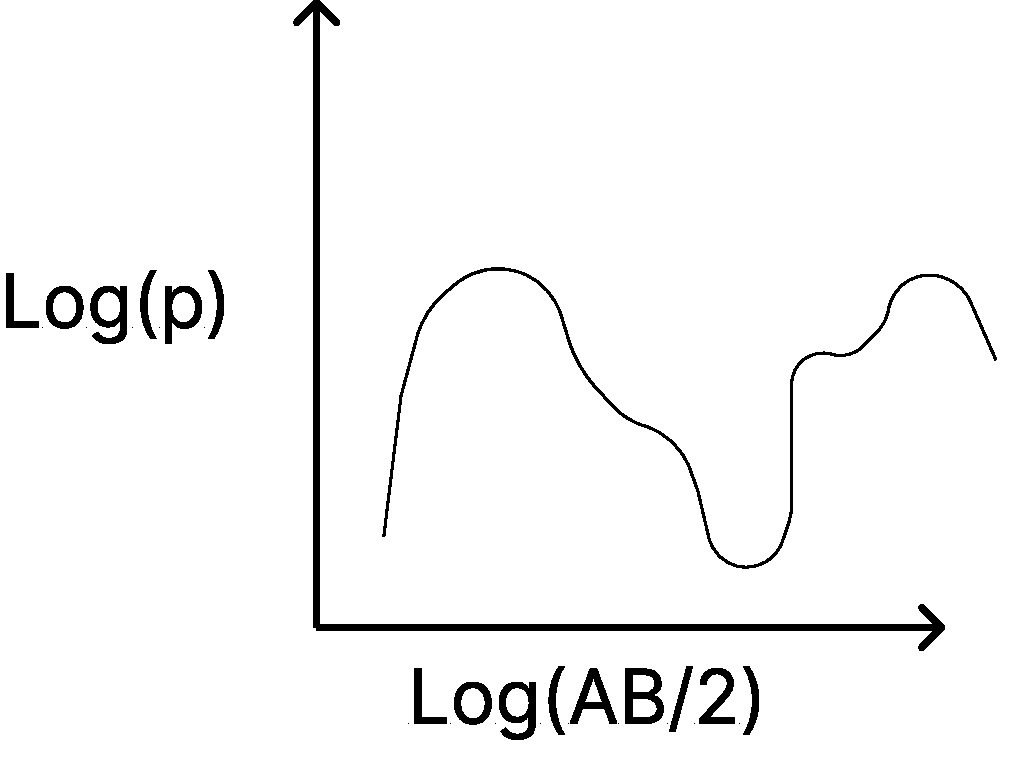
\includegraphics[width=0.5\textwidth]{gh26.pdf}
  \caption{Nueve capas: KQHAKHK}
  \label{gh26}
\end{figure}
% Qué es un traslape: Se dan en el schlumberger abertura de potencial para unir los trazos de curva, se ejecuta el sev

Método de interpretación gráfico:
\begin{itemize}
    \item Sin reducción Catálogo de curvas ya interpretadas con datos de campos, y se busca con cuál curva se ajusta en el catálogo
    \item Con reducción: Se interpreta por pares de curvas. Tiene ventaja que son baratos, pero no tiene forma de cuantificar el error y son menos precisos.
\end{itemize}
Los métodos numéricos son programas de computo excesivamente caros

\subsection{Perforación de pozos profundos para agua}
El objetivo  principal de la perforación exploratoria es el de obtener los datos necesarios para el diseño del pozo, mediante:
\begin{enumerate}
    \item Reporte diario de perforación
    \item Corte litológico
    \item Muestreo y análisis de roca y agua
    \item Registro eléctrico
    \item Análisis granulométrico
\end{enumerate}
\textbf{Métodos de perforación:}
\begin{itemize}
    \item Percusión: Dejar caer una herramienta con mucho peso para romper las capas del suelo
    \item Rotatorio: Es un taladro que excava con mucha eficiencia 
    \item Rotopercusión: Combina la acción de percusión y rotatorio
\end{itemize}
\subsubsection{Método de percusión}
Es adecuado para formaciones rocosas o estables y suaves; no coherentes o granulares.

Las tijeras sirven para no rebotar el impacto al resto del barreno.
La broca de serpentín, es la que se deja caer en materiales finos de arcilla para licuar el suelo y dejarlos suspendidos.

Luego para extraer los restos de piedras, se usa una cuchara 

% Material tipo 1 son porosas, mientras que el tipo 3 son las rocas sanas y la tipo 2

% No se necesita un proceso de diseño si se cuenta con un conocimiento geológico del lugar

Ventajas del método de perforación por percusión:
\begin{itemize}
    \item Alto rendimiento en material duro
    \item Muestreo confiable de las formaciones atravesadas se tomarían muestras con mínimo 1 a 2 metros hasta 6 metros consignado en el contrato de perforación
    \item Registro independiente de niveles de agua en las formaciones atravesadas
    \item La perforación no requiere de grandes cantidades de agua
    \item Los equipos son más fáciles de operara 
\end{itemize}
Desventajas:
\begin{itemize}
    \item Se pierde el ademe si el sitio no resulta favorable (si es que este se ademó)
    \item El rendimiento decrece conforme aumenta la profundidad del pozo
    \item No hay flexibilidad para cambiar el diámetro de perforación, cuando se adema
    \item Verticalidad y diámetro relativo a las formaciones geológicas
    \item Baja velocidad de penetración en acarreos y formaciones no consolidadas
    \item No permite hacer diseño del pozo
\end{itemize}
\subsubsection{Método rotatorio}
Se emplea en la mayoría de formaciones, menos en rocas carstificadas o con fracturamiento
\begin{figure}[h!]
\centering
  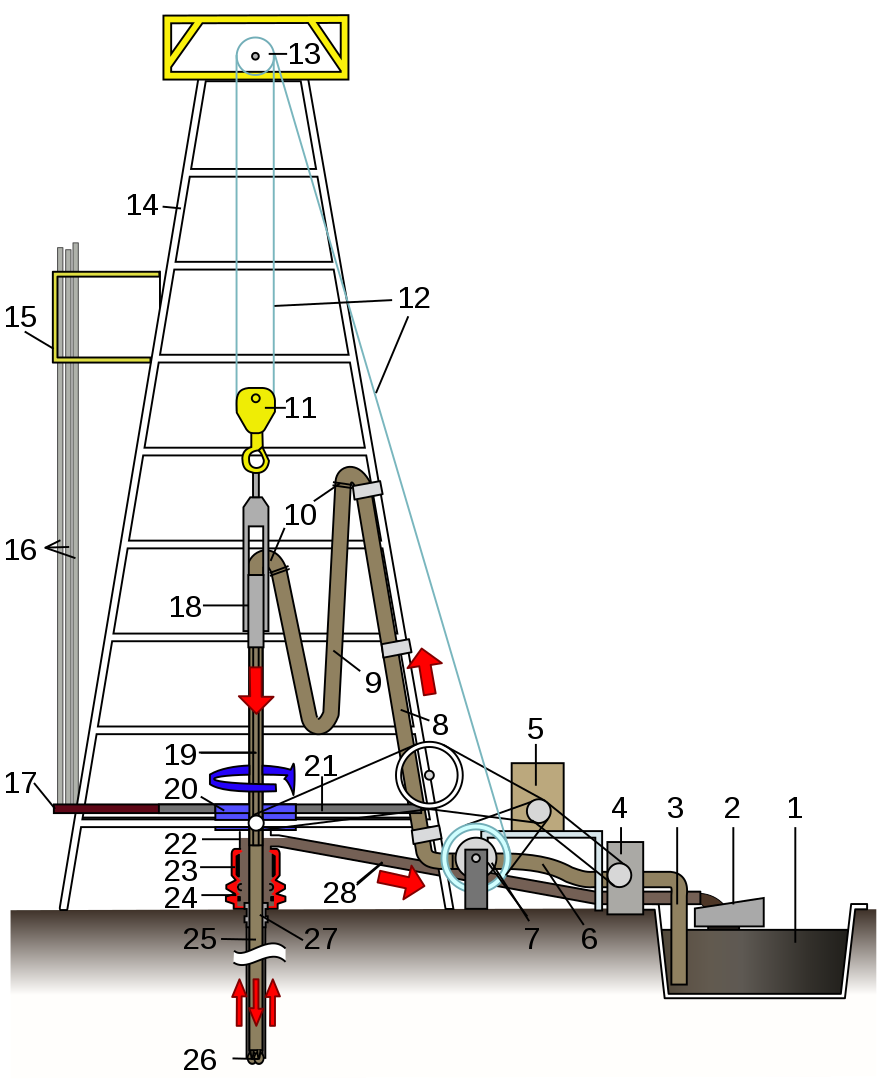
\includegraphics[width=0.75\textwidth]{gh27.png}
  \caption{Método rotatorio}
  \label{gh27}
\end{figure}
1. Es el \textbf{tanque de lodo}, y es el depósito donde se almacena el fluido de perforación denominado también lodo de perforación.

2. Es el \textbf{agitador} en el tanque de lodo, el cual es el encargado de estar agitando los componentes que componen el fluido de perforación para que este mantenga sus propiedades según dictamine el programa de perforación.

3. \textbf{Línea de succión}, termina siendo el medio de comunicación entre el tanque de lodo y la bomba de succión que es a la final el componente que succiona el fluido de perforación desde los tanques hasta el fondo del pozo.

6 y 8. \textbf{Manguera vibratoria y tubo vertical}, la razón por la que combino estos dos componentes es por de igual manera el fluido de perforación circula por esta dos partes.

9. \textbf{Manguera Kelly}, el punto 9 es la continuidad de la misma manguera por donde circula el fluido de perforación, con la excepción de que se denomina manguera Kelly porque queda por debajo del cuello de ganso.

10. \textbf{Cuello de ganso}, es la parte superior de los extremos de la manguera de circulación que parece como un codo, quizás muchos se pregunten porque tienen estos nombres tan raros, recuerden que gran parte del conocimiento heredado por parte de las industrias norteamericana era de un vocablo técnico que contemplaba estos nombres que por hoy es muy común encontrar en la industria petrolera, sobre todo en perforación.

18. \textbf{Unión giratoria}, es la encargada de hacer girar la sarta de perforación, en la perforación de pozos se puede conseguir también con el nombre de junta Kelly.

20. \textbf{Mesa rotatoria}, gira porque la unión giratoria la hace girar, al girar la mesa rotatoria gira la sarta de perforación.

25. \textbf{Sarta de perforación}, la conforma el ensamblaje de fondo (BHA) que está conformado por tubos pesados como collares de perforación (drill collars) y tubería pesada de transición (heavy weight), junto con el bha se ensambla la tubería de perforación que es la que finalmente le da profundidad al pozo.

Las mechas de perforación se conectan a la primera barra de perforación, por lo que se pudiera decir que la mecha de perforación también pertenece al ensamblaje de fondo (BHA), entre las mechas de perforación existen mechas PDC, de diamante, policristalinas y tricónicas.


% carburo de tungsteno

% El sedaso evita que el pozo se asolve pero pueda permitir el paso de agua con eficiencia, la forma de sus orificios son hidrodinámicas para que no pierda carga

Ventajas del método rotatorio
\begin{itemize}
    \item Mayor velocidad de avance
    \item No es necesario utilizar ademe para sostener las paredes de la formación al estar perforado
    \item Gran flexibilidad para variar el diámetro de la perforación
    \item El ademe no se pierde si el pozo resulta fallido (ya que no es necesario)
    \item Alta velocidad de penetración en acarreos
    \item Alto rendimiento a profundidad
\end{itemize}
Desventajas
\begin{itemize}
    \item Las pérdidas de lodo reducen notablemente la permeabilidad de las formaciones acuíferas
    \item Muestreo de materiales no es muy representativo
    \item No es posible registrar independientemente los niveles estáticos, ni la calidad del agua de las formaciones atravesadas.
    \item No apropiado para rocas fracturadas o con conductos de disolución, donde la pérdida total de lodo impide continuar la perforación
    \item Requiere grandes cantidades e agua y personal más especializado
    \item Mantenimiento costoso el equipo
\end{itemize}
\subsubsection{Método de rotación-percusión}
\begin{figure}[h!]
\centering
  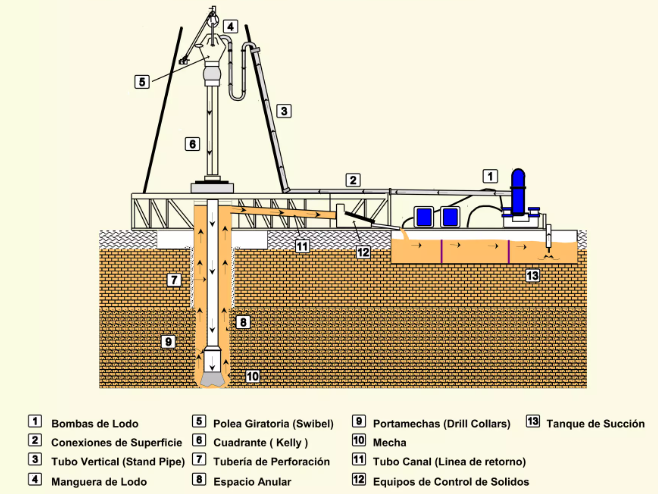
\includegraphics[width=1\textwidth]{gh28.png}
  \caption{Método de rotación-percusión}
  \label{gh28}
\end{figure}
Ventajas:
\begin{itemize}
    \item Gran velocidad de perforación
    \item Gran verticalidad del pozo
    \item Escasa contaminación del acuífero por el tipo de fluido utilizado
\end{itemize}
Desventajas:
\begin{itemize}
    \item Es bastante caro
    \item Requiere personal muy especializado
\end{itemize}
\subsubsection{Etapas posteriores a la perforación exploratoria}
\begin{itemize}
    \item Diseño del pozo
    \item Terminación 
    \item Aforo del pozo
    \item Diseño del equipo de bombeo
    \item Instalación del equipo
    \item Operación
\end{itemize}
\section{Diseño de pozo profundo para agua}
\subsection{Procedimiento de diseño}
\subsubsection{Cámara de bombeo}
\begin{figure}[h!]
\centering
  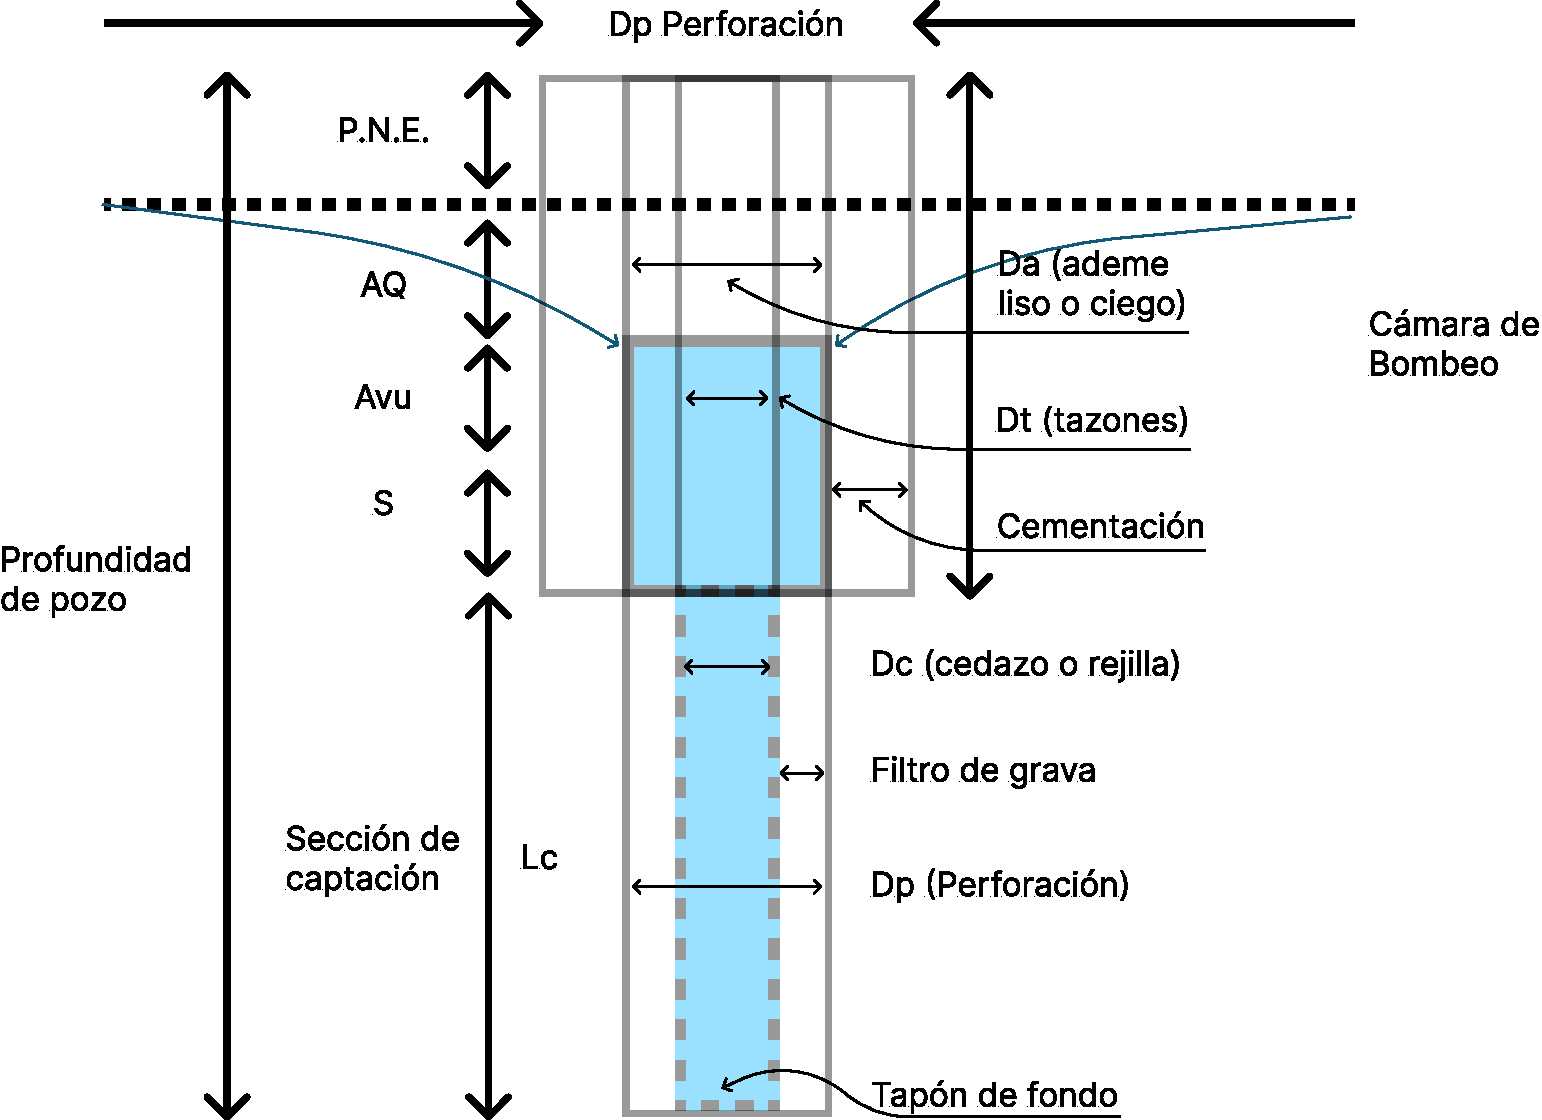
\includegraphics[width=0.75\textwidth]{gh30.pdf}
  \caption{Cámara de bombeo}
  \label{gh30}
\end{figure}
La longitud de la cámara de bombeo ($L_{cb}$) se obtiene en función de los siguientes parámetros:
\begin{equation}
    L_{cb} = 1.1\left(P.N.E + A_Q + A_{vu} + S\right)
\end{equation}
Esto en tramos de $20^{\prime}$ (Longitud comercial)
\begin{notation}
    \begin{itemize}
        \item $PNE=$ Profundidad del Nivel Estático
        \item $AVu=$ Abatimiento esperado del novel estático durante la vida útil del pozo, se consideran 25 años mínimo ($A_R$ en metros de abatimiento anual del N.E. por 25-30 años de vida útil).
        \item $A_Q$ Abatimiento del nivel del agua en el interior del pozo provocado por el caudal de extracción considerado ($A_Q$) 
        \begin{equation}
            A_Q = \frac{Q_{\text{diseño}}}{Q_{especifico}}
        \end{equation}
        \item $S=$ Sumergencia mínima de la bomba para su funcionamiento óptimo (Se considera un metro de sumergencia de la bomba por cada 7.5lps de extracción)
    \end{itemize}
\end{notation}
\begin{equation}
    T = 1.2Q_e
\end{equation}
El diámetro de adame ciego ($D_a$) y diámetro de perforación ($D_p$)

Se obtiene a partir del diámetro de tazones:
\begin{equation}
    D_t = \sqrt{Q}
\end{equation}
(Q de diseño en lps. $D_t$  se lleva a par superior en pulgadas)
\begin{equation}
    D_a = D_t + 2\left(2^{\prime\prime}\, a\, 3^{\prime\prime}\right)
\end{equation}
($2^{\prime\prime}$ a $3^{\prime\prime}$ de holgura de cada lado del tazón, por economía se usa $2^{\prime\prime}$)
\begin{example}
    Ejercicio de diseño de pozo, en campo experimental para $Q=34lps$
    
    \textit{ Sol. }

    \begin{align*}
        &L_{cb} = 1.1\left(P.N.E + A_Q + A_{vu} + S\right)\\
        &L_{cb} = 1.1\left( 97.5m + \frac{34 lps}{5 \frac{lps}{s}} + 1.6\frac{m}{año} \left(25\, \text{años}\right) + \frac{34 lps}{7.5 \frac{lps}{m}}    \right)\\
        &L_{cb} = 1.1 (1.48.8m) = 163.7m = 28.86 \text{ Tramos de } 20^{\prime}\\
        &L_{cb} = 27 \cdot 20 \cdot 0.3048 = 164.6m
    \end{align*}
\end{example}
Diámetro de perforación en la cámara de bombeo ($D_p$)
\begin{equation}
    D_p = D_a + 2\left(3^{\prime\prime}\right)
\end{equation}
($3^{\prime\prime}$ de espesor de sección anular en donde va cementación en toda la longitud de la cámara de bombeo o mínimo 30m de ella, para incrementar la resistencia mecánica del ademe y por protección sanitaria).

Diámetro de ademe ciego ($D_a$)

Se obtiene a partir del diámetro de tazones:
\begin{equation}
    D_t = \sqrt{34} = 5.83\implies 6^{\prime\prime}
\end{equation}
(Q de diseño en lps. Dt se lleva a par superior en pulgadas):
\begin{equation}
    D_a = D_t + 2(\text{2 a 3})= 6+2(2^{\prime\prime}) = 10^{\prime\prime}
\end{equation}
($2^{\prime\prime}$ a $3^{\prime\prime}$ de holgura de cada lado del tazón, por economía $2^{\prime\prime}$)
Diámetro de perforación en la cámara de bombeo ($D_p$):
\begin{equation}
    D_p = D_a + 2(3) = 10 + 2(3) = 16^{\prime\prime}
\end{equation}
($3^{\prime\prime}$ de espesor de sección anular en donde va cementación en toda la longitud de la cámara de bombeo o mínimo 39 m de ella, para incrementar la resistencia mecánica del ademe y por protección sanitaria)\dots
\begin{table}[h!]
    \centering
    \begin{tabular}{@{}ccc@{}}
    \toprule
    \begin{tabular}[c]{@{}c@{}}Diámetro\\ (pulgadas)\end{tabular} &
      \begin{tabular}[c]{@{}c@{}}Espesor\\ (pulgadas)\end{tabular} &
      \begin{tabular}[c]{@{}c@{}}Prof. Máxima\\ recomendable (m)\end{tabular} \\ \midrule
    10 & 3/16 & 130 \\
    12 & 3/16 & 90  \\
    14 & 3/16 & 75  \\
    16 & 3/16 & 55  \\
    10 & 1/4  & 235 \\
    12 & 1/4  & 165 \\
    14 & 1/4  & 135 \\
    16 & 1/4  & 105 \\
    18 & 1/4  & 80  \\
    20 & 1/4  & 65  \\
    10 & 5/16 & 370 \\
    12 & 5/16 & 260 \\
    14 & 5/16 & 210 \\
    16 & 5/16 & 160 \\
    18 & 5-16 & 125 \\
    20 & 5-16 & 100 \\
    16 & 3/8  & 235 \\
    18 & 3/8  & 185 \\
    20 & 3/8  & 150 \\ \bottomrule
    \end{tabular}
    \caption{Espesor del ademe ciego (e)}
    \label{tabgh8}
\end{table}
\begin{itemize}
    \item Profundidades máximas recomendables para diferentes espesores y diámetros de tubería de acero (Recomendación API con un f.s. de 30\%)
    \item Espesor mínimo recomendado $1/4^{\prime\prime}$ en acero
\end{itemize}

\subsubsection{Sección de captación}
Depende del espesor y estratificación del acuífero  y del gasto. En acuíferos confinados y semiconfinados se recomineda captar de preferencia el total del estrato aportador, o mínomo el 70\% de este. En acuíferos libres de espesores considerables se recomienda captar minimo $b/3$ para minimizar problemas de penetración parcial

Abertura de rejilla. cuando el pozo requiere de un filtro de grava, las aberturas de rejilla se determinan en función de la granulometría de estre filtro, la que a su vez depende de la granulometría del acuífero. Para la determinación tanto de la granulometría, como de y abertura de la rejilla, se usa el método de Johnson.
\subsubsection{Diseño de filtro de grava y abertura de rejilla por el método Jhonson}

Dibujar la curva granulométrica del material acuífero más fino a captar
\begin{figure}[h!]
\centering
  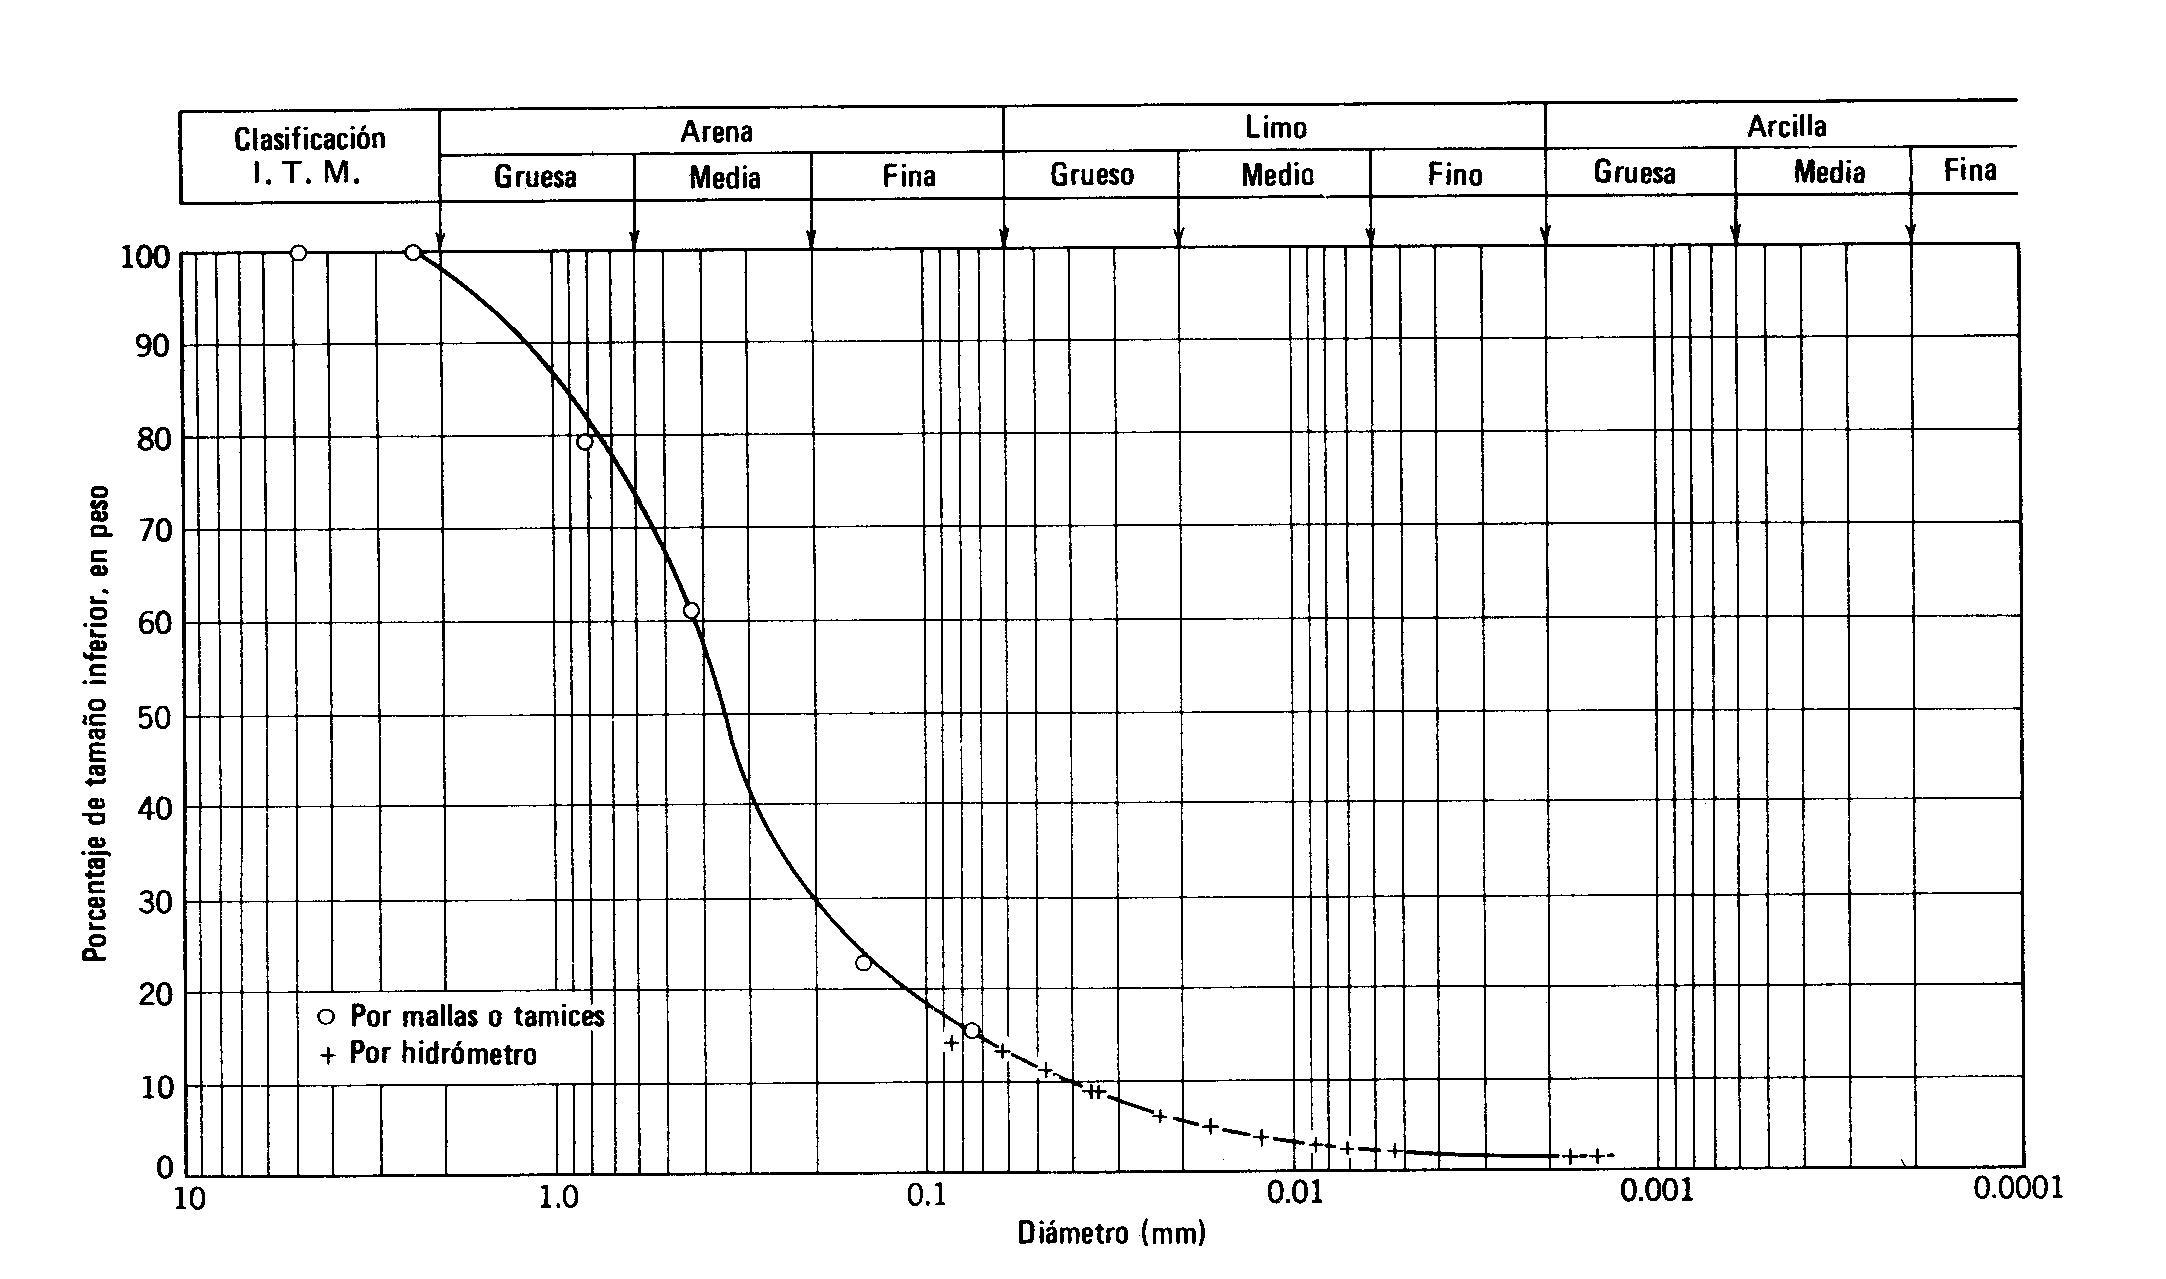
\includegraphics[width=0.9\textwidth]{gh29.jpg}
  \caption{Curva granulométrica}
  \label{gh29}
\end{figure}

El $D_{70}$ de la curva se multiplica por un factor entre 4 y 6 (5 valor medio), y este será el $D_{70}$ de la curva del filtro de grava.

Se obtiene una curva del filtro suave y continua que pase por el $D_{70}$ y que tenga un coeficiente de uniformidad $C_u\leq 2.5$ por tanteos.
\begin{equation}
    Cu = \frac{D_{40}}{D_{90}}
\end{equation}

Se seleccionan mínimo cuatro puntos distribuidos en la curva, los cuales serán la especificación del filtro de grava y se establece un rango permisible de $\pm 8\%$

Se selecciona el R de la curva como la abertura de rejilla, capaz de retener mínimo el 90\% del material del filtro.
\begin{table}[h!]
    \centering
    \begin{tabular}{@{}ccc@{}}
    \toprule
    Abertura de rejilla (mm) & Filtro de grava ($^{\prime\prime}$) & Factor de obturamiento (F.O.) \\ \midrule
    1 & 1/8-1/4 & 2   \\
    2 & 1/4-1/2 & 1.5 \\
    3 & 1/2-3/4 & 1.25   \\
    3-7 & >3/4  & 1.1   \\ \bottomrule
    \end{tabular}
    \caption{Recomendaciones prácticas de constructores de pozos}
    \label{tabgh9}
\end{table}
Longitud de cedazo o rejilla ($L_c$). En el cálculo de longitud y diámetro de cedazo se emplea un catálogo de rejillas, el cual puede ser tipo canastilla (puentecillo), concha o ranurado.
\begin{table}[h!]
    \centering
    \begin{tabular}{@{}ccccc@{}}
    \toprule
    \multirow{2}{*}{Diámetro y espesor (pulg.)} &
      \multirow{2}{*}{Peso por metro lineal (kg)} &
      \multicolumn{3}{c}{Abertura de la ranura (mm)} \\ \cmidrule(l){3-5} 
     &
       &
      1 &
      2 &
      3 \\ \midrule
    \begin{tabular}[c]{@{}c@{}}83/16\\   1/4\\  103/16\\   1/4\\  12 1/4\\   5/16\\  14 1/4\\   5/16\\  16 1/4\\   5/16\\  18 1/4\\   5/16\\  20 1/4\\   5/16\\  22 1/4\\   5/16\\  24 1/4\\   5/16\end{tabular} &
      \begin{tabular}[c]{@{}c@{}}25.2\\  34.3\\  31.9\\  42.8\\  50.7\\  61.7\\  55.7\\  69.8\\  64.3\\  80.9\\  72.3\\  91.5\\  80.6\\  101.9\\  88.1\\  110.8\\  96.5\\  120.9\end{tabular} &
      \begin{tabular}[c]{@{}c@{}}316\\  316\\  391\\  391\\  474\\  474\\  515\\  515\\  574\\  574\\  665\\  665\\  740\\  740\\  823\\  823\\  898\\  898\end{tabular} &
      \begin{tabular}[c]{@{}c@{}}608\\  608\\  752\\  752\\  912\\  912\\  992\\  992\\  1104\\  1104\\  1280\\  1280\\  1424\\  1424\\  1584\\  1584\\  1728\\  1728\end{tabular} &
      \begin{tabular}[c]{@{}c@{}}985\\  985\\  1218\\  1218\\  1477\\  1477\\  1607\\  1607\\  1788\\  1788\\  2073\\  2073\\  2306\\  2306\\  2566\\  2566\\  2799\\  2799\end{tabular} \\\midrule
    \end{tabular}
    \caption{Área de filtración en $cm^2$ ($A_u$) por metro lineal de rejilla tipo canastilla vertical, de acero.}
    \label{tabgh10}
    \end{table}

El área efectiva ($A_e$) de paso por la rejilla:
\begin{equation}
    A_e =\left(1 - obt \right)A_u \cdot  L_c
\end{equation}
Donde $A_u$ es el área abierta o de filtración para un diámetro, abertura y tipo de rejilla, en $m^2/m$. $L_c$ es longitud de cedazo en m.
\begin{equation}
    L_c = \left(\frac{1}{1 - obt}\right) \frac{A_e}{A_u}
\end{equation}
Al sustituir la ecuación de gasto $Q=AV$ y $F_o= 1/(1-obt)$, se obtiene:
\begin{equation}
    L_c = F_o \frac{Q}{A_u V_p}
\end{equation}
Donde Q es gasto de diseño y $V_p$ es velocidad permisible, se acepta que $V_p=3-5cm/s$

El diámetro del cedazo deberá ser menor o a lo mucho igual al ademe ciego.

El espesor de la rejilla será $1/16^{\prime\prime}$ mayor que el espesor del ademe, su $D_c=D_a$.

El diámetro de perforación en la sección de captación se recomienda de $4^{\prime\prime}$ a $6^{\prime\prime}$ mayor que el diámetro del cedazo, para alojar el filtro de grava.

\begin{problem}[Sin restricción de b]
    Para una abertura de rejilla de 2mm tipo canastilla vertical y un diámetro de cedazo igual al del ademe ciego $Dc=Sa=10^{\prime\prime}$, el área unitaria, $A_u$ es $752 cm^2/m$

    El factor de obturamiento para abertura de 2mm es 1.5
    \begin{equation*}
        L_c = F_o \frac{Q}{A_uV_p}= 1.5 \frac{0.034}{0.0752(0.04)} = 16.95m\implies \frac{16.95}{6.096} = 2.78\text{ tramos de } 20^{\prime}
    \end{equation*}

    Se emplearían tres tramos de $20^{\prime}$, lo cual implicaría $L_c= 3\cdot 6.096= 18.3m$ con un espesor de $1/4^{\prime\prime}$ de rejilla en acero es suficiente. El diámetro de perforación quedaría: $D_p= D_c+6^{\prime\prime}= 16^{\prime\prime}$

    El pozo quedaría recto de una profundidad total: $P_{pozo}=L_{cb}+L_c= 164.6+18.3=183m$
\end{problem}

\begin{problem}[Acuífero confinado de $b=50m$]
    Según recomendación se captará mínimo 0.7b, es decir $L_c=0.7*50=35m$, para esta longitud se podrá emplear un $D_c=8^{\prime\prime}$, así para la abertura de rejilla de 2mm tipo canastilla vertical, el área unitaria, $A_u$ es $608cm^2/m$

El facto de obturamiento para la abertura de 2mm es 1.5

Lo que se verificará es que la $V_p$ esté en el rango de 3-5cm/s
\begin{equation*}
    \frac{35}{6.096} = 5.74\implies 6 \text{ Tramos de } 20^{\prime} \implies 36.6m\\
    V_p = Fo \frac{Q}{A_u L_c} = 1.5 \frac{0.034}{0.0608 \cdot 36.6 } = 0.023 \frac{m}{s}
\end{equation*}
Ya que no hay rejillas de menor diámetro, se eligiría esta y quedaría un poco sobrada.

Con un espesor de $1/4^{\prime\prime}$ de rejilla en acero es suficiente. El diámetro de perforación quedaría: $D_p= D_c+6^{\prime\prime} = 14^{\prime\prime}$
\end{problem}

\subsection{Terminación del pozo}
La terminación del pozo se realiza de acuerdo al diseño del mismo, y se considera la segunda etapa constructiva. Consiste en los trabajos siguientes:
\begin{enumerate}
    \item Ampliación: Se lleva a cabo mediante ampliadores o rimas, en cuyo extremo se coloca una barrena guía del mismo diámetro que la perforación exploratoria
    \item Ademado: Consiste en la colocación de la tubería en el interior del pozo. Deberá verificarse que la tubería entre libremente, quedando estrictamente prohibido hincarla a golpes. Los tramos tanto de rejilla como de ademe ciego van soldados
    \item Engravado: Consiste en la colocación del filtro de grava de río de materiales redondeado, No material triturado, ni calcáreo
    \item Cementación: Esta consiste en la colocación de lechada de cemento en el espacio anular entre el ademe ciego y la pared del pozo(min. 30m). Su objetivo es estabilizar el terreno y evitar el ingreso de agua de mala calidad. (encima de la grava va un tapón de arcilla de 2 a 3 metros de espesor).
    \item Lavado primario: Consiste en desalojar del interior del pozo y del filtro de gravas el máximo de lodo bentonítico utilizado durante la perforación
    \item Tratamiento con dispersor de arcillas: Consiste en aplicar al pozo, agentes químicos dispersores de arcillas (SC-100, Well-Aid, Serwell, Disper Al, otros) con el objeto de eliminar mediante defloculación de la arcilla, el enjarre de las paredes del pozo, en el filtro de grava en las ranuras del cedazo
    \item Limpieza y agitación mecánica del pozo: Consiste en agitar mecánicamente al pozo, mediante la acción reciprocante de un pistón de empaque de hule o cuero. Provocando una acción diámica que origina un desarrollo incipiente en el filtro de grava y formación acuífera cercana al pozo. El azolve provocado por lo anterior deberá extraerse con un acuchara apropiada
    \item Desarrollo por bombeo: Este método generalmente se aplica como la etapa final del desarrollo inicial previamente logrado en la acción anterior. Se realiza con bomba turbina vertical y motor de combustión interna a velocidades de rotación variable y por ende gastos variables (etapas), la duración de cada etapa de ser gasta que el agua salga limpia, o empiece a interrumpirse el flujo (bloqueo). Desde $Q_{min}$ Hasta $1.5 Q_{\text{diseño}}$. Incrementando la velocidad del motor (N) 100rpm en cada etapa.  
\end{enumerate}
\begin{figure}[h!]
\centering
  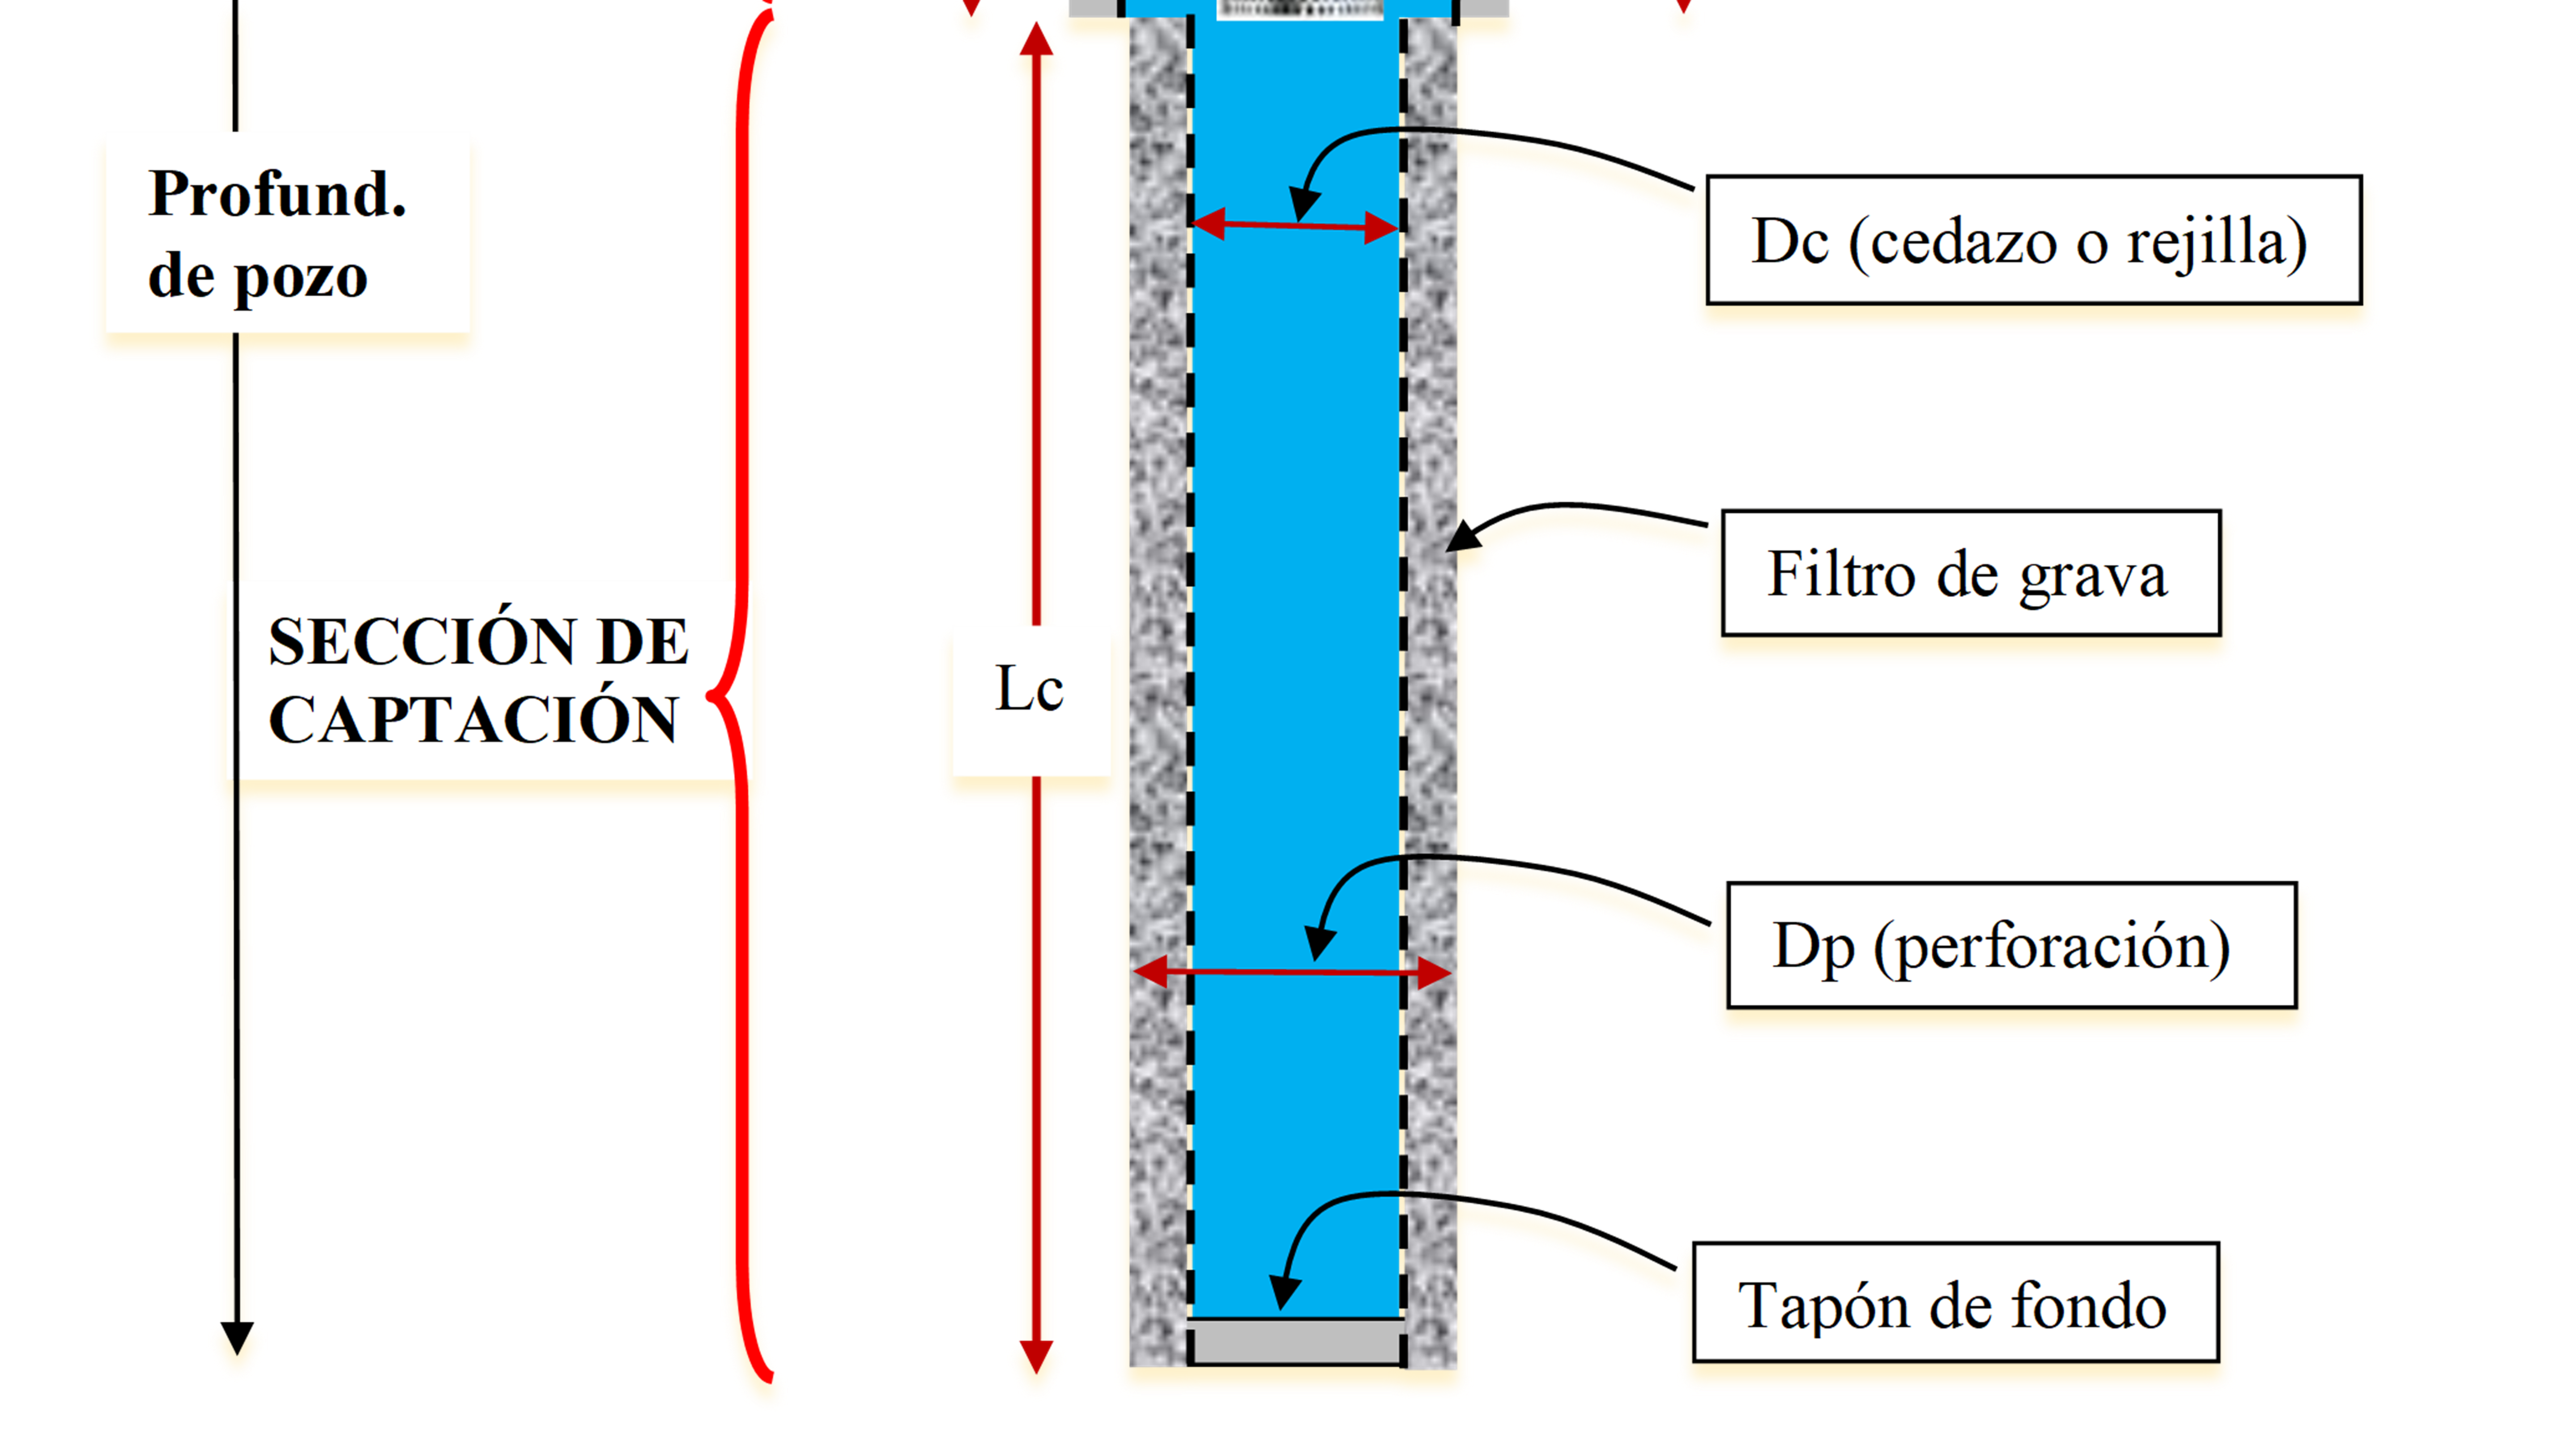
\includegraphics[width=0.75\textwidth]{gh31.png}
  \caption{Sección de captación}
  \label{gh31}
\end{figure}

% %%%%%%%%%%%%%%%%%%%%%%%%%%%%%%%%%%%%%%%%%%%%

\subsection{Aforo del pozo}
Es conocida como la \textbf{prueba de bombeo escalonada}, debe tener mínimo de 50 a 51L capacidad mínima del equipo de bombeo a gastos escalonados.

Mínimo cuatro gastos diferentes y crecientes desde un co-mínimo a un co-máximo. $Q_{min}= 1.5Q$ diseño, la duración de cada etapa es de 3-6 horas, dando un total de 12-72 horas.

% \begin{table}[h!]
%     \centering
%     \begin{tabular}{cc}
%     \hline
%     CLASE DE ESTRUCTURA & FC   \\ \hline
%     A                   & 1.00 \\
%     B                   & 0.95 \\
%     C                   & 0.90 \\ \hline
%     \end{tabular}
%     \caption{ Factor de tamaño, $F_C$}
%     \label{tabgh}
% \end{table}

Objetivos:
\begin{itemize}
    \item Determinar el gasto de explotación
    \item Determinar las componentes del abatimiento
    \item Obtener la eficiencia del pozo
    \item Conocer el caudal específico $Q_e$ (caudal entre abatimiento)
\end{itemize}
\subsubsection{interpretación de la prueba de aforo}
\begin{align}
    &a = a_f + a_p\\
    &a = BQ + CQ^2
\end{align}
\begin{figure}[h!]
\centering
  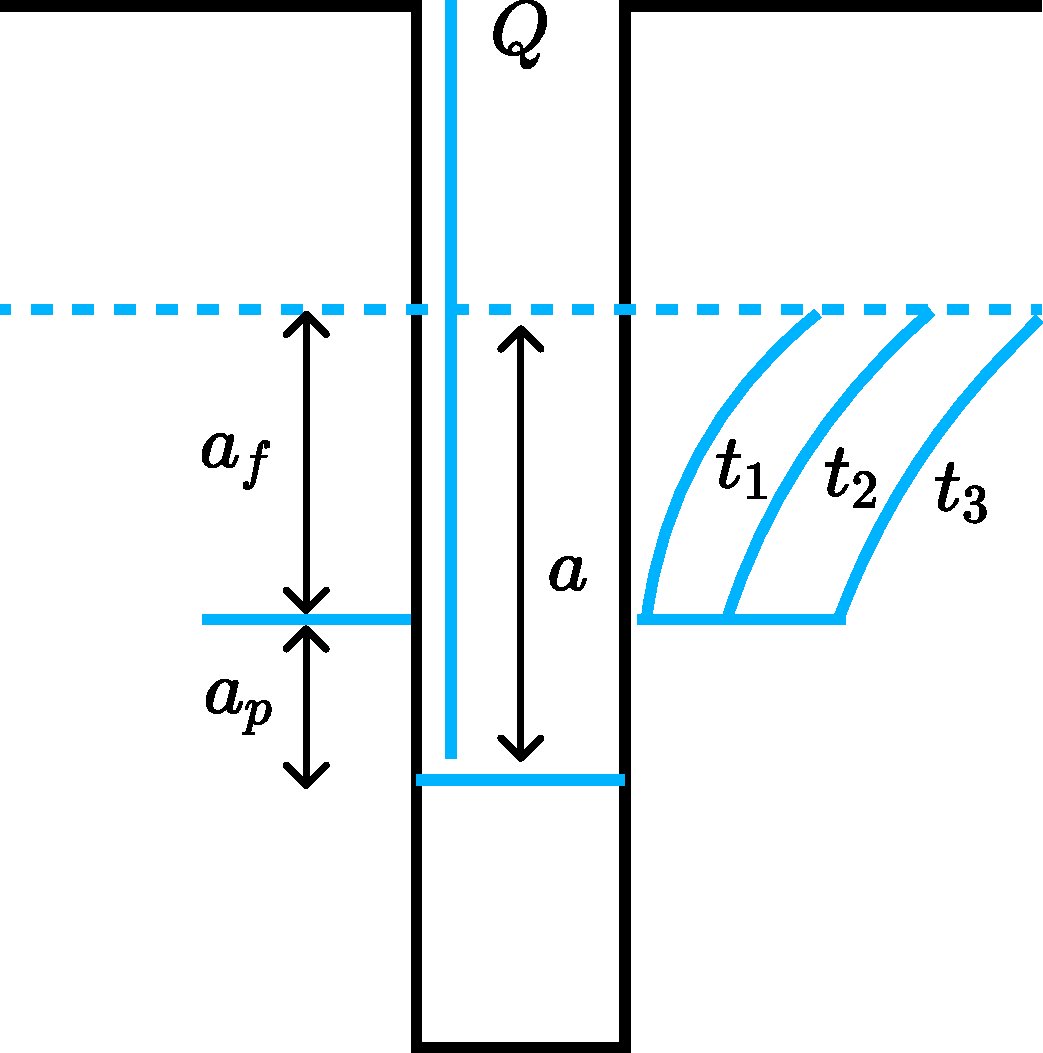
\includegraphics[width=0.5\textwidth]{gh32.pdf}
  \caption{Prueba de Aforo en un pozo}
  \label{gh32}
\end{figure}
Las características de $Q-a$, se grafican para localizar el punto de inflexión
Componente lineal $Q_{explotacion}\leq 0.8 Q_{max}$ y la Componente curvo $Q_{explotacion}\in \left(0.75-1 \right)Q_{\text{punto de inflexion}}$

\subsubsection{Componentes del abatimiento}
\begin{figure}[h!]
\centering
  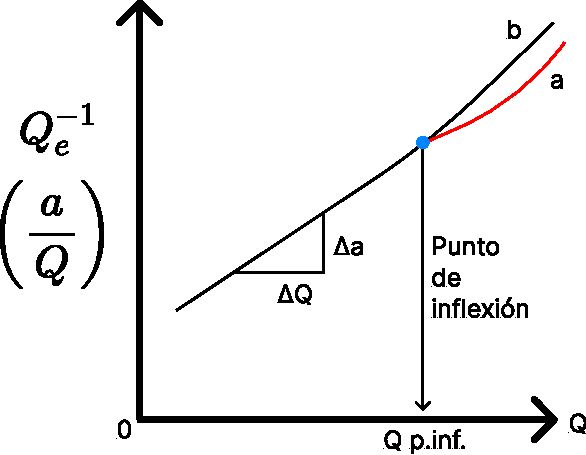
\includegraphics[width=0.5\textwidth]{gh34.pdf}
  \caption{Curva característica Q-a}
  \label{gh34}
\end{figure}
\begin{align*}
    &\frac{a}{Q} = \frac{BQ}{Q} + \frac{CQ^2}{Q}\\
    & Q_e^{ - 1} = B + CQ
\end{align*}
\begin{figure}[h!]
\centering
  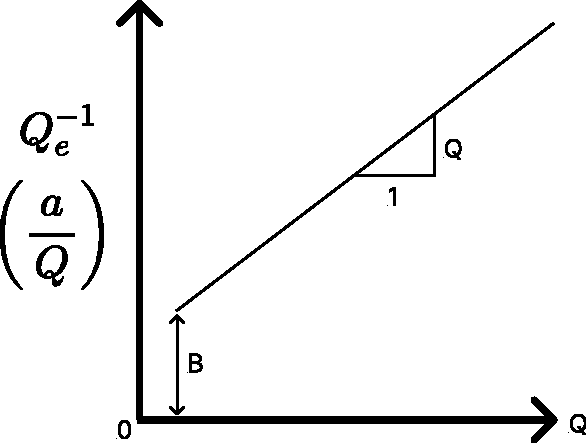
\includegraphics[width=0.5\textwidth]{gh33.pdf}
  \caption{Curva característica $Q-Q_e^{-1}$, donde $R^2\in (0.75,0.9)$}
  \label{gh33}
\end{figure}
\begin{align*}
    &a_f = BQ_{\exp}\\
    &a_p = CQ^2_{\exp }
\end{align*}
\subsubsection{Eficiencia del pozo}
\begin{align*}
    &\nu = \frac{a_f}{a_f +a_p }\times 100\\
    &\nu = \frac{BQ_{\exp }}{BQ_{\exp } + CQ^2_{\exp }} \times 100\\
    &Q_e = \frac{Q_{\exp }}{BQ_{\exp } + CQ^2_{\exp } }\implies T
\end{align*}
Finalmente, el gasto de explotación futura es:
\begin{equation}
    Q_e=\frac{Q_{exp}}{a_t}
\end{equation}
\section{Hidráulica de Pozos}
La hidráulica de pozos es una de las materias más importantes de la geohidrología, ya que proporciona las bases teóricas para interpretar las fluctuaciones de los niveles freáticos o piezométricos, provocados por la extracción de agua mediante pozos. Los prolbemas que estudia la hidráulica de pozos son muy diversos, entre los cuales se encuentran los siguientes:
\begin{itemize}
    \item \textbf{Identificación de los sistemas de flujo y determinación de sus características hidráulicas del acuífero}: La identificación del sistema de flujo que se trata (confinado, semiconfinado, libre) y la detminación de sus características hidráulicas (transmisividad, coeficiente de almacenamiento, permeabilidad) son esenciales para estudiar el comportamiento del acuífero. Como por ejemplo prever el comportamiento de los niveles de agua bajo diferentes regímenes de bombeo, cuantificar el volumen aprovechable de un acuífero, desarrollar modelos de simulación de acuíferos
    \item \textbf{Diseño de campos de bombeo}: El problema consiste en definir el número de distribución y régimen de operación de los pozos necesarios para la extracción de un caudal total definido
    \item \textbf{Definir el régimen de operación de pozos, dada una restricción en el abatimiento de los niveles}: Específicamente, en un acuífero costero el problema es descender a más del nivel del mar, por el riesgo de intrusión salina
    \item \textbf{Drenaje vertical}: En ocasiones, la geología subterránea es tal que los drenes verticales resultan más eficientes que los horizontales. En ese caso la hidráulica de pozos aporta las herramientas necesarias para diseñar el sistema de drenaje, ya sea en terrenos agrícolas o en zonas urbanas donde los niveles son someros
    \item \textbf{Recarga artificial}: Uno de los métodos utilizados para recargar un acuífero consiste en la inyección de agua a través de pozos. Conocidas las características del sistema acuífero, puede deducirse la capacidad de absorción de uno o varios pozos y predecirse la respesta a los niveles en función de la recarga.
\end{itemize}
Las pruebas de bombeo consisten en observar los efectos provocados (Abatimientos) en la superficie freática o piezométrica de un acuífero por la extracción de un caudal conocido. Los efectos (abatimientos) son registrados en el pozo de bombeo y pozos próximos a él.

La selección del sitio de prueba en ocasiones está obligado a problemas de carácter local o por interés de conocer las características hidráulicas del acuífero en un sitio específico, para estos casos un estudio geohidrológico, permite cierta flexibilidad para elegir el sitio de prueba, aunque lo más frecuente es que tengan que utilizarse pozos ya existentes Si en el área de interés hay varios pozos utilizables para el propósitos del que se trata, deben considerarse los siguientes aspectos:
\subsubsection{Requisitos para prueba de bombeo} 
\begin{enumerate}
    \item El equipo de bombeo debe encontrarse en condiciones apropiadas para sostener un caudal constante durante la prueba
    \item Facilidad para medir la profundidad al nivel del agua
    \item Que el caudal de extracción pueda ser fácilmente aforado
    \item No debe infiltrarse el agua bombeada del acuífero en las proximidades del pozo
    \item Conocer las características constructivas y el corte litológico del pozo
    \item Evitar la operación de los pozos próximos durante la prueba
\end{enumerate}
Para la interpretación completa de una prueba, lo ideal es contar con uno o varios pozos deobservación dispuestos a diferentes distancias del pozo de bombeo. Cuándo esto es posible, las características reducidas son más confiables y representativas de un área mayor. Por ello es muy recomendable disponer al menos de un pozo de observación.

Para la ubicación de pozos de observación con respecto al de bombeo, no hay una regla fija que indique la distancia a que debe situarse, ya que esta depende de las condiciones locales particulares de cada caso. En términos generales, el emplazamiento de los pozos de observación \textbf{a distancias entre 30 y 100 metros} del pozo de bombeo, es adecuado en la mayoría de los casos, aunque para una ubicación más cuidadosa debe contemplarse los aspectos siguientes: El tipo y la transmisividad del acuífero, el caudal de descarga, la ubicación y longitud del cedazo del pozo de bombeo.
\subsubsection{Profundidad de los pozos de observación}
Debe cuidarse que estos capten el mismo acuífero que está siendo bombeado. Cuando el pozo de bombeo capta la mayor parte del espesor del acuífero, y este es más o menos homogéneo, no es necesario que los pozos de observación penetren totalmente al acuífero, siendo suficiente un cedazo de longitud de preferencia ubicado a la profundidad en que se encuentra la parte media del cedazo del pozo de bombeo.
\subsubsection{Duración de la prueba de bombeo}
La duración recomendable de una prueba de bombeo depende de las características del sistema acuífero estudiado y de la precisión con que se desea conocer sus características hidráulicas, una prueba de larga duración tiene varias ventajas: las características deducidas de su interpretación son representativas de un área mayor, ya que los efectos del bombeo se propagan a mayor distancia, en algunos casos, se alcanza la estabilización del cono de abatimiento, facilitando la interpretación de la prueba.

La duración recomendable es de varias horas a varios días, siendo conveniente prolongarla tanto como sea posible, sobre todo cuando se cuenta con pozos de observación, en caso contrario, no se justifica realizar pruebas largas, en general son suficientes unas cuantas horas de bombeo.
\subsubsection{Cómo se realiza la prueba de bombeo}
Antes de iniciar la prueba, se revisará el equipo a utilizar (Cronómetros, sondas, cintas métricas, escuadras de aforo, otros). Para verificar su correcto funcionamiento seguidamente se llevarán a cabo las siguientes actividades:

\begin{enumerate}
    \item Antes de iniciar el bombeo, se medirá la profundidad del nivel estático en el pozo de bombeo y en el (o los) pozos de observación. Se anotará la hora de inicio de la prueba y las lecturas iniciales con el nombre de los pozos a que correspondan
    \item Se iniciará el bombeo procurando mantener un caudal constante, y se procederá a medir la profundidad al nivel del agua en el pozo de bombeo y en el o los pozos de observación a los tiempos establecidos en el formato respectivo (1,2,4,8,15,30,45 min, 1,2,4,8 Hrs.)
    \item A intervalos de tiempos seleccionados, se harán las lecturas necesarias para cuantificar el caudal de bombeo (Métodos de aforo)
    \item Con las observaciones realizadas, se construirá en el sitio de la prueba, la gráfica de variación del nivel dinámico en el tiempo para el pozo de bombeo y para uno de los pozos de observación.
    \item La duración de la etapa de bombeo fijada inicialmente, como ya se indicó podrá modificarse con el siguiente criterio: \begin{enumerate}
    \item Su el caudal de bombeo varía apreciablemente, en forma continua e incontrolable, se suspenderá la prueba
    \item Cuando en la gráfica de nivel dinámico-tiempo del pozo de bombeo, se observe una estabilización del nivel dinámico en un tiempo menor de cuatro horas
    \end{enumerate}
\end{enumerate}
De todo lo expuesto se despende que una prueba de bombeo requiere una cuidadosa programación e implica un gasto económico más o menos considerable. Desde luego, la duración del bombeo y el número de pozos de observación recomendables en cada caso particular depende del tipo de problema de que se trate.

Las pruebas de bombeo a gasto constante pueden ser en Régimen permanente o Régimen variable; y estas últimas en descenso (bombeo) o en recuperación.

subsubsection{Régimen transitorio (variable) y estacionario (permanente)}
Cuando se inicia el bombeo en un pozo, se extrae agua de la formación acuífera próxima a él. AL originarse un gradiente hidráulico el agua en las zonas contiguas comienza a verter en el interior del pozo. Se ha iniciado un cono que evoluciona a lo largo del tiempo y del espacio. Esta variación viene motivada porque el acuífero cede parte de su almacenamiento, en tales circunstancias se dice que el régimen es transitorio o variable.

Puede llegar el caso en que el agua extraída sea igual a una cantidad que sea aportada por una recarga cercana. En este caso el acuífero deja de aportar de su almacenamiento para convertirse en un transmisor. En estas condiciones se dice que se ha alcanzado un régimen estacionario o permanente (o equilibrado). Se comprenderá que cuando iniciamos el bombeo, normalmente nos encontramos en condiciones transitorias, con el tiempo se puede alcanzar el otro régimen (estacionario).

Cuando se extrae cierto gasto, el nivel de referencia disminuye, formando un gradiente hidráulico ,fluyendo el agua de una carga mayor a una carga menor.

Los niveles del cono y dentro del pozo descienden porque el gasto que extrae la bomba es tomado del almacenamiento del acuífero. Mientras el cono (los abatimiento) se estén moviendo en el tiempo, $\frac{d\,Ab}{dt}\neq 0$
\subsubsection{Teoría del regimen estacionario}
Los trabajos de J. Dupuit (1863) constituyen la base del estudio dinámico de las aguas subterráneas en las proximidades de la captación, en régimen estacionario. G. Thiem aplicando las hipótesis de Dupuit obtuvo en 1906, una expresión de flujo que se parece a la de este autor, por lo que se le designa con el nombre de la fórmula de Dupuit-Theim.

La hipótesis básicas de la ecuación de Dupuit-Thiem son las siguientes:
\begin{enumerate}
    \item El acuífero es homogéneo, infinito e isótropo y el agua es de densidad y viscosidad constantes
    \item Se cumplen las condiciones de la ley de Darcy
    \item Como consecuencia de la homogeneidad e isotropía, el coeficiente de almacenamiento es constante
    \item El espesor del acuífero es constante y su base horizontal
    \item El pozo es ideal, esto es, radio mínimo, no existe pérdida de carga en el paso de agua de la formación acuífera al interior de este, su caudal es constante y es totalmente penetrante
    \item El flujo es radial
    \item No hay variación del nivel dinámico en el tiempo ($\frac{da}{dt}=0$)
\end{enumerate}
\subsubsection{Regimen estacionario en acuífero confinado}
En acuífero confinado, alineados con el pozo de bombeo, hay dos pozos de observación 1 y 2 a distancias $r_1$ y $r_2$ de P.B. Si es $b$ el espesor del acuífero, el cual se considera constante. Por continuidad, el caudal que se filtra por la superficie lateral de un cilindro de radio $r$ concéntrico con el pozo, es el mismo caudal bombeado Q. Aplicando la fórmula de Darcy a este cilindro, tendríamos que:
% imagen
\begin{equation}
    Q = K \frac{dh}{dr} 2 \pi r b
\end{equation}
Separando variables e integrando:
\begin{align*}
    &\int_{r1}^{r2} \frac{dr}{r} = \frac{2 \cdot \pi kb }{Q} \int_{h1}^{h2} dh\\
    &\ln{\frac{r_2}{r_1}} =  \frac{2 \cdot \pi Kb }{Q}\left(h_2 - h_1 \right)
\end{align*}
Como $h_2-h_1=a_1-a_2$
\begin{align*}
    &K = \frac{Q}{2 \cdot \pi b\left(a_1 - a_2 \right)} \ln{\frac{r_2}{r_1}}\\
    &T = \frac{Q}{2 \cdot \pi \left(a_1 - a_2 \right)} \ln{\frac{r_2}{r_1}}
\end{align*}
Esta última expresión para cuando se cuenta con dos pozos de observación. Si se cuenta con un sólo pozo de observación (que por cierto es más frecuente), por analogía se podrá utilizar la expresión siguiente
\begin{equation}
    T= \frac{Q}{2 \pi \left(a_p - a_1 \right)}\ln{\frac{r_1}{r_p}}
\end{equation}
Se debe considerar con reserva el valor obtenido por esta última expresión ya que el abatimiento en el pozo $a_p$ está afectado por las pérdidas de carga debidas al paso del agua del acuífero al interior del pozo

Si se define radio de influencia (R) como la distancia del pozo de bombeo al punto donde el abatimiento se hace cero. Así en $r_1=R$, $a_1=0$ entonces la expresión queda:
\begin{equation}
    T= \frac{Q}{2 \pi a_p} \ln{\frac{R}{r_p}}
\end{equation}
La ecuación del cono de abatimiento será entonces $a= a(r), r\in \left(r_p,R\right)$
\begin{equation}
    a = \frac{Q}{2 \pi T}\ln{\frac{R}{r_a}}
\end{equation}

Con estas fórmulas se puede relacionar los abatimientos, gastos, transmisividades y distancias de los puntos que definen el cono de abatimiento. Hay que considerar que cuando no se tienen pozos de observación se ha de trabajar con el radio del pozo y el abatimiento en el pozo (el cual no es real ya que está afectado por las pérdidas de carga debidas al pasar el agua al interior del pozo) Y radio de influencia. Al no conocerse el radio de influencia, tendrá que estimarse de alguna forma.
\begin{problem}[Datos: b= 24m, gasto de 47lps, $a_p= 3.5m$, $r_p= 10^{\prime\prime}$, $a_1= 0.18m$, $r_1=356m$]
\textit{ Sol. }

Se tiene que $T= 0.163 m^s/s$, porque $T=kb$, además $Q_e=Q/a= 13.4 lps/m$. Aunado se tiene que $K=6.8\times 10^{-4} m/s$ (material: Grava-arena, arena)

$S=x$ puesto que $a= \frac{Q}{2\pi T}\ln{\frac{R}{r}}$ entonces $R=527$
    
Volumen de acuífero = $\pi r^2\cdot b= \pi\left(527m\right)^2\cdot 24m= 20,940,322 m^3$

Si se tuviera la eficiencia hidráulica del pozo (válido si no ha pasado más de un año), se Podría corregir o afinar el abatimiento del POZO debido a las pérdidas de carga por construcción del pozo.
\end{problem}
\subsubsection{Régimen estacionario en acuífero libre}
El problema que presentan los acuíferos libres es que dejan de cumplir una de las condiciones impuestas a la ecuación general; siendo tal condición el que el flujo deje de ser radial, presentándose componentes verticales de velocidad\dots

Si se considera mínimo el efecto de esta condición, se puede dar un tratamiento similar a la solución del problema en el acuífero confinado

Alternativamente, es posible solucionar el problema aplicando la simplificación de Dupuit. La cual consiste en hacer corrección de los abatimientos medios tanto en pozo de bombeo como en pozos de observación, cuando estos sean igual o superen el 15\% del espesor saturado inicial del acuífero libre; e interpretar la prueba de bombeo como si se tratara de un acuífero confinado
\begin{equation}
    a_c = a - \frac{a^2}{2b}
\end{equation}
En el acuífero libre, alineados con el pozo de bombeo, hay dos pozos de observación 1 y 2 a distancias $r_1$ y $r_2$. Estas condiciones presenta la figura siguiente:

Por continuidad, el caudal que se filtra por la superficie lateral de un cilindro de radio $r$ concéntrico con el pozo, es el mismo caudal bombeado Q. Aplicando la ley de Darcy a este cilindro, para condiciones libres, tendremos que:
\begin{align*}
    &Q= kiA\\
    &Q= 2\pi r h K\left(\frac{dh}{dr}\right)
\end{align*}

Separando variables
\begin{equation*}
    \int \frac{dr}{r}= \frac{2\pi K}{Q} \int h \, dh
\end{equation*}

integrando:
\begin{align*}
    &\int_{r1}^{r2} \frac{dr}{r} = \frac{2\pi K}{Q} \int_{h1}^{h2} h\,dh\\ 
    &\ln{\frac{r_2}{r_1}} = \frac{2\pi K}{Q} \left(\frac{h^2_2 - h^2_1 }{2}\right)\\
    &K = \frac{Q}{\pi\left(h^2_2 - h^2_1\right)} \ln{\frac{r_2}{r_1}}
\end{align*}
Obsérvese que no es posible la obtención de T ya que b es variable. 

\begin{problem}[Teniendo la siguiente figura]
    
\textit{ Sol. }

$K=\frac{Q}{\pi\left(h^2_2- h^2_1\right)} \ln{\frac{r_2}{r_1}}= 2.163\times 10^{-4} m/s$, luego $T=kb=0.0138 m^2/s$. Entonces $h_2= 135-71.2= 63.8m$ $r_1=9^{\prime\prime}$

El $a_p= 3.67m$ no supera el 15\% de b, interpretando como si se tratara de un acuífero confinado:
\begin{equation*}
    T = \frac{Q}{2\pi \left(a_p - a_1 \right)} \ln{\frac{r_1}{r_p}}= \frac{0.053}{2\pi \left(3.67 - 0\right)} = \frac{0.0134m^2}{s}
\end{equation*}

Luego b= 63.8m y $K= 2.101\times 10^{-4}$. La diferencia porcentual es de 3\%. El volumen del acuífero es de $ 3.1416\cdot 78^2\cdot 63.8= 1,219,440.9m^3$
\end{problem}

\subsection{Teoría del régimen transitorio en acuíferos confinados}
Uno de los hechos más notables en el conocimiento de la hidráulica subterránea fue hecho por C.V. Theis el cual basándose en la analogía de flujo de calor en medios homogéneos, desarrolló en 1935, la fórmula que expresa el descenso del nivel en un pozo de observación, en función del tiempo de duración del bombeo, desde las condiciones de reposo. Posteriormente C.E. Jacob obtuvo las mismas fórmulas basándose  en conceptos exclusivamente hidráulicos.

Al sustituye la ley de Darcy en la expresión del principio de conservación de masa en un volumen de control diferencial, se obtiene:
\begin{equation}
    \frac{\partial }{\partial x} \left(K_x \frac{\partial h}{\partial x} \right) + \frac{\partial }{\partial y} \left(K_y \frac{\partial h}{\partial y} \right) + \frac{\partial }{\partial z} \left(K_z \frac{\partial h}{\partial z} \right) = \frac{S_s \partial h}{\partial t}
\end{equation}
Si se multiplica por el espesor del acuífero (b) y se sustituye $T=Kb$ y $b= S_s b$ se obtiene:
\begin{equation*}
    \frac{\partial }{\partial x} \left(T_x \frac{\partial h}{\partial x} \right) + \frac{\partial }{\partial y} \left(T_y \frac{\partial h}{\partial y} \right) + \frac{\partial }{\partial z} \left(T_z \frac{\partial h}{\partial z} \right) = \frac{S \cdot \partial h}{\partial t} 
\end{equation*}
Para un medio homogéneo e isótropo $Tx = Ty = Tz = T$, y se factoriza:
\begin{equation*}
    \frac{\partial }{\partial x} \left(\frac{\partial h}{\partial x} \right) + \frac{\partial }{\partial y} \left(\frac{\partial h}{\partial y} \right) + \frac{\partial }{\partial z} \left(\frac{\partial h}{\partial z} \right) = \frac{S \cdot \partial h}{T \cdot \partial t} 
\end{equation*}
La cual, para flujo radial y en coordenadas polares se convierte en:
\begin{equation*}
    \frac{\partial^2 h}{\partial r^2} + \frac{1}{r} \cdot  \frac{\partial h}{\partial r} = \frac{S}{T} \cdot \frac{\partial h}{\partial t} 
\end{equation*}
Las hipótesis que determinan la validez de las ecuaciones en régimen transitorio son las ya mencionadas para régimen permanente. Además, se considera que el agua que se bombea es extraída instantáneamente de la formación acuífera, no vuelve a entrar en ella y produce un inmediato descenso de nivel $\frac{da}{dt}\neq 0$

La solución de la ecuación diferencial anterior toma la forma de una integral exponencial,
que nos permite hallar el descenso en función del límite inferior de la integración: $a= f (Q , K, l , S , t)$
\begin{equation}
    a = \frac{Q}{4 \cdot \pi T} \int_{u}^{\infty} \frac{e^{ - u}}{u}\, du
\end{equation}
Donde $u=\frac{Sr^2}{rTt}$ cuya solución no es posible obtener analíticamente.

La solución de la integral (conocida como función de pozo W(u)) se obtiene mediante una serie de Taylor:
\begin{align*}
    &W(u) = \int_{u}^{\infty} \frac{e^{ - u}}{u}\, du = - 0.577216 - \ln{(u)} + \sum_{n = 1}^{\infty} \frac{-(-u)}{n\cdot n!}\\
    &\sum_{n = 1}^{\infty} \frac{ -( - u)^{n} }{n\cdot n!} = u - \frac{u^2}{2\cdot 2!} + \frac{u^3}{3\cdot 3!} - \frac{u^4}{4\cdot 4!} + \dots \\ 
    &a = \frac{Q}{4\pi T}\left( - 0.577216 - \ln{(u)} + u - \frac{u^2}{2\cdot 2!} + \frac{u^3}{3\cdot 3!} - \frac{u^4}{4\cdot 4!} + \dots \right)
\end{align*}
\begin{align}
    &a = \frac{Q}{4\pi T} W(u)\\ 
    &u = \frac{S_r^2}{4Tt}
\end{align}
\begin{figure}[h!]
\centering
  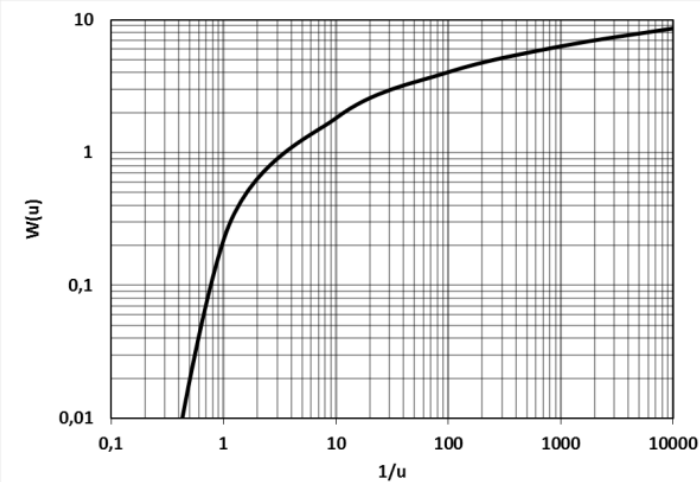
\includegraphics[width=0.9\textwidth]{gh34.png}
  \caption{Función de pozo Theis en acuíferos confinados, pozos penetrantes}
  \label{gh34png}
\end{figure}
\subsection{Método Gráfico-Numérico de Theis}
Con base en esa ecuación, desarrolló el método gráfico-numérico para obtener los parámetros T y S que a continuación describe:

\begin{enumerate}
    \item Trazar la curva tipo (curva de la función de pozo o de Theis) 1/u- W(u), en papel doble logarítmico
    \item Dibujar la gráfica tiempo-abatimiento (curva de campo t,a) del pozo de observación en papel doble logarítmico del mismo módulo
    \item Suponer las gráficas manteniendo los ejes paralelos, y buscar la coincidencia de la curva de campo y la curva tupo (dando preferencia a los puntos de tiempos mayores)
    \item Seleccionar un punto de ajuste y obtener sus coordenadas tanto en la curva de campo ($t_p,a_{pt}$) como en la curva tipo ($(1/u)_{pt}, W(u)_p$). De preferencia con coordenadas cerradas en alguna de las dos curvas
    \item Sustituir las coordenadas en las expresiones siguientes:
    \begin{align*}
        T = \frac{Q}{4\pi a_p}&& S = \frac{4Tt_p}{\left(\frac{1}{u}\right)_p r^2}
    \end{align*}
\end{enumerate}
$r$ es la distancia del centro del pozo de bombeo al pozo de observación.

Se puede demostrar que los valores de T y S son los mismos para cualquier punto de ajuste.
\begin{example}
    Se realizaron mediciones de niveles dinámicos en el pozo de bombeo y en un pozo de observación a 100m de distancia. El gasto de la prueba es de 150lps y el espesor del acuífero es de 580 metros.
    \begin{longtable}[c]{@{}ccc@{}}
        \toprule
        Tiempo (min) & Abatimiento (m) en OB & Abatimiento (m) en PO \\* \midrule
        \endfirsthead
        %
        \endhead
        %
        \bottomrule
        \endfoot
        %
        \endlastfoot
        %
        1            & 2.2                   &                       \\
        2            & 5.5                   &                       \\
        3            & 8.21                  &                       \\
                     & 10.11                 &                       \\
        5            & 12.22                 &                       \\
        6            & 13.31                 &                       \\
        8            & 16.11                 &                       \\
        10           & 17.9                  &                       \\
        15           & 22.1                  &                       \\
        20           & 25.02                 &                       \\
        25           & 27.1                  &                       \\
        30           & 28.05                 &                       \\
        40           & 30.01                 &                       \\
        50           & 31.98                 & 0.2                   \\
        60           & 32.5                  & 0.4                   \\
        70           &                       & 0.6                   \\
        80           & 37.9                  & 0.85                  \\
        90           &                       & 1                     \\
        100          & 39.85                 & 1.4                   \\
        120          & 40.5                  & 1.95                  \\
        150          & 44                    & 2.8                   \\
        200          & 47                    & 4.2                   \\
        300          & 51                    & 6.6                   \\
        400          & 54.8                  & 8.55                  \\
        600          & 57.2                  & 11.8                  \\
        800          & 61.4                  & 14                    \\
        1200         & 62.8                  & 17.9                  \\
        2000         & 37.8                  & 22.6                  \\
        3000         & 72.4                  & 26.5                  \\
        4000         & 75                    & 29                    \\
        6000         & 77.8                  & 32.5                  \\* \bottomrule
        \caption{Prueba de bombeo}
        \label{tabgh11}\\
        \end{longtable}
\end{example}
\textit{ Sol. }
% Graficar
Después de suponer la curva de los datos de campo a la función de pozo se obtuvieron las coordenadas de los puntos de ajuste tanto para los datos del pozo de bombeo como para los del pozo de observación. Para el pozo de bombeo:
\begin{align*}
    t = 1min&& W(u) = 1 && a = 10m && \frac{1}{u} = 0.97
\end{align*}
Sustituyendo en las ecuaciones:
\begin{align*}
    &T = \frac{Q}{4\pi a_p } W(u)_p = \frac{0.150}{4 \pi (10)}(1) = 0.001194 \frac{m^2}{s}\\
    &K = \frac{T}{b} = \frac{0.01194 \frac{m^2}{s}}{580m}  = 2.06 \times 10^{ - 6} \frac{m}{s}\\
    &S = \frac{4Tt_p}{\left(\frac{1}{u}\right)_p r^2} = \frac{4\left(0.001194 \frac{m^2}{s}\right) 1 \cdot 60}{0.97 (0.33m)^2} = 2.71
\end{align*}
Para pozo de bombeo:
\begin{align*}
    t = 20min&& W(u) = 0.3 && a = 3m && \frac{1}{u} = 20
\end{align*}
\begin{align*}
    &T = \frac{Q}{4\pi a_p } W(u)_p = \frac{0.150}{4 \pi (3)}(0.3) = 0.00119 \frac{m^2}{s}\\
    &K = \frac{T}{b} = \frac{0.0119 \frac{m^2}{s}}{580m}  = 2.05 \times 10^{ - 6} \frac{m}{s}\\
    &S = \frac{4Tt_p}{\left(\frac{1}{u}\right)_p r^2} = \frac{4\left(0.00119 \frac{m^2}{s}\right) 20 \cdot 60}{0.97 (0.33m)^2} = 
\end{align*}
Los resultados se ven afectados por las pérdidas de carga de construcción del pozo, dando coeficientes de almacenamiento atípicos para el acuífero confinado.
\subsection{Simplificación de Jacob}
En la función de pozo, al crecer el tiempo transcurrido (t) desde el comienzo del bombeo, $u=\frac{Sr^2}{4Tt}$  decrece inversamente con el tiempo. En el desarrollo en serie de la función de pozo, Jacob comprobó que después de un tiempo relativamente corto a partir del comienzo del bombeo, los valores de los términos en serie de potencias se hacían tan rápidamente decrecientes que podrían perfectamente despreciarse a partir de ciertos valores del tiempo ($ t= 2.5r^2S/T, u= 0.1$). Por lo tanto, Jacob propuso la simplificación de la fórmula de Theis, a partir de cierto intervalo después del comienzo del bombeo, despreciando en el desarrollo en serie de W(u), todos los términos a partir del segundo y dejándola convertida en:

Solución de Theis:
\begin{align}
    &a = \frac{Q}{4\pi T}W(u)\\
    &W(u) = - 0.577216 - \ln{\left(u\right)} + \sum_{n = 1}^{\infty} - \frac{ -( -u)^2}{n \cdot n!}\\
    &u = \frac{Sr^2}{4Tt}\\
    &u\leq 0.1\implies \sum_{n = 1}^{\infty} - \frac{ -( -u)^2}{n \cdot n!} \to 0\\
    &W(u) = - 0.577216 - \ln{(u)}\\
    &a = \frac{Q}{4\pi T}\left( -\ln{(u)} - 0.577216 \right)\\
    &t\geq \frac{2.5S \cdot r^2}{T}\\
    &\ln{\left(\frac{4Tt}{Sr^2}\right)} - \ln{e^{0.577216}}\\
    &\ln{\left(\frac{2.25Tt}{Sr^2}\right)}
\end{align}
Y por lo tanto la ecuación simplificada de Jacob Cooper es:
\begin{equation}
    a = \frac{2.3Q}{4\pi T}\cdot \log{\left(\frac{2.25 \cdot T \cdot t}{Sr^2}\right)}
\end{equation}
si se grafica en una escala logarítmica abatimiento de tiempo y aritmética de hacia abajo
\begin{enumerate}
    \item Con los datos de la prueba de bombeo se grafican, con $x= \log{t}/ abatimiento$ en escala semi $log(t)/a$
    \item Ajustar los datos de la prueba a una línea recta, dando preferencia a los tiempos mayores
    \item Se toman los puntos iniciales y finales de la curva $(p_1,a_1),\, (p_2,a_2)$
    \begin{align}
        &p_1;a_1 = \frac{2.3Q}{4\pi T} \cdot \log{\left(\frac{2.25STt_1}{Sr^2}\right)}\\
        &p_2;a_2 = \frac{2.3Q}{4\pi T} \cdot \log{\left(\frac{2.25STt_2}{Sr^2}\right)} 
    \end{align}
    Por lo tanto:
    \begin{align*}
        &a_2 - a_1 = \frac{2.3Q}{4\pi T}\left[\log{\left(\frac{2.25STt_2}{Sr^2}\right)} - \log{\left(\frac{2.25STt_1}{Sr^2}\right)} \right]\\
        &a_2 - a_1 = \frac{2.3Q}{4\pi T}\log{\frac{t_2}{t_1}} = Pendiente\\
        &a_2 - a_1 = \frac{2.3Q}{4\pi T} \cdot P \implies T = \frac{2.3Q}{4\pi P} = 0.183 \frac{Q}{P} 
    \end{align*}
    \begin{equation}
        T = 0.183 \frac{Q}{P}
    \end{equation}
    \item Tomando un punto $t_0$ que corta la eje x, sustituyendo obtendríamos:
    \begin{align*}
        0 = \frac{2.3Q}{4\pi T} \log{\left(\frac{2.25Tt_0}{Sr^2}\right)} 
    \end{align*}
    como necesitamos que el numerador del logaritmo sea igual a $Sr^2$, entonces basta con igualarlo, obteniendo que S=
    \begin{equation}
        S = \frac{2.25Tt_0}{r^2}
    \end{equation}
    \item Ya ajustados los datos de la recta, ahora se obtiene la pendiente de la recta $P$ en $\frac{m}{1\, ciclo}$, $t_0$ es el punto donde el abatimiento vale 0
    \item Ajuste por tiempo de validez: teniendo T y S, se sustituye en la ecuación $t=\frac{Sr^2}{T}$, por lo que se ajusta la pendiente de la recta. 
\end{enumerate}
Teniendo que $T= 0.00124$ y $S= 0.00303$, en 6,000 minutos (t=6000*60seg) es:
\begin{equation}
    R = \frac{3}{2} \sqrt{\frac{Tt}{S}} = 575.7m
\end{equation}
Con una pendiente de 0.81, tenemos:
\begin{align*}
&0.81ln(t)-0.439=0\\
&0.81ln(t)= 0.439\\
&ln(t)= 0.439/0.81\\
&t= e^(0.439/0.81) = 1.7191
\end{align*}
% ?
\subsubsection{Método de Jacob para un pozo de observación}
Para un pozo de observación la distancia ``r'' al pozo de bombeo, Q, T y S son constantes, por lo tanto, para dos medidas de abatimiento $a_1$ y $a_2$ en los $t_1$ y $t_2$, de una prueba de bombeo, se obtendrá:
\begin{align*}
    P_1:a_1 = \frac{Q}{4 \pi T}\left(\ln{\left(\frac{4Tt_1}{Sr^2}  - 0.577216 \right)}\right)\\
    P_2:a_2 = \frac{Q}{4 \pi T}\left(\ln{\left(\frac{4Tt_2}{Sr^2}  - 0.577216 \right)}\right) 
\end{align*}
Si se restan los abatimientos, la expresión queda como:
\begin{align*}
    &a_2 - a_1= \frac{Q}{4\pi t}ln{\left(\frac{t_2}{t_1}\right)}\\
    &a_2 - a_1 = \frac{2.302585093Q}{4 \pi T} \log{\left(\frac{t_2}{t_1}\right)}
\end{align*}
A partir de esta expresión desarrollo el método simplificado de interpretación de pruebas de bombeo en acuíferos confinados con un pozo de observación (que es lo más común), que consiste en lo siguiente:
\begin{enumerate}
    \item Construir la gráfica de tiempo (escala logarítmica) contra abatimiento (escala aritmética) de los datos de la prueba de bombeo.
    \item Ajustar a una recta los puntos que se alinean y determinar su pendiente. Los puntos que se recomienda dar más importancia para el ajuste son los de tiempos más grandes, así los puntos de tiempos cortos se salen frecuentemente de la recta de ajuste, debido a que es para los puntos donde no es válida la simplificación de Jacob.
    \item Tomar dos puntos de la recta, en el inicio y final de un ciclo logarítmico. Para estos puntos la expresión se reduce a:
    \begin{equation}
        P = a_2 - a_1 = \frac{2.3Q}{4 \cdot \pi T} \cdot \log{\left(\frac{10^{n + 1 }}{10^n}\right)} = \frac{2.3Q}{4 \pi T}
    \end{equation}
    
    Entonces $a_2- a_1 = P$ ( pendiente de la recta en metros de abatimiento por ciclo logarítmico).
    
    Y la transmisividad podrá obtenerse mediante la expresión siguiente:
    \begin{equation}
        T = \frac{2.302585093Q}{4\pi P} = 0.183 \frac{Q}{P}
    \end{equation}
    \item A partir del valor de T se puede determinar el coeficiente de almacenamiento. Si se prolonga la recta hasta a=0, tenemos un t=t . La ecuación simplificada de Jacob toma el valor de:
    \begin{equation}
        0 = \frac{Q}{4\pi T} \left(\ln{\left(\frac{4Tt_0}{Sr^2}\right)} -0.577216 \right)
    \end{equation}
    Lo que implica que lo que se encuentra dentro del paréntesis vale cero, entonces:
    \begin{align*}
        \ln{\frac{4Tt_0}{Sr^2}} = 0.577216\\
        \frac{4Tt_0}{Sr^2} = e^{0.577216} =1.773\\
        S = \frac{4Tt_0}{1.773r^2} = 2.25 \cdot \frac{Tt_0}{r^2}
    \end{align*}
\end{enumerate}

\subsubsection{Método simplificado de Jacob con varios pozos de observación}
\begin{equation}
    a = \frac{2.3 Q}{4\pi T} \log{\frac{2.25T \cdot t}{S \cdot r^2}} 
\end{equation}
Las constantes son $Q,T,S,t$, y las variables serán $a$ y $r$.
En la práctica, se interpreta una fotografía en mínimo dos pozos de observación.
\begin{align*}
    &a_1 = \frac{2.3Q}{4\pi T}\log{\left(\frac{2.25Tt}{Sr_1^2}\right)}\\
    &a_2 = \frac{2.3Q}{4\pi T}\log{\left(\frac{2.25Tt}{Sr_2^2}\right)}\\
    &P = a_1 - a_2 = \frac{2.3Q}{4\pi T} \cdot \log{\frac{r^2_2}{r^2_1}}\\
    &T = \frac{2(2.3)}{4\pi} \frac{Q}{P} = 0.366 \frac{Q}{P}\\
    &\therefore T = 0.366 \frac{Q}{P}
\end{align*}
Entonces $r_0$ es el radio de influencia
\begin{align*}
    &0 = \frac{2.3Q}{4\pi T} \log{\frac{2.25Tt}{Sr_0^2}}\\
    &S = \frac{2.25Tt}{r_0^2}\\
    &\therefore R = \frac{3}{2}\sqrt{\frac{Tt}{S}}\\
\end{align*}
\subsubsection{Régimen transitorio en acuíferos libres}
Los acuíferos libres se caracterizan por estar  limitados superiormente por una superficie freática, puesto que el espesor del acuífero varía con las fluctuaciones de esta superficie, la transmisividad del acuífero es también variable en el área en el tiempo, en las cercanías de un pozo de bombeo en operación. Si la fluctuación del nivel es poco significativa ocn respecto al espesor del acuífero, la transmisividad puede suponerse contante y la interpretación de las pruebas de bombeo se efectúa como si tratara de un acuífero confinado. En cambio su duchas fluctuaciones son importantes especialmente iguales o mayores a 155 del espesor saturado del acuífero, los abatimientos medidos se corrigen mediante la fórmula de corrección de Dupuit:
\begin{equation}
    a_c= a-\frac{a^2}{2b}
\end{equation}
Los abatimientos así obtenidos se interpretan con los métodos para acuíferos confinados.
\begin{example}
En una prueba de bombeo, se mantuvo el gasto constante de 23.1lps, los abatimientos se midieron en un pozo de observación a 10m del pozo de bombeo, se sabe por datos de la perforación que el acuífero es libre, con espesor saturado inicial de 5m. Determine la transmisividad y coeficiente de almacenamiento por el método simplificado de Jacob.

Como se observa en los datos de la prueba, el abatimiento máximo en la misma rebasa el 15\% del espesor saturado inicial, por lo que los abatimientos se corrigen, y la prueba se interpreta como si se tratara de un acuífero confinado.
\begin{table}[h!]
    \centering
    \begin{tabular}{@{}ccc@{}}
    \toprule
    t(min) & Abat. (m) & Abat. Corr (m) \\ \midrule
    1      & 0         & 0              \\
    10     & 0.024     & 0.0239         \\
    30     & 0.018     & 0.0179         \\
    50     & 0.310     & 0.3003         \\
    100    & 0.520     & 0.4926         \\
    300    & 1         & 0.9            \\
    100    & 1.38      & 1.1895         \\
    10,000 & 2.3       & 1.771          \\ \bottomrule
\end{tabular}
\caption{Interpretación cuando $Q=23.1lps$, $r=10m$, el acuífero es libre y $b=5m$}
\label{tabgh12}
\end{table}
\end{example}
\textit{ Sol. }

Graficándolo, se obtiene un modelo $a=0.2782\ln{(t)}-0.7572$, con una $R^2=0.9937$ sin los primeros tres tiempos, así:
\begin{align*}
    &T= \frac{0.3183Q}{P}= \frac{0.183 \cdot 0.0231}{0.5564} = 0.00759 \frac{m^2}{s}\\
    &S_y = 2.25 \frac{Tt_0}{r^2} = 2.25 \frac{0.00759 \cdot 15.2 \cdot 60}{10^2} = 0.1567
\end{align*}
Este coeficiente de almacenamiento es propio de un acuífero libre. El tiempo a partir del cual es válida la aproximación de Jacob es: 
\begin{equation*}
    t = \frac{2.5 \cdot 0.1557 \cdot  10^2}{0.00759}= 5128.5 s= 85\min  
\end{equation*}
Viendo la gráfica, del tiempo en min, el radio de influencia para la duración de la prueba t= 10,000min = 6.944 días es:
\begin{equation*}
    R = \frac{2}{3} \sqrt{ \frac{7.59 \times 10^{ - 3} }{0.1557}}
\end{equation*}
% TODO: Sustituir chido los valores 
\begin{example}
    Se hizo una prueba en un pozo de bombeo que estaba extrayendo 37 lps, al interpretarlo, se obtuvo una transmisividad de $0.048m^2/s$ y el coeficiente de almacenamiento es $S= 6.7\times 10^{-4}$ (siendo un acuífero confinado)
\begin{enumerate}
    \item El tiempo de operación para que a 509m se tenga un abatimiento de 0.43m ¿En qué tiempo sucede esto?
    \item La distancia a la cual tiene efecto el bombeo (Radio de influencia)
    \item El abatimiento en el pozo si la eficiencia $eta= 48.5\%$
    \item El caudal específico
\end{enumerate}
\textit{ Sol. }

Mediante la simplificación de Jacob, 
\begin{equation*}
    a = \frac{Q}{4\pi T}\ln{\frac{2.25Tt}{Sr^2}}
\end{equation*}
Despejando la t:
\begin{equation*}
    t = \frac{r^2\cdot e^{\frac{a\cdot 4\pi T}{Q}}}{2.25T} = \frac{(509)^2 \left(6.7 \times 10^{ - 4}\right)}{2.25\left(0.018\frac{m^2}{s}\right)}\cdot e^{\frac{4\pi\cdot 0.43\cdot 0.018}{0.037\frac{m^3}{s}}} = 59,389.06
\end{equation*}
Siendo equivalente a 16 horas con 29.8 minutos.

El tiempo de validez $t= \frac{2.5 Sr^2}{T}$ y sustituyendo:
\begin{equation*}
    t_{validez}= \frac{2.5\left(6.7 \times 10^{ - 4} \right)\left(509\right)^2}{0.018} = 24,108.9s
\end{equation*}

Por Theis: 
\begin{align*}
    &a = \frac{Q}{4\pi T}W(u)\\
    &W(u)= \frac{4 \pi T\cdot  a }{Q} = \frac{4\pi (0.018) (0.43)}{0.037}\\
    &W(u) = 2.63 \implies \frac{1}{u} \approx 24 \\
    &u = \frac{Sr^2}{4Tt} \implies 24 = \frac{4Tt}{Sr^2}\\
    &T = \frac{24Sr^2}{Tt}= \frac{6.7 \times 10^{ - 4}\left(509\right)^2}{0.018} = 57,861.45
\end{align*}
Siendo que el resultado es 16 horas con 4 minutos, lo que nos da una diferencia porcentual de 2.64\%

Continuando con el segundo punto: 
\begin{align*}
    &R = \frac{3}{2} \sqrt{\frac{Tt}{S}}\\
    &R = \frac{3}{2} \sqrt{\frac{(0.018)(59,3905)}{6.7 \times 10^{ - 4}}} = 1,894.7m
\end{align*}
Con el método de Theis, no se puede resolver puesto que el abatimiento es 0 y en la escala logarítmica de función de pozos no se encuentra ese valor.

El abatimiento es:
\begin{figure}[h!]
\centering
  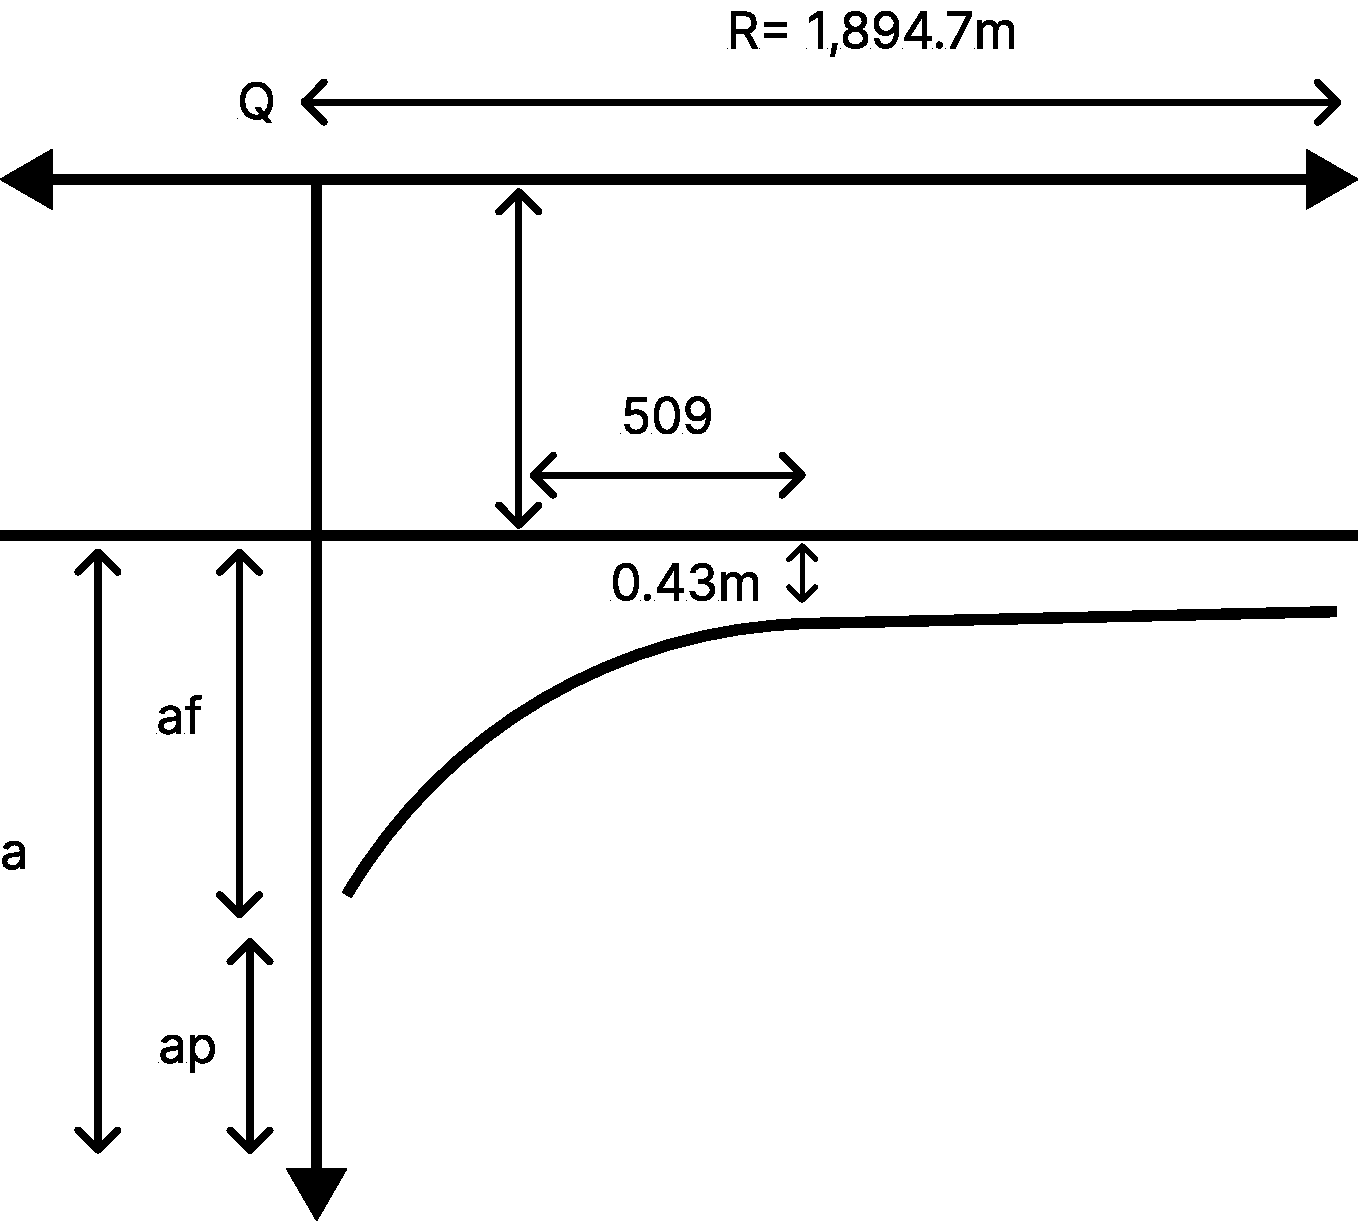
\includegraphics[width=0.5\textwidth]{gh35.pdf}
  \caption{Abatimiento}
  \label{gh35}
\end{figure}
\begin{align*}
    &a_f = \frac{Q}{4\pi T} = \ln{Q} + \frac{2.25Tt}{Sr^2}\\
    &a_f = \frac{0.037}{4\pi (0.018)} \ln{\frac{2.25(0.018)(59,390)}{6.7 \times 10^{ - 4}(0.2032)^2}} = 2.99m\\
    &\eta = \frac{BQ}{a_t} = 0.485\implies a_t = \frac{2.99}{0.485} = 6.165m
\end{align*}
Finalmente el $Q_e$:
\begin{equation*}
    Q_e = \frac{Q}{a_t} = \frac{37 lps}{6.165m} = 6\frac{lps}{m}
\end{equation*}
\end{example}

\subsection{Régimen transitorio en acuíferos semiconfinados}
Probablemente el acuífero más común en la naturaleza es el acuífero semiconfinado. Se ha encontrado que tales acuíferos están cubiertos por estratos poco permeables pero con capacidad suficiente para transmitir cierta cantidad de agua, estos estratos llamados acuitardos, a través de grandes superficies de contacto contribuyen significativamente a la alimentación de los acuíferos. A su vez, los acuitardos pueden estar recargados por zonas saturadas, las cuales pueden estar confinadas o semiconfinadas. La percolacion del agua hacia el acuífero, a través del estrato semiconfinante, se llama filtración por goteo o rezume.

El efecto que introduce el rezume sobre la ecuación en régimen transitorio para acuíferos semiconfinados, puede expresarse matemáticamente. El plano x-y coincide con un estrato completamente impermeable que se toma como plano de referencia para los niveles. Antes que se inicie la extracción de agua, el nivel $h$ del acuífero principal era es constante e igual a la altura H del nivel freático del terreno saturado, o acuífero recargante, medidas ambas sobre el plano de referencia. Una vez iniciado el bombeo, $h$ desciende tal como se presenta en la figura, y puesto que el agua del terreno saturado se mantiene a nivel H, se origina un gradiente hidráulico entre el techo y la base del acuitardo que provocará la aparición del rezume de éste al acuífero principal a través de dicha capa:

La hipótesis que validan las ecuaciones para este tipo de acuiferos en regimen transitorio son las mismas mencionadas para los auciferos ocnfinados. Además, se considera que la conductividad hidráulica K del acuífero principal es lo suficientemente grande comparada con la $k^{\prime}$ del acuitardo como para admitir que el agua se filtre verticalmente y que al llegar al acuífero se refracta con un ánguylo de $90^{\circ}$ prosiguiendo horizontalmente por él. EL abatimiento a (H-h) del nivel piezométrico a una distancia r del pozo de bombeo satisface la ecuación:
\begin{equation}
    B = \sqrt{\frac{T}{\frac{K^{\prime}}{b^{\prime}} }}
\end{equation}
\begin{notation}
    Si B tiende a 0, mayor flujo \begin{itemize}
        \item $b^{\prime}$ valor grande, flujo vertical muy lento, B pequeña
        \item $b$= valor pequeño , B grande
        \item $b^{\prime}\to 0$, se vuelve acuífero libre
    \end{itemize}
\end{notation}
\subsubsection{Método de Hantush (Madhi, 1956)}
Dado que la alimentación por rezume puede llegar a representar un porcentaje significativo del total de agua bombeada por medio de pozos profundos, debemos conocer los métodos para determinar k', T y S.

Hantush y Jacob han propuesto a partir de la solución de la ecuación establecida anteriormente, una curva tupo para el estudio de los abatimiento en régimen transitorio. Las hipótesis para este caso son: Rezume constante, nivel del acuífero recargante constante y refracción horizontal, además de las establecidas para el acuífero confinado, la solución de la ecuación:
\begin{align}
    &a= \frac{Q}{4\pi T} \int_{u}^{\infty} \frac{e^{ - u -\frac{r^2}{4B^2 u}}}{u}\, du = \frac{Q}{4\pi T} W(u,r/B)\\
    &W\left(u,\frac{r}{B}\right) = \int_{u}{\infty} \frac{e^{ - u -\frac{r^2}{4B^2 u}}}{u}\, du\\
    &u = \frac{Sr^2}{4Tt}
\end{align}
Hantush, para las medidas realizadas en un pozo de observación, sugirió el método siguiente (el cual es similar al de Theis):
\begin{enumerate}
    \item Se grafica la función de pozo para este tupo de acuíferos en papel doble logarítmico (1/u), W(u,r/B) y los datos medidos de tiempo, abatimiento (t,a) también en papel doble logarítmico del mismo módulo
    \item Se superponen ambos gráfico manteniendo el paralelismo de los ejes de forma que se ajuste la curva de campo a una de las curvas tupo (r/B) de Hantush
    \item Se elige un punto de ajuste arbitratio (de preferencia de coordenadas cerradas en uno de los dos gráfico), obteniéndose las coordenadas de este, $t_p, a_p$ en la curva de campo y $(a/u)_p, W(u, r/B)$ en la función de pozo. Dichas coordenadas del punto y el valor de $(r/B)_0$ se sustituyen en las fórmulas siguientes
\end{enumerate}
\begin{align}
    T= \frac{Q}{4\pi a_p} W\left(u, \frac{r}{B}\right)_p&& S = \frac{4Tt +p}{\left(\frac{1}{u}\right)_p r^2} && \left(\frac{r}{B}\right)_0 = \frac{r}{\sqrt{\frac{T}{\frac{k^{\prime}}{b^{\prime}}}}}
\end{align}

\begin{example}
    Una unidad acuífera de $10km^2$ está constituida por los siguientes materiales a partir de la superficie:
    \begin{enumerate}
        \item Un acuífero de 10m de espesor de gravas conectado hidráulicamente a un río
        \item Un acuitardo de limos de 12m de espesor ($b^{\prime}$)
        \item Un acuífero de arenas de 50m de espesor ($b$)
        \item El basamento prácticamente impermeable lo forman materiales arcillosos de gran espesor
    \end{enumerate}
EL nivel inicial del acuífero inferior y superior es de 5 metros por debajo de la superficie del suelo. Se construye un pozo de más de 72 metros de profundidad que llega hasta el basamento arcilloso. Dicho pozo de 300mm de diámetro se cementa en la parte superior, dejándose rejilla solamente en el acuífero inferior.

Se afectúa una prueba de bombeo en régimen variable, a un caudal constante de 45 lps, midiéndose los descensos, tanto en el pozo de bombeo como en uno de observación, con las mismas carcterísticas, a 60 metros del de bombeo.

Los resultados son los siguientes:
\begin{table}[h!]
    \centering
    \begin{tabular}{@{}ccc@{}}
    \toprule
    t (min) & \begin{tabular}[c]{@{}c@{}}a(m)\\ P.B.\end{tabular} & \begin{tabular}[c]{@{}c@{}}a(m)\\ P.O.\end{tabular} \\ \midrule
    1    & 0.9  & 0.00 \\
    2    & 1.5  & 0.00 \\
    5    & 2.6  & 0.46 \\
    8    & 3.2  & 0.70 \\
    12   & 3.8  & 1.20 \\
    20   & 4.7  & 1.7  \\
    30   & 5.3  & 2.2  \\
    40   & 5.7  & 2.5  \\
    60   & 6.5  & 3.00 \\
    80   & 7.0  & 3.30 \\
    100  & 7.3  & 3.60 \\
    150  & 8.0  & 4.00 \\
    200  & 8.3  & 4.3  \\
    300  & 9.0  & 4.6  \\
    400  & 9.3  & 4.7  \\
    650  & 10   & 4.9  \\
    800  & 10.3 & 4.95 \\
    1200 & 11   & 5    \\
    1600 & 11.2 & 5    \\
    2000 & 11.3 & 5    \\ \bottomrule
    \end{tabular}
    \caption{Resultados}
    \label{tabgh13}
    \end{table}
\end{example}
% Pozo de bombeo:
% Coordenadas de puntos: $T_p= 100 min= 6000s$, $1/u= 110$, $a_p=7.3m$ y finalmente $W(u,r/B)= 4.1$

\subsubsection{Penetración parcial}
Cuando un pozo capta sólo una parte del espesor saturado del acuífero, se le denomina pozo parcialmente penetrante ($L_c<b$)

En los pozos de penetración parcial los abatimientos son mayores que los provocados en uno totlamente penetrante, para un mismo caudal de extracción, aumentando el abatimiento conforme disminuye la penetración pozo.

Para dar una idea aproximada de la disminución de la eficiencia hidráulica del pozo causado por la penetración parcial, considérese que, si un pozo capta sólo la mitad del espesor saturado de un acuífero, el aatimiento provocado en él, será algo menos que el doble del provocado en un pozo totalemnte penetrante, para le mismo caudal bombeado.

En las proximidades de estos pozos el flujo es tridimensional, por lelo; el abatimiento registrado en el pozo de bombeo y en pozos próximos a él, depende entre otros factores, de la longitud y posición de los cedazos. esto complica la interpretación de las pruebas de bombeo, ya que los abatimientos Son función también de las características constructivas de los posos. Para simplificar la interpretación, es conveniente ubicar los pozos de observación a distancias equivalentes al espesor del acuífero, o mayores, para las cuales el efecto de penetración es mínimo o nulo.

El nivel del agua en un pozo de observación situado a tales distancias se comporta como si el pozo de bombeo fuera totalmente penetrante y la prueba se interpreta en la forma ya indicada.

Cuando se capta la mitad del espesor, el abatimiento en el cono llega a ser casi del doble.

Las Pérdidas de carga en este caso son debidas a la trayectoria de las Partículas . Así , la transmisiviolaol va a estar más alejada de la realidad por estas y las pérdidas de carga por construcción del pozo.

Se recomienda en una penetración parcial que el POZO de observación esté a una distancia mínima de ``b''

Esto es para que la interpretación y obtención de s y t, sea más precisa, pues a partir de esa distancia los efectos de abatimiento extra ya no son considerables. Se recomienda captar la totalidad del acuífero; o mínimo el 70\%.
\subsubsection{Influencia de las características hidráulicas en la forma y extensión del cono de abatimiento}
Se puede analizar la influencia de las características hidráulicas del acuífero en la forma y extensión del cono de abatimientos mediante la expresión simplificada de Jacob para acuíferos confinados en pozos totalmente penetrantes con gasto constantes y en régimen transitorio.

Para esto se tomará un pozo en un acuífero dado, por ejemplo, el siguiente:
\begin{example}
    \begin{enumerate}
        \item Pozo de 18 pulgadas de diámetro (45.72 cm), gasto 50 lps.
        \item Acuífero confinado de transmisividad $1.44\times 10^{-2}\, m^2/s$ y coeficiente de almacenamiento de $1.15\times 10^{-4}$.
        \item Tiempo de bombeo de 3 días.
    \end{enumerate}
\end{example}
Para el mismo gasto . si la permeabilidad se incrementa, profundizan los conos menos.

A mayor S , menor profundidad del Cono y menor radio de influencia.

\subsubsection{Interferencia entre conos de abatimiento}
Admitiendo las hipótesis hechas para la deducción de las ecuaciones de flujo a pozos totalmente penetrantes. Considerando un campo de bombeo en el que existen “n” pozos bombeando cada uno a un gasto constante Qi, el descenso en un punto es la suma de los descensos provocados individualmente por cada uno de los pozos (T y S ctes.).

\begin{equation}
    a_{x,y}= \sum_{i = 1}^{n} Q_iZ\left(r_i,t_i\right)
\end{equation}
\begin{notation}
    para una misma T y S \begin{itemize}
        \item $Q_i$ es el gasto bombeado por el pozo i (si es un pozo de recarga, basta con considerar el gasto negativo). Q negativo son de salida, Q positiva son de entrada 
        \item $r_1$ y $t_1$ son respectivamente la distancia del sitio de coordenadas $x,y$ al pozo ``i'' de coordenadas ($x_i,y_i$), y el tiempo que hace que comenzó el bombeo en dicho pozo
        \begin{equation}
            r_1= \sqrt{\left(x - x_i\right)^2 + \left(y - y_i\right)^2}
        \end{equation}
        \item $Z$ es la función de descenso, que en el caso de régimen permanente, será función de r y en régimen transitorio será función de r y t.
    \end{itemize}
\end{notation}
\begin{align*}
    &Z\left(r_i, t_i\right) = \frac{1}{4 \pi T} \cdot W(u_i)\\
    &a(x,y)= \frac{1}{4\pi T} \sum_{i = 1}^n Q_iW(u_i)
\end{align*}
Para tiempos mayores de $t=2.5Sr^2 /T$, para los que se considera válida la simplificación de Jacob:
\begin{align*}
    &a(x,y)= \frac{1}{4\pi T} \sum_{i = 1}^n Q_i \cdot \ln{\left(\frac{2.25Tt_i}{Sr_i^2}\right)}\\
    &a(x,y)= \frac{1}{4\pi T} \sum_{i = 1}^n Q_i \cdot  \ln{\left(\frac{2.25Tt_i}{S\left[\left(x - x_i\right)^2 + \left(y - y_i\right)^2\right]}\right)}
\end{align*}
Si el acuífero es semiconfinado 
\begin{equation}
    a(x,y)= \frac{1}{4\pi T} \sum_{i = 1}^n Q_i W\left(U_i, \frac{r}{B}\right)
\end{equation}
\begin{problem}[Determinar el tiempo en el que se alcanzan dos conos de abatimiento de dos pozos separados $500m$, en: a) un acuífero libre de $S= 0.1$ y $T= 0.015 m^2/s$, iniciando su operación al mismo tiempo, b) en un acuífero confinado de $S= 1x10^{-4}$ y la misma transmisividad.]
    \textit{ Sol. }
    \begin{align*}
        &R_1+ R_2= N = 500 = \frac{3}{2} \sqrt{\frac{Tt}{S}} + \frac{3}{2} \sqrt{\frac{Tt}{S}} = 3 \sqrt{\frac{Tt}{S}}\\
        &t = \frac{\left(\frac{N}{3}\right)^2S}{T} = \frac{N^2S}{9T} = \frac{500^2 \cdot 0.1}{9 \cdot 0.015} = 185185.2\,s = 3086\,min\\
        & t = \frac{\left(\frac{N}{3}\right)^2S}{T} = \frac{500^2 \cdot 1 \times 10^{ -4}}{9 \cdot 0.015} = 185.185\,s = 3.086\,min\\
    \end{align*}
\end{problem}
\section{Cuantificación de la disponibilidad del agua subterránea}
\subsection{Introducción}
En cada zona, según las condiciones geológicas, climatológicas y topográficas existentes, un cierto volumen de agua de lluvia, que no es medible en forma directa, se infiltra para almacenar a los acuíferos. El volumen infiltrado constituye el recurso renovable del acuífero; su conocimiento es indispensable para planear el aprovechamiento racional de las aguas subterráneas, pues la extracción de un volumen mayor a la recarga media anual induce efectos perjudiciales que en algunas ocasiones, puede llegar a inutilizar el acuífero

Como Objetivo: Determinar la disponibilidad (reserva almacenada y recarga media anual ) de un acuífero.

Se ha intentado cuantificar los volúmenes infiltrados por métodos indirectos, tales como el análisis del ciclo hidrológico y la aplicación de coeficientes de infiltración.
\subsubsection{Balance hidrológico superficial}
La estimación del escurrimiento, precipitación evaporación, nos permite calcular la infiltración por diferencia en la ecuación del ciclo hidrológico
\begin{equation}
    I= P-E-S
\end{equation}
El escurrimiento superficial puede conocerse en forma más o menos aproximada, mediante estaciones hidrométricas instaladas en las corrientes que drenan el área.\footnote{Recarga: Lo que llega a la zona saturada. Este método no nos permite calcular la reserva almacenada.}
\subsubsection{Método de coeficientes de infiltración}
Éste método consiste en aplicar coeficientes de infiltración a las formaciones geológicas que afloran en el área estudiada. Éstos coeficientes hipotéticos representan el volumen infiltrado en una cierta formación, expresada por un porcentaje del volumen medio de lluvia precipitada sobre la misma.

Consiste en asignarle a una cierta área parcial de un área total en la que estamos queriendo determinar la potencialidad de un acuífero. A esa pequeña área (Ai) se le va a asignar un coeficiente de infiltración (Ci) dependiendo de la formación geológica que aflore en la superficie; se van a superponer isoyetas y se ponderarán.
\begin{equation}
    V_i= \sum_{i=1}^n C_iP_i A_i
\end{equation}
Limitante: el $C_i$ representa un porcentaje que va atravesar la superficie del suelo, un porcentaje de la precipitación. Esa infiltración guarda relación con la naturaleza del material que aflora, la intensidad de la lluvia, contenido de humedad inicial, topografía, cubierta vegetal. Además, este método no determina ni recarga ni reserva almacenada.

Los métodos indirectos son totalmente inadecuados para determinar la potencialidad de un acuífero; ya que, los valores obtenidos por estos métodos carecen de validez debido al gran número de variables que afectan.
\subsubsection{Balance de agua subterránea}
La forma más adecuada de cuantificar la potencialidad de los acuíferos, utilizan un método que trabaje directamente con el espesor saturado, considerando el agua ya infiltrada y relativamente al margen de los fenómenos que ocurren en la superficie, dicho método recibe el nombre de balance de agua subterránea.

Se basa en el principio de conservación de la materia en un intervalo de tiempo dado.

Determina la recarga vertical anual y reserva almacenada

\begin{itemize}
    \item Recarga \begin{itemize}
        \item Flujo subterráneo ($E_h$)
        \item Recarga vertical ($R_v$)
        \item Corriente superficial (D)
    \end{itemize}
    \item Descarga \begin{itemize}
        \item Flujo subterráneo ($S_h$)
        \item Corriente superficial (D)
        \item Obras de captación de aguas subterránea ($B$)
        \item Evapotranspiración en niveles freáticos someros ($E_v$)
    \end{itemize}
\end{itemize}
\begin{equation}
    E_h + R_v - S_h - B - E_{vt} \pm D = \pm \Delta V= \Delta V^{\prime}S
\end{equation}
Esta expresión es la ecuación general de balance de aguas subterráneas

Información necesaria para el balance
\begin{enumerate}
    \item Área de balance
    \item Periodos de análisis
    \item Recolección y análisis de niveles de agua \begin{enumerate}
        \item Toma de datos de niveles
        \item Organización de la información
        \item Procesamiento e interpretación de la información \begin{enumerate}
            \item Configuración de profundidad de nivel estático (PNE)
            \item Configuración de elevación del nivel estático (ENE)
            \item Configuración de evolución del nivel estático (EvNE)
            \item Hidrógrafos de pozos
        \end{enumerate}
    \end{enumerate}
    \item Plano de isotransmisividad
    \item Perfiles hidrogeológicos
    \item Hidrometría de aprovechamientos Q,t, volumen extraído
\end{enumerate}
\subsubsection{Área de balance}
El área utilizada para efectuar el balance de agua subterránea depende de varios factores. Por una parte, lo ideal sería efectuar el balance para todo el acuífero (valle, planicie) a fin de conocer su potencialidad, sin embargo, esto no siempre es posible, debido a que la aplicación del balance requiere del conocimiento del comportamiento del acuífero observado en pozos los cuales no siempre se encuentran distribuidos en toda el área, sino solo en una porción de la misma. Por consiguiente, en muchas ocasiones el área de balance tiene que limitarse al área con datos disponibles

Otras veces aun cuando se dispone de información acerca del comportamiento y características de todo el acuífero, pueden interesar, por alguna razón, conocer el funcionamiento y potencial de una porción del mismo. En este caso el área se balance se limitará a esa porción. El área de balance puede estar limitada por fronteras reales (geológicas e hidrológicas tales como rocas impermeables o cuerpos de agua) y/o virtuales (límites políticos territoriales, áreas de interés, disponibilidad de información)


\subsubsection{Periodos de análisis}
Siempre se plantea una ecuación de balance, es necesario tener una idea más o menos clara del comportamiento del acuífero a estudiar La cuantificación del potencial de un acuífero se basa en la evolución de los niveles del agua subterránea por bombeo en pozos y de la determinación de la res de flujo subterráneo. El fenómeno de la recarga de un acuífero se presenta en forma cíclica por lo que para su cuantificación es necesario obtener información por lo menos durante un año, determinándose con esto, un valor preliminar; sin embargo, la recarga no es constante en el tiempo, sino que varía de un año a otro, dependiendo de las condiciones naturales y artificiales que influyen en el comportamiento de los acuíferos por lo que para obtener un valor medio de recarga anual es necesario considerar varios años. Dependiendo de la información disponible se pueden plantear un determinado número de ecuaciones de periodos incluso no constantes.
\begin{table}[h!]
    \centering
    \begin{tabular}{@{}ccc@{}}
    \toprule
    Ecuación no.                                  & Periodo           & años  \\ \midrule
    $Eh_1+Rv-Sh_1-B_1-E_{vt1}\pm D_1=\Delta V_1S$ & Oct/2002-Jun/2004 & 1.667 \\
    $Eh_2+Rv-Sh_2-B_1-E_{vt2}\pm D_2=\Delta V_2S$ & Jun/2004-Jun/2005 & 1.0   \\
    $Eh_3+Rv-Sh_3-B_3-E_{vt3}\pm D_3=\Delta V_3S$ & Jun/2005-jul/2007 & 2.083 \\
    $Eh_4+Rv-Sh_4-B_4-E_{vt4}\pm D_4=\Delta V_4S$ & Jul/2007-Oct/2009 & 2.25 \\ \bottomrule
    \end{tabular}
    \caption{Ejemplo de sistema de ecuaciones con sus periodos respectivos según información disponible y consistente.}
    \label{tabgh14}
\end{table}
\subsubsection{Recolección y análisis de niveles de agua}
\textbf{Toma de datos de niveles de agua}:
Se requiere responder 3 preguntas para programar un sistema de observaciones de niveles ¿Cómo? ¿Cuándo? ¿Donde deben realizarse las mediciones correspondientes? Respecto al ¿cómo? Es posiblemente la pregunta más fácil de responder, ya que se realizan con sondas eléctricas, que consisten fundamentalmente de un cable de dos

De dos hilos, unidos por un extremo a una pila y por el otro con los dos hijitos ligeramente separados, los que al contacto del agua permite el paso de la corriente eléctrica que se registra con un miliamperímetro. El cable se introduce por un hueco que puede haber en el cabezal de descarga de la BTV o un orificio hecho a propósito, y se desliza entre la tubería de ademe y la columna de la bomba, la longitud de cable que logra introducirse hasta que se logra el contacto de la sonda con el agua, puede medirse y determinar la posición del nivel del agua con respecto a un punto de referencia, el que se debe elegir previamente y mantenerse para futuras mediciones.

Si se pretende definir el ¿cuándo se recomiendan efectuar las observaciones? Existen dos respuestas. La primera corresponde a pruebas en condiciones dinámicas, conocidas como pruebas de bombeo y cuya secuencia de observación se definió en Hidráulica de pozos

Cuando las mediciones se efectúan con el interés de definir el comportamiento del acuífero a nivel regional, sometido a diferentes condiciones de recarga y descarga, es importante fijar un programa que permita cumplir con el objetivo perseguido, requiriéndose entender de antemano cuál es la pretensión del trabajo a realizar.

Práctica común en estos casos puede ser la toma inicial de niveles con una frecuencia mensual por un periodo mínimo de un año, de tal forma que durante ese tiempo se tengan datos correspondientes a las diferentes situaciones bajo las cuales se encuentra el acuífero, por ejemplo: periodo de lluvia, régimen variable de bombeo, escurrimientos superficiales, riego de superficies agrícolas.

De las condiciones anteriores, resulta que en el caso más frecuente de estudio de una región agrícola, abastecida con agua subterránea, las observaciones pueden ser dos o tres por año, al inicio y terminación del periodo de riego que puede corresponder también al inicio y terminación de la temporada de lluvias, lográndose en esa forma detectar los máximos cambios que se presentan por los efectos más notables que los producen. En los distritos de riego del noreste del país las observaciones del nivel estático se realizan anualmente en el mes de octubre.

¿Dónde es conveniente programar observaciones? Se requiere contar con datos suficientes que permitan conocer los aspectos fundamentales de un acuífero, en este sentido se debe destacar la necesidad de tener una idea sobre las condiciones geohidrológicas, para decidir sobre los pozos piloto.

Un pozo piloto debe de tener información lo más completa y consistente posible, que represente la carga fidedignamente de una cierta porción del mismo acuífero a cuantificar.

Como ejemplo puede señalarse la existencia de una zona de varios acuíferos, cuyo nivel piezométrico es diferente, debiéndose conocer tal situación, para efectuar un procesamiento adecuado, y decidir sobre los puntos de observación. En otras ocasiones, de las mediciones de niveles de agua resultan deficiencias notables en áreas muy próximas, que sugieren la necesidad de una investigación que permita encontrar la causa de tal deficiencia y tomarla en cuenta en el procesamiento.


\textbf{Organización de la información:}

Con la recomendación complementaria anterior, resulta conveniente destacar la forma para organizar la información piexométrica obtenida en una zona. En primer lugar, contando ya con los puntos de observación seleccionados, es conveniente que los recorridos sistemáticos se realicen en el menor tiempo posible, de tal forma que la información que se obtenga corresponda a una misma condición de operación del sistema acuífero. En segundo término, al hablar de un sistema de mediciones, este debe ser establecido procurando que año con año se cuente con datos correspondientes a condiciones semejantes, de la forma que sea posible establecer comparaciones de las mediciones obtenidas a través del tiempo.

Una manera de guardar la información sería establecer un archivo de datos piezométricos, diferenciando en cada ocasión si la medida corresponde a condicines dinámicas o estáticas en el pozo. Posteriormente, las medidas subsecuentes deben clasificarse y agruparse por punto de observación, indicando siempre la fecha correspondiente al dato medido.

Bases de datos de todos los pozos (incluyendo pozos piloto)

Las formas más comunes que se utilizan para procesar y determinar características geohidrológicas de un acuífero, consisten en la elaboración de planos conteniendo curvas de igual elevación o evolución piezométrica, o bien, planos de profundidades al nivel del agua.

También se construyen hidrógrafos regionales o de pozos y perfiles destacando los niveles piezométrios.

Configuración de profundidad de los niveles estáticos (PNE):

La elaboración de planos conteniendo curvas de profundidad al nivel estático, es semejante a la comentada, condición que implica tener los conocimeitnso básicos regionales y efectuar una depuración previa de los datos medidos, de tal forma que se elabore una configuración confiable que consdiere todos los efectos que puedan influir en su forma.

Respecto a la utilidad de estas curvas se debe señalar que define zonas donde los niveles se encuentran más cercanos a la superficie del terreno, identificándose por consiguiente, áreas de descarga por evapotranspiración o en caso de superficies de riego, zonas de drenaje problemático.

Configuraciones de elevación del nivel estático:

Las configuraciones de elevaciones del nivel estático representan la forma de la superfiice piezométrica de un acuífero confinado o semiconfinado, y la forma de la superficie freática en acuíferos libres.

Las configuraciones se preparan con base en los niveles estáticos referidos a un plano horizontal, generalmente el nivel medio del mar. El procesamiento consiste en trazar curvas de igual elevación del nivel estático, interpolando entre valores conocidos.

En primer lugar, es necesaria una depuración de los datos, ya que pueden estar afectados, por ejemplo: Un nivel de agua detectado puede estar influenciado por el bombeo de algún pozo vecino, y por lo tanto no ser representativo del nivel estático, un falso contacto de la sonda o una medición equivocada de la longitud del cable introducido para lograr el contacto, lleva a un estático completamente falso.

Las configuraciones así obtenidas proporcionan información respecto a las direcciones de flujo, localización de zonas de recarga, gradientes hidráulicos, comportamiento de las fronteras, efectos de la explotación, otros.

Por otra parte las configuraciones de las elevaciones del nivel estático del agua subterránea son indispensables para la cuantificación de caudales de flujo subterráneo. Esta cuantificación se basa en el concepto de red de flujo y en la Ley de Darcy. Debe entenderse que las curvas de igual elevación del nivel estático corresponden a líneas equipotenciales, por lo que el flujo subterráneo debe ocurrir sobre líneas normales a éstas denominándole entonces a las líneas perpendiculares, líneas de flujo. A la malla formada por las líneas equipotenciales y líneas de flujo se le llama red de flujo.

La elevación del nivel estático (ENE) en un pozo, para un mes/año, se obtiene restando a la elevación del brocal de dicho pozo, la PNE de la misma fecha.

Con base en la expresión de coeficiente de permeabilidad de Darcy, puede cuantificarse el caudal de flujo que circula a través de una sección (canal de flujo o celda de flujo), limitada por dos líneas de flujo y dos curvas equipotenciales en la forma siguiente:
\begin{equation}
    Q =Av = Bb \cdot Ki= BTi = BT \frac{\Delta h}{L}
\end{equation}

Configuración de evoluciones del nivel estático:

La elaboración de planos conteniendo curvas de igual evolución del nivel estáticos que se obtiene de la observación sistemática de la posición de los niveles estáticos, cuya comparación y de acuerdo con la diferencia obtenida en un intervalo de tiempo considerado, constituye el elemento básico para elaborar la configuración correspondiente.

La importancia de las curvas de igual evolución reside en que manifiestan los cambios registrados en el almacenamiento de un acuífero, en un periodo y bajo ciertas condiciones, pues define áreas de abatimiento o descensos de los niveles estáticos, es decir, áreas donde ha disminuido o aumentado el volumen de agua almacenando.

Esta información relacionada con el bombeo de pozos, ilustra los efectos que ha tenido la explotación en el acuífero.

La evolución del nivel estático en un pozo para un periodo (ej. Junio/2010-Jul/2012) se determina restando su elevación del nivel estático final del periodo, a la elevación del nivel estático inicial del mismo periodo, dicha evolución podrá ser negativa (en el caso de abatimiento de niveles estáticos) o positiva (en el caso de recuperación de niveles estáticos).
\begin{align*}
    EvNE(\text{Jun/2010-Jul/2012}) = ENE_{(\text{Jul/2012})}- ENE_{(\text{Jun/2010})}\\
    EvNE(\text{Jun/2010-Jul/2012}) = PNE_{(\text{Jun/2010})}- PNE_{(\text{Jul/2012})}
\end{align*}

Hidrógrafos de pozo:

Una de las prácticas más comunes consiste en comparar observaciones en un mismo punto y en caso de resultar algún dato anormal a juicio del procesador, se elimina, requiriéndose experiencia para efectuar tal decisión en forma acertada. Entre las formas que facilitan tal actividad, conviene destacar la construcción de hidrógrados de pozos, que consisten en un sistema de coordenadas, en el cual en las abscisas se maneja el tiempo y en las ordenadas la profundidad o la elevación del nivel estático. Con tal gráfica un dato fuera de la tendencia, inmediatamente se identifica, recomendándose por consiguiente una revisión antes de eliminarlo.

Una ventaja más que hace recomendable la elaboración de los hidrógrafos, está en la facilidad que presentan para conocer en un mismo punto los cambios de niveles que ocurren con el tiempo, fluctuaciones cuyo análisis son importantes de conocer en la realización de un estudio geohidrológico, pues permiten identificar con conocimientos adicionales, los efectos predominantes que modifican las condiciones geohidrológicas regionales.

\subsubsection{Plano de isotrasmisividad} 
Para la cuantificación del flujo subterránea de salidas y entradas a un acuífero, es importante la realización de pruebas de bombeo, principalmente en la frontera donde ocurre ficho flujo, con el objeto de conocer los parámetros hidráulicos del acuífero regionalmente. Para la modelación de acuíferos es imprescindible contar con las permeabilidades y transmisividades en todo el acuífero, con el objeto de simular su funcionamiento y hacer predicciones.

\subsubsection{Perfiles hidrogeológicos}
Una práctica común en la interpretación de la información geohidrológica, es la elaboración de perfiles definiendo las formaciones geológicas del subsuelo y señalando a la posición de los niveles del agua.

Este tipo de trabajos en ocasiones es muy ilustrativo, nos permite dar objetividad a la presentación de resultados a estimar espesores y volúmenes almacenados de agua.
\subsubsection{Hidrometría de los aprovechamientos}
Este concepto se refiere a los diferentes métodos que se siguen para cuantificar los volúmenes de descarga tanto natural como artificial, de las aguas subterráneas. De hecho el volumen de descarga de agua subterránea más significativo, lo constituye las extracciones mediante pozos de bombeo, dependiendo estas, de la zona explotada y el uso a que se destine el agua. La determinación de dicho volumen se hace en base a un censo de pozos, seleccionándose de él, los aprovechamientos que por características de su equipo de bombeo y/o su régimen de operación, tenga una influencia significativa en el volumen total.

Según el uso o usos a que se destine el agua de los pozos seleccionados, se eligirá la forma más conveniente de estimar sus volúmenes de extracción (en ausencia o para confirmar lo reportado por el medidor volumétrico que debe estar instalado en la descarga). Entre los métodos que pueden utilizarse se tienen:
\begin{enumerate}
    \item Medidor totalizador de flujo
    \item Consumo de energía eléctrica (recibo de CFE), potencia consumida y caudal
    \item Tiempo de operación y caudal
    \item Superficie y lámina de riego
    \item Técnicas de muestreo, con diámetros de descarga, uso y volumen de extracción
    \item Volumen de extracción de cada pozo del Registro Público de Derechos de Agua (REPDA)
\end{enumerate}
Generalmente el volumen de extracción de todos los aprovechamientos, cuya extracción individual es poco significativa (pozo no equipado o pozo equipado con bomba de diámetro menor a 2") se estima en forma global.

Un dato importante en la hidrometría de los aprovechamientos que cuentan con equipo de bombeo, es la determinación del caudal que descargan, el cual se puede conocer mediante el aforo de los pozos. Los métodos más utilizados en el campo son el del orificio calibrado y la escuadra.

\subsection{Cuantificación de los términos de la ecuación de balance de aguas subterráneas}

Para hacer la cuantificación de los términos que constituyen la ecuación de balance es necesario contar de antemano con información de obtenida en el campo, tal como la localización de los pozos, los cuales deberán ubicarse en un plano con le fin de conocer su distribución, que es la que generalmente delimita el área en que se efectuará el balance; las lecturas de los niveles estáticos obtenidas periódicamente en los pozos piloto, la hidrometría de todos los aprovechamientos subterráneos existentes dentro del área de balance, las características hidráulicas del acuífero obtenidas con las pruebas de bombeo y los datos geológico geofísicos mediante los cuales se determinan las fronteras laterales e inferiores del acuífero que se encuentra del área de estudio.

\subsubsection{Entradas y salidas por flujo subterráneo (Eh y Sh)}
Los volúmenes de entradas y salidas por flujo subterráneo, se obtienen multiplicando los caudales de flujo que pasan por el perímetro del área de balance, calculados como se indicó anteriormente, por el intervalo de tiempo para plantear el balance. La expresión matemática para calcular entradas es:

En una configuración de ENE, se crea la red de flujo y se suman los gastos de todas las celdas de flujo de entrada ($Q_{Eh}$) y las de salidas ($Q_{Sh}$)
\begin{equation}
    Q_{Eh}= \sum_{j = 1}^{nc}T_jB_j\frac{\Delta h_j}{L_j}
\end{equation}
Para Oct/2002-jun/2004: 
\begin{equation*}
    E_{h1} = \frac{Q_{oct}\text{/2002} +Q_{jun}text{/2004}}{2} \times t_{oct\text{/2002} - jun\text{/2004}} 
\end{equation*}
En la que $T_j$ es la transmisividad de la celda de flujo ``j'', $B_j$ ancho medio de canal de flujo ``j'', $\Delta h_j$ diferencia entre valores de equipotenciales de la celda de flujo ``j'', $L_j$ es la longitud media de la celda de flujo ``j'', y t es el intervalo de tiempo para plantear el balance. ``nc'' es el número de canales de entrada definidos en la periferia del área de balance. Los valores de B y L se miden directamente en la red de flujo.
\begin{example}
    $C_r: \, B=3.7km\, L=324m\, T=0.012m2/s,\,\Delta h=2m$
    \textit{ Sol. }

    \begin{align*}
        Q_4 =\left(3700\right) \cdot \left(0.032\right) \cdot \left(\frac{3}{324}\right)= 0.274 \frac{m^3}{s}\\
        Q_{oct /2002} = 3.721 \frac{m^3}{s}\land\quad Q_{jun / 2004}= 3.38 \frac{m^3}{s}\\
        Eh_1 = \frac{3.721 + 3.38}{2} \cdot 1.667 \cdot 60 \cdot 60 \cdot 24 \cdot 365 = 186.61 \times 10^6 m^3
    \end{align*}
\end{example}
\subsubsection{Descarga por medio de manantiales o como flujo base de corriente superficial (D)}
Este término se cuantifica mediante estaciones de aforo, en las cuales se registran ls volúmenes que descarga el acuífero, durante el periodo de tiempo considerado para el balance. Generalmente se aplica el análisis de los hidrogramas en su componente de la curva de recesión o decaimiento.

\subsubsection{Extracción por bombeo}
Podría conocerse fácilmente y con buena precisión, si los pozos contarán con medidores instalados en la descarga de los equipos de bombeo. Como esto no se tiene en la mayoría de los casos, es necesario recurrir a estimaciones indirectas, basadas en superficiales y láminas de riego (en áreas agrícolas) o en caudales y tiempos de bombeo y otros métodos.

\subsubsection{Evapotranspiración}
Como ya se indicó anteriormente, este término sólo tiene significado dentro de la ecuación si en el área de estudio existen áreas con nivel freático somero (en la configuración de profundidades del N.E.), calculándose mediante la aplicación del valor de la evaporación potencial media o por la fórmula empírica del L. Turc. En forma práctica, dependiendo de la posición de los niveles freáticos (0-5 m) se puede aplicar un porcentaje de la evapotranspiración potencial que puede ser entre 70\% y 90\% de ésta.

Se puede estimar a partir de la evaporación potencial, con los valores siguientes:
\begin{table}[h!]
    \centering
    \begin{tabular}{@{}cc@{}}
    \toprule
    PNE (m) & \% de Evap. Pot. \\ \midrule
    0-1     & 80               \\
    1-5     & 60               \\
    5-10    & 40               \\ \bottomrule
    \end{tabular}
    \caption{Evaporación potencial}
    \label{tabgh15}
\end{table}
O con la fórmula de L. Turc para valores de 0-20 de PNE
\begin{equation}
    E_{TR}= \frac{p}{\sqrt{0.9 + \frac{p^2}{L^2}}}
\end{equation}
\begin{notation}
    \begin{itemize}
        \item p: Precipitación media anual mm
        \item $L= 300+25T+ 0.05T^3$
        \item T: Temperatura media anual $^{\circ}C$
        \item Válida para $E_{TR}<pp$
    \end{itemize}
\end{notation}
También se puede estimar con la fórmula de Coutagne
\begin{equation}
    E_{TR} = p + xp^2
\end{equation}
\begin{itemize}
    \item p: Precipitación en m/año
    \item $x= \frac{1}{0.8}x\leq p\leq \frac{1}{2}x$
\end{itemize}
\begin{example}
    Área (con PNE<20m)= $23km^2$, Pp= 1135mm y $T=19.2^{\circ}C$

    \textit{ Sol. }

    Con la fórmula de L. Turc (p en mm):
    \begin{align*}
        &E_{TR}= \frac{p}{\sqrt{0.9 + \frac{p^2}{L^2}}}\\
        &L= 300+25T+ 0.05T^3
    \end{align*}
    Resulta $L=1133.89$ y $E_{TR}= 823mm$

    Con la fórmula de Coutagne, (p en m):
    \begin{align*}
        E_{TR} = p - xp^2\\
        x = \frac{1}{0.8 + 0.14T}
    \end{align*}
    Resulta x= 0.2867, lo cual cumple con la condición $1/(2.293)<p<1/(0.5734),\, 0.436<1.135<1.744$
    \begin{align*}
        &E_{TR}= 765mm\\
        &E_{VT}= E_{VT} = 14.3 \times 10^6 m^3\, jun / 2004\\
        &E_{VT1} = \left(\frac{18.62 + 14.3}{2}\right)  \cdot 1.667 = 27.43 \times 10^6 m^3
    \end{align*}
    
\end{example}
\subsubsection{Volumen drenado o saturado}
se calcula a partir de la Configuración de evolución de los niveles estáticos y del coeficiente de almacenamiento del acuífero. La expresión matemática que se utiliza es la siguiente:
\begin{align}
    &\Delta V^{\prime}_{acuifero}= \pm \sum_{i = 1}^{n} a_i \bar{h}_i\\
    &\Delta V_{agua}= \pm S \sum_{i= 1}^{n} a_i \bar{h}_i
\end{align}
\begin{notation}
    \begin{itemize}
        \item S: Coeficiente de almacenamiento
        \item $a_i$ es un elemento de área con evolución $h_i$ y $n$ es el número de elementos en que se divide el área de balance
    \end{itemize}
\end{notation}
Mediante curvas de igual evolución del nivel estático corresponde al intervalo de tiempo seleccionado para plantear el balance, se calcula, en el caso de un acuífero confinado es la variación total de la presión. En algunos casos, el coeficiente de almacenamiento se determina mediante pruebas de bombeo, o bien se infiere de acuerdo a los materiales que constituyen al acuífero, cuando no existe tal información o su valor regional es dudoso, se introduce en la ecuación de balance como una incógnita más.

\subsubsection{Recarga vertical (Rv)}
Como ya se indicó, no puede obtenerse en forma directa, y sólo puede cuantificarse despejándolo de la ecuación. Para incluirla en la ecuación, o ecuaciones de balance, es necesario por lo menos un conocimiento aproximado de su forma de ocurrencia y su distribución en el tiempo. Es necesario saber, por ejemplo, si la recarga al acuífero se concentra en unos cuantos meses del año, o si ocurre a lo largo de todo el año como en el caso de zonas agrícolas regadas con agua superficial, en la que en los terrenos de riego, las pérdidas por infiltración en los canales no revestidos y los coleos alimentan al acuífero en forma prácticamente continua.

\subsection{Solución de las ecuaciones de balance}
Dado que la recarga es un fenómeno cíclico, se calcula su valor por ciclo, es decir por año. El número de ecuaciones de balance que deben plantearse, dependerá en cada caso, del número de incógnitas a despejar.Si la única incógnita es la recarga, bastará con plantear una ecuación, que pueda ser la correspondiente a un año o la fracción del mismo en la que se ocurra la recarga. La solución de la ecuación proporcionará la recarga anual buscada. (En este caso se requiere del conocimiento del coeficiente de almacenamiento regional). 
Si además de la recarga se tiene otra incógnita (S, coeficiente de almacenamiento regional), será necesario plantear mínimo dos ecuaciones, correspondientes a intervalos de tiempo independientes, que pueden ser dos fracciones complementarias de un año.

En cualquier caso, deberá contarse con la información necesaria para obtener los valores de los términos restantes de la ecuación, correspondientes a los intervalos de tiempo seleccionados; es decir, deberá contarse con las configuraciones de niveles estáticos correspondientes al inicio y final de cada intervalo, y deberá conocerse la evolución de los mismos niveles y el volumen descargado por el acuífero, en cada uno de dichos intervalos.

En general, una evolución basada en la información correspondiente a un año, proporcionará una idea preliminar de la recarga al acuífero y de las condiciones de explotación en que se encuentra el mismo, Sin embargo, como la recarga no es constante en el tiempo, sino que varía de un año a otro con la cuantía y distribución de la precipitación en el tiempo y en el espacio, entre otros factores; es necesario obtener la recarga correspondiente a varios años con diferentes condiciones de precipitación, con el fin de obtener una recarga media anual.

\begin{example}
    Sistema de ecuaciones con sus periodos respectivos según información disponible y consistente (ecuación, periodo y años):
    \begin{align*}
        Eh_1 + R\upsilon - Sh_1 - B_1 - E_{VT1} \pm D_1 = \Delta V_1 S && oct / 2002 - jun / 2004&& 1.667\\
        Eh_2 + R\upsilon - Sh_2 - B_2 - E_{VT1} \pm D_2 = \Delta V_2 S && jun / 2004 - jun / 2005&& 1.000\\
        Eh_3 + R\upsilon - Sh_3 - B_3 - E_{VT1} \pm D_3 = \Delta V_3 S && jun / 2005 - jul / 2007&& 2.083\\
        Eh_4 + R\upsilon - Sh_4 - B_4 - E_{VT1} \pm D_4 = \Delta V_4 S && jun / 2007 - oct / 2009&& 2.417\\
    \end{align*}
\end{example}
\textit{ Sol. }

Se requiere primeramente anualizar las ecuaciones (si el periodo de cada ecuación no es anual), y esto se hace simplemente dividiendo cada uno de los términos de la ecuación, entre el número de años de cada una de ellas. De esta forma la recarga vertical será directamente su valor medio anual en el periodo correspondiente.

Despejando se tiene:
\begin{equation*}
    Eh - Sh - B - E_{VT} + D =\Delta VS- R\upsilon
\end{equation*}
La cual es un model lineal de tipo $y = mx + b$
\begin{align*}
    &Eh - Sh - B- R_{VT} \pm D= y\\
    &\Delta V = x\\
    &S = m\\
    &R\upsilon = b
\end{align*}

\subsubsection{Reserva almacenada}
La reserva almacenada es el volumen de agua que a través de miles de años se ha acumulado en el acuífero. Se determina multiplicando el espesor medio saturado, el área y el coeficiente de almacenamiento del acuífero, el cual se conoce al resolver las ecuaciones de balance:
\begin{equation}
    \text{Reserva almacenada}= A_b \bar{b}S
\end{equation}
\begin{example}
    Sistema de ecuaciones del acuífero de Caborca Sonora, de la tabla:
    \begin{table}[h!]
        \centering
        \begin{tabular}{@{}cccccccccc@{}}
        \toprule
        Periodo & $Eh$ & B   & $\Delta V(x)$ & Eh-B(y) & x    & y   & Déficit & Abat. (m) & $\Delta v/A$ \\ \midrule
        68-69   & 48   & 308 & -770          & -260    & 770  & 260 & 104.55  & 0.56      & 0.55         \\
        69-70   & 53   & 356 & -1152         & -303    & 1152 & 303 & 147.55  & 0.80      & 0.83         \\
        70-71   & 48   & 325 & -913          & -277    & 913  & 277 & 121.55  & 0.66      & 0.66         \\
        71-72   & 45   & 288 & -631          & -243    & 631  & 243 & 87.55   & 0.47      & 0.45         \\
        72-73   & 48   & 285 & -662          & -237    & 662  & 237 & 81.55   & 0.44      & 0.48         \\
        73-74   & 47   & 355 & -1106         & -308    & 1106 & 308 & 152.55  & 0.83      & 0.80         \\
        74-75   & 50   & 327 & -910          & -277    & 910  & 277 & 121.55  & 0.66      & 0.65         \\ \bottomrule
        \end{tabular}
        \caption{Área de balance: $1,360 km^2$ en metros: $1390\times 10^{6}m^2$}
        \label{tabgh16}
    \end{table}
    La suma $\sum \Delta V(x)=-6,144$
    Reserva almacenada a 50m de espesor:
\begin{equation*}
    R = AbS = 1390 \times 10^6 m^2(50m)(0.133) = 
\end{equation*}
Recordando que se trata de un acuífero costero, para 1996 el $\Delta V= -1800\times 10^6m^3$ de volumen drenado.

Del último balance $A=2758km^2$, para 2007 el $\Delta V=-1200\times 10^6m^3$ y abatimiento medio de 0.43m. Con ENE de 450 a -5 MSNM.
\end{example}